\documentclass[12pt, oneside, a4paper]{extreport}
\usepackage{epsfig}
\usepackage{amsmath}
\usepackage{threeparttable}
\usepackage{rotating}
\usepackage{lscape}
\usepackage{supertabular}
\usepackage{amssymb}
\usepackage{afterpage}
\usepackage{fancyhdr}
\usepackage[bf]{caption_pmo}
\usepackage{pifont}
\usepackage{dcolumn}
\usepackage{multirow}
\usepackage{graphicx}
\usepackage{mathrsfs}
\usepackage{hhline}
\usepackage{color}
\usepackage{fancybox}
\usepackage{cite}
\usepackage{float}
\usepackage{here}
\usepackage{enumitem}
\usepackage{ragged2e}
%\usepackage[dvips]{color}
\usepackage{graphics}
\usepackage{theorem}
\usepackage{boxdims}
\usepackage{pstricks}
\usepackage{epsfig}
\usepackage{subfigure}
\usepackage{siunitx}
\usepackage{xcolor,colortbl}
\usepackage{boldline,multirow}
%\usepackage[font=normalsize,labelfont=bf]{caption}
\usepackage[font=normalsize,labelfont=bf]{caption}
\usepackage{times}
\usepackage[nottoc]{tocbibind}
\usepackage{makecell}


\setlength{\parskip}{0.5cm}



\usepackage[up,bf,raggedright]{titlesec}
%\usepackage{blindtext}

\titleformat{\chapter}[display]
 {\normalfont\Large\bfseries\huge}{\filright\chaptertitlename\ \thechapter} {20pt}{\Large\huge\filright}
\titlespacing*{\chapter}{0pt}{-50pt}{20pt}
%\titleformat{\chapter}{\filright\normalfont\huge\bfseries}{\thechapter.}{20pt}{\huge}



%\usepackage{kantlipsum}
%\fancyhf{} % clear all header and footers
%\renewcommand{\headrulewidth}{0pt} % remove the header rule
%\fancyfoot[CE,CO]{\thepage} % Left side on Even pages; Right side on Odd pages
%\pagestyle{fancy}
%\fancypagestyle{plain}{%
%  \fancyhf{}%
 % \renewcommand{\headrulewidth}{0pt}%
 % \fancyhf[lef,rof]{\thepage}%
%}



%\pagestyle{fancy}
%\fancyhf{}
%\cfoot{\thepage}
 %\renewcommand{\headrulewidth}{0pt}%
 % \renewcommand{\footrulewidth}{0pt}%



\usepackage[left=2cm, right=2cm, top=2cm, bottom=4cm]{geometry}

\newcommand{\cy}[1]{\citeyear*{#1}}  % year NO brackets
\newcommand{\sun}{\hbox{$\odot$}}
\newcommand{\degr}{^{\circ}}  % degree symbol
\newcommand{\fdg}{\hbox{$.\!\!^\circ$}}  % . and degree
\newcommand{\textbfit}[1]{\textbf{\textit{#1}}}
\newcommand{\mathbfit}[1]{\textbf{\textit{#1}}}
\newcommand{\textbfss}[1]{\textbf{\textsf{#1}}}
\newcommand{\mathbfss}[1]{\textbf{\textsf{#1}}}
\newcommand{\bmath}[1]{\mathbfit{#1}}   % meant to be bold math symbol
\renewcommand{\captionsize}{\small}

\newlength{\eqntop}    % space to add between text and top of equation
\newlength{\eqnbot}    % space to add between bottom of eqn and text
\setlength{\eqntop}{1mm}  % move equations up
\setlength{\eqnbot}{0mm}     % no change

\setlength{\abovedisplayskip}{0mm}
\setlength{\belowdisplayskip}{10mm}
\setlength{\abovedisplayshortskip}{0mm}
\setlength{\belowdisplayshortskip}{10mm} \setlength\arraycolsep{2pt}

%\setcounter{secnumdepth}{3}
%\setcounter{tocdepth}{3}



\newtheorem{theorem}{Theorem}
\newtheorem{lemma}{Lemma}

\def\tr{\mathop{\rm tr}\nolimits} % Trace of matrix
\def\diag{\mathop{\rm diag}\nolimits} % Diagonal matrix
\newenvironment{ewosp}{\begin{enumerate} \setlength{\itemsep}{0mm} \setlength{\parskip}{0mm}}
{\end{enumerate}}
\newcommand{\dispfrac}[2]{\displaystyle{\frac{#1}{#2}}}
\newcommand{\dfn}{\buildrel {\triangle}\over =}
%%%%%%%%%%%%%%%%%% BEGIN DOCUMENT AND PREFACE %%%%%%%%%%%%%%%%%%%%%%%%%%%
\begin{document}

\pagenumbering{roman}
\setcounter{page}{0}
%\clearpage

\begin{center}
{\small{\bf Heaven's Light is Our Guide}}\\
{\small{\bf RAJSHAHI UNIVERSITY OF ENGINEERING \& TECHNOLOGY}}
\vspace{0.4in}
\begin{figure}[H]
  \centering
  
\includegraphics[width=5cm]{ruet}
\end{figure}
\vspace{-0.1in}
{\large{ A THESIS REPORT\\ ON}}\\
\vspace{0.2in}
 {\LARGE{Environment Condition Monitoring and Long Distance Actuator Control using Wireless Sensor Network (WSN)\\}}

\vspace{0.5in}
\end{center}
A thesis report is submitted to the Department of Mechatronics Engineering, Rajshahi
University of Engineering \& Technology in partial fulfillment of the requirement for the degree
of {\bf Bachelor of Science in Mechatronics Engineering.} \\

\hspace{-.35in}
\begin{tabular}{p{0.50\textwidth}cp{0.68\textwidth}}
{\bf Supervised by-} && ~~~~~~~~~~~~~~{\bf Submitted by-}\\
{\bf Md. Manirul Islam} && ~~~~~~~~~~~~~~{\bf Md. Asif Bin Karim }\\
Assistant Professor && ~~~~~~~~~~~~~~Roll No.: 148004\\
Department of Mechatronics Engineering && ~~~~~~~~~~~~~~{\bf Saquib Shahriar } \\
Rajshahi University of Engineering \& Technology. && ~~~~~~~~~~~~~~Roll No.: 148007
\end{tabular}
\clearpage

\addcontentsline{toc}{chapter}{Declaration}
\chapter*{\textbf{Declaration}}
We, Md. Asif Bin Karim and Saquib Shahriar, hereby declare that we are the sole author of the thesis titled " Environment Condition Monitoring and Long Distance Actuator Control using Wireless Sensor Network (WSN)". This is written and submitted by us to the Department of Mechatronics Engineering, Rajshahi University of Engineering \& Technology, in partial fulfillment of the requirements for acquiring the degree of Bachelor of Science in Mechatronics Engineering. This work was done under the supervision of Md. Manirul Islam, Assistant Professor, Department of Mechatronics Engineering, Rajshahi University of Engineering \& Technology.\\\\
We certify that, to the best of our knowledge, our thesis does not infringe upon anyone’s copyright nor violate proprietary rights, and any ideas, techniques, quotations or any other material from the work of other people included in our thesis, published or otherwise, are fully acknowledged in accordance with the standard referencing practices.\\\\
We further declare that the work reported in this thesis has not been submitted and will not be submitted, either in part or in full, for the award of any other degree or diploma in this university or any other institutes or universities.


\vspace{3cm}
\hspace{-0.9cm}
\begin{tabular}{p{0.82\textwidth}cp{0.65\textwidth}}
 && \textbf{\Large Authors}\\
\end{tabular} 
\addcontentsline{toc}{chapter}{Acknowledgement}
\chapter*{\textbf{Acknowledgement}}
All the praises and the supreme thanks belong to Allah, “Lord of All the Worlds, Most Beneficent, and Ever-Merciful”.\\\\
It is needless to express the humble submission and indebtedness in language to Dr. Md. Sajal Kumar Das, Head, Department of Mechatronics Engineering. His endless patience, scholarly guidance, continual encouragement, cordial supervision, constructive criticism and valuable advice at all stage have made it possible to complete this project.\\\\
Authors will never forget him for being kind enough to spend his valuable time in inspecting and helping them by all means in every phase of their work. This enables them to overcome the difficulties at different stages.\\\\
All the honorable teachers from the Department of Mechatronics Engineering, RUET are also remembered with great gratitude for their cordial well wishes towards the authors.\\\\
Thanks, are also due to all the staff members of Department of Mechatronics Engineering for their help and co-operation.\\\\
Authors are thankful to their classmate and all who helped them directly and indirectly at many stages to complete the project.\\\\
Finally, authors must express their very profound gratitude to their parents for providing them with unfailing support and continuous encouragement throughout their years of study and through the process of researching and writing this thesis. This accomplishment would not have been possible without them.\\\\
Thank you.

\vspace{3cm}
\hspace{-0.9cm}
\begin{tabular}{p{0.68\textwidth}cp{0.68\textwidth}}
RUET, Rajshahi && Authors\\
September, 2019 && Md. Asif Bin Karim \\
 && Saquib Shahriar
\end{tabular}


\addcontentsline{toc}{chapter}{Abstract}
\chapter*{\textbf{Abstract}}
In this project environment monitoring systems is implemented by using sensors and then sensors data are sent to a My SQL server using Wi-Fi. For enchanting data, DHT-11 (Temperature and Humidity sensor) and MQ-6 (LPG gas sensor) are being used. The basic objective of this research is to monitor and to develop a real-time monitoring of humidity and temperature, as well as the availability of gas using the very available DHT-11 sensor, MQ-6 sensor, and ESP-8266 NodeMCU module and then observe the data from a database. We can control the actuator from the server depending on the sensor value. Although great leap has been made in the control area, the precision motion control is challenging the control engineering to a greater extent. The control engineer needs to design a suitable controller which will effectively achieve the desired system characteristics, such as high precision, high speed requirements in precision motion control. here are two control schemes which have been proposed. In this research, both feedback and feedforward methods of control have been applied. This paper also makes a compact distinction between conventional and the local IP based observing system of an environment. The sensor's data are saved in a database by which we can monitor the sensor’s data without any access to the internet. In this research, the Arduino based ESP-8266 based NodeMCU was used. The various data attainment system of Arduino or Raspberry-pi is mother controller but using NodeMCU gives the benefit of using an Arduino along with a 2.4 GHz Wi-Fi module. As this was a demo project and needed far more inquiry in the real practice so, breadboards and jumper wires were used to test the project. 


\clearpage

\renewcommand\contentsname{List of Contents}
\tableofcontents

{
\let\oldnumberline\numberline
\renewcommand{\numberline}{\figurename~\oldnumberline}
\renewcommand\listfigurename{\textbf{List of Figures}}
\listoffigures
}
{
\let\oldnumberline\numberline
\renewcommand{\numberline}{\tablename~\oldnumberline}
\renewcommand\listtablename{\textbf{List of Tables}}
\listoftables
}




%\setcounter{page}{0}
%\clearpage % abbreviations



%%%%%%%%%%%%%%%%%%%%% Size of Figure %%%%%%%%%%%%%%%%%%%%%%%%%%%

\newcommand{\breit}{7cm}
\newcommand{\hoch}{5.5cm}
\newcommand{\winkel}{0}

\clearpage
\pagestyle{fancy}
\fancyhf{}
\cfoot{\thepage}
 \renewcommand{\headrulewidth}{0pt}%
  \renewcommand{\footrulewidth}{0pt}%

\pagenumbering{arabic}
\chapter{\textbf{Introduction}}
\section{Overview of Wireless Sensor Network}
Wireless sensor network (WSN) refers to a group of spatially dispersed and dedicated sensors for monitoring and recording the physical conditions of the environment and organizing the collected data at a central location. The propagation technique between the hops of the network can be routing or flooding. In computer science and telecommunications, wireless sensor networks are an active research area with numerous workshops and conferences arranged each year, for example IPSN, SenSys, and EWSN. Each such sensor network node has typically several parts: a radio transceiver with an internal antenna or connection to an external antenna, a microcontroller, an electronic circuit for interfacing with the sensors and an energy source, usually a battery or an embedded form of energy harvesting.\\\\
Enabled by recent advances in microelectronic mechanical systems (MEMS) and wireless communication technologies, tiny, cheap, and smart sensors deployed in a physical area and networked through wireless links and the Internet provide unprecedented opportunities for a variety of civilian and military applications, for example, environmental monitoring, battle field surveillance, and industry process control. Distinguished from traditional wireless communication networks, for example, cellular systems and mobile ad hoc networks (MANET), WSNs have unique characteristics, for example, denser level of node deployment, higher unreliability of sensor nodes, and severe energy, computation, and storage constraints, which present many new challenges in the development and application of WSNs. A large amount of research activities has been carried out to explore and solve various design and application issues, and significant advances have been made in the development and deployment of WSNs. It is envisioned that in the near future WSNs will be widely used in various civilian and military fields, and revolutionize the way we live, work, and interact with the physical world.

\section{Contribution and Motivation}
Safety is a less concerned issue in our country. Workers safety gets less priority and several fire accidents occur in the overcrowded rural areas in Bangladesh almost every year. No precautions are taken by the industries or the owners of the buildings as they don't want to pay extra for the safety issues. So, we tried to build a system which can monitor any system, warn people and can take actions if any accident especially the fire accident which would be not only effective but also cheap.\\\\
We have chosen Wireless Sensor Network Technology because of its flexibility and easy implementation capability. Moreover, we have attached a solar panel as a secondary power source to the system for the implementation of renewable energy. We believe our system is capable of after-effects of any kind fire accident and can monitor the humidity, temperature of the home, patients rooms or food or chemical industries where these factors should be strictly maintained.

\section{Characteristics of Wireless Sensor Network}
\begin{enumerate}[label=\roman*]
  \item  Due to the large number of sensor nodes, it is usually not possible to build a global addressing scheme for a sensor network because it would introduce a high overhead for the identification maintenance.
  \item  Once deployed, sensor nodes have to autonomously configure themselves into a communication network.
  \item	Sensor nodes are usually deployed in harsh or hostile environments and operate without attendance.
  \item	The number of sensor nodes in a sensor network can be several orders of magnitude higher than that in a MANET.
  \item	Sensor nodes are usually randomly deployed without careful planning and engineering.
  \item	Sensor nodes are highly limited in energy, computation, and storage capacities.
  \item	In most sensor network applications, the data sensed by sensor nodes flow from multiple source sensor nodes to a particular sink, exhibiting a many - to - one traffic pattern
  \item	In most sensor network applications, sensor nodes are densely deployed in a region of interest and collaborate to accomplish a common sensing task.
  \item	The data sensed by multiple sensor nodes typically have a certain level of correlation or redundancy.   
\end{enumerate}
%
%\begin{itemize}
%  \item Due to the large number of sensor nodes, it is usually not possible to build a global addressing scheme for a sensor network because it would introduce a high overhead for the identification maintenance.
%\end{itemize}

\section{Network Application}
WSNs were originally motivated by military applications, which range from large - scale acoustic surveillance systems for ocean surveillance to small networks of unattended ground sensors for ground target detection. Sensors can be used to detect or monitor a variety of physical parameters or conditions, for example:

\begin{enumerate}[label=\roman*]
  \item Light
\item Sound
\item Humility
\item Pressure
\item Temperature
\item Soil composition
\item Air or water quality
\item Attributes of an object such as size, weight, position, speed, and direction.
\end{enumerate}

They can not only reduce the cost and delay in deployment, but also be applied to any environment, especially those in which conventional wired sensor networks are impossible to be deployed, for example, inhospitable terrains, battlefields, outer space, or deep oceans. However, the availability of low - cost sensors and wireless communication has promised the development of a wide range of applications in both civilian and military fields.\\

(a) \textbf{Environment Monitoring}

In environmental monitoring, sensors are used to monitor a variety of environmental parameters or conditions. Environmental monitoring is one of the earliest applications of sensor networks. Sensors can be deployed on the ground or under water to monitor air or water quality. For example, water quality monitoring can be used in the hydrochemistry field. Sensors can be used to monitor biological or chemical hazards in locations, for example, a chemical plant or a battlefield. Sensors can be densely deployed in an intended region to detect natural or non - natural disasters. For example, sensors can be scattered in forests or revivers to detect forest fi res or floods Air or Water Quality Monitoring. from the University of California at Berkeley and the college of the Atlantic in Bar Harbor, conducted an experiment to monitor the habitat of the nesting petrels on Great Duck Land in Maine by deploying 190 wireless sensors, including humidity, pressure, temperature, and radiation.\\


 (b)	\textbf{Military Application}


Due to ease of deployment, self - configurability, untended operation, and fault tolerance, sensor networks will play more important roles in future military C3I systems and make future wars more intelligent with less human involvement. Sensors can be mounted on unmanned robotic vehicles, tanks, fighter planes, submarines, missiles, or torpedoes to guide them around obstacles to their targets and lead them to coordinate with one another to accomplish more effective attacks or defenses. Sensor nodes can be deployed around sensitive objects, for example, atomic plants, strategic bridges, oil and gas pipelines, communication centers, and military headquarters, for protection purpose. Sensors can be deployed for remote sensing of nuclear, biological, and chemical weapons, detection of potential terrorist attacks, and reconnaissance. Sensors can be deployed in a battlefield to monitor the presence of forces and vehicles, and track their movements, enabling close surveillance of opposing forces.

 (c)\textbf{Health Care Application}


WSNs can be used to monitor and track elders and patients for health care purposes, which can significantly relieve the severe shortage of health care personnel and reduce the health care expenditures in the current health care systems. Wearable sensors can be integrated into a wireless body area network (WBAN) to monitor vital signs, environmental parameters, and geographical locations, and thus allow long - term, noninvasive, and ambulatory monitoring of patients or elderly people with instantaneous alerts to health care personal in case of emergency, immediate reports to users about their current health statuses, and real - time updates of users ’ medical records.


 (d)\textbf{Industrial Process Control}


Tiny sensors can be embedded into the regions of a machine that are inaccessible by humans to monitor the condition of the machine and alert for any failure. For example, wireless sensors can be instrumented to production and assembly lines to monitor and control production processes. Chemical plants or oil refiners can use sensors to monitor the condition of their miles of pipelines. In industry, WSNs can be used to monitor manufacturing processes or the condition of manufacturing equipment.


 (e)\textbf{Security and Surveillance}


For example, acoustic, video, and other kinds of sensors can be deployed in buildings, airports, subways, and other critical infrastructure, for example, nuclear power plants or communication centers to identify and track intruders, and provide timely alarms and protection from potential attacks.

 (f)\textbf{Home Intelligence}


WSNs can be used to provide more convenient and intelligent living environments for human beings. Wireless sensors can be embedded into a home and connected to form an autonomous home network. Wireless sensors can be used to remotely read utility meters in a home, for example, water, gas, or electricity, and then send the readings to a remote center through wireless communication. In addition to the above applications, self - configurable WSNs can be used in many other areas, for example, disaster relief, traffic control, warehouse management, and civil engineering.

\section{Network Design Objectives}
\begin{justify}
(i)\textbf{Small Node Size:} Reducing node size is one of the primary design objectives of sensor networks. Sensor nodes are usually deployed in a harsh or hostile environment in large numbers. Reducing node size can facilitate node deployment, and also reduce the cost and power consumption of sensor nodes.\\
(ii)\textbf{Low Node Cost:} Reducing node cost is another primary design objective of sensor network. Since sensor nodes are usually deployed in a harsh or hostile environment in large numbers and cannot be reused, it is important to reduce the cost of sensor nodes so that the cost of the whole network is reduced.\\
(iii)\textbf{Low Power Consumption:} Reducing power consumption is the most important objective in the design of a sensor network. Since sensor nodes are powered by battery and it is often very difficult or even impossible to change or recharge their batteries, it is crucial to reduce the power consumption of sensor nodes so that the lifetime of the sensor nodes, as well as the whole network is prolonged.\\
(iv)\textbf{Self – Configurability:} In sensor networks, sensor nodes are usually deployed in a region of interest without careful planning and engineering. Once deployed, sensor nodes should be able to autonomously organize themselves into a communication network and reconfigure their connectivity in the event of topology changes and node failures.\\
(v)\textbf{Scalability:} In sensor networks, the number of sensor nodes may be on the order of tens, hundreds, or thousands. Thus, network protocols designed for sensor networks should be scalable to different network sizes.\\
(vi)\textbf{Adaptability:} In sensor networks, a node may fail, join, or move, which would result in changes in node density and network topology. Thus, network protocols designed for sensor networks should be adaptive to such density and topology changes.\\
(vii)\textbf{Reliability:} For many sensor network applications, it is required that data be reliably delivered over noisy, error - prone, and time - varying wireless channels. To meet this requirement, network protocols designed for sensor networks must provide error control and correction mechanisms to ensure reliable data delivery.\\
(viii)\textbf{Fault Tolerance:} Sensor nodes are prone to failures due to harsh deployment environments and unattended operations. Thus, sensor nodes should be fault tolerant and have the abilities of self - testing, self - calibrating, self-repairing, and self - recovering.\\
(ix)\textbf{Security:} In many military applications, sensor nodes are deployed in a hostile environment and thus are vulnerable to adversaries. In such situations, a sensor network should introduce effective security mechanisms to prevent the data information in the network or a sensor node from unauthorized access or malicious attacks.\\
(x)\textbf{Channel Utilization:} Sensor networks have limited bandwidth resources. Thus, communication protocols designed for sensor networks should efficiently make use of the bandwidth to improve channel utilization.\\
(xi)\textbf{QoS Support:} In sensor networks, different applications may have different quality - of - service (QoS) requirements in terms of delivery latency and packet loss. For example, some applications, for example, fi re monitoring, are delay sensitive and thus require timely data delivery. Some applications, for example, data collection for scientific exploration, are delay tolerant but cannot stand packet loss. Thus, network protocol design should consider the QoS requirements of specific applications.\\
\end{justify}

\section{Network Design Challenges}
\begin{justify}
(i)	\textbf{Limited Hardware Resources:} Sensor nodes have limited processing and storage capacities, and thus can only perform limited computational functionalities. These hardware constraints present many challenges in software development and network protocol design for sensor networks, which must consider not only the energy constraint in sensor nodes, but also the processing and storage capacities of sensor nodes.\\
(ii)\textbf{Massive and Random Deployment:} Most sensor networks consist of a large number of sensor nodes, from hundreds to thousands or even more. Node deployment is usually application dependent, which can be either manual or random. In most applications, sensor nodes can be scattered randomly in an intended area or dropped massively over an inaccessible or hostile region. The sensor nodes must autonomously organize themselves into a communication network before they start to perform a sensing task.\\
(iii)\textbf{Dynamic and Unreliable Environment:} A sensor network usually operates in a dynamic and unreliable environment. On one hand, the topology of a sensor network may change frequently due to node failures, damages, additions, or energy depletion. On the other hand, sensor nodes are linked by a wireless medium, which is noisy, error prone, and time varying. The connectivity of the network may be frequently disrupted because of channel fading or signal attenuation.\\
(iv)\textbf{Diverse Application:} Sensor networks have a wide range of diverse applications. The requirements for different applications may vary significantly. No network protocol can meet the requirements of all applications. The design of sensor networks is application specific.\\
(v)\textbf{Limited Energy Capacity:} Sensor nodes are battery powered and thus have very limited energy capacity. This constraint presents many new challenges in the development of hardware and software, and the design of network architectures and protocols for sensor networks. To prolong the operational lifetime of a sensor network, energy efficiency should be considered in every aspect of sensor network design, not only hardware and software, but also network architectures and protocols.\\
\end{justify}

\section{Wireless Communication Technology}
At higher layers, efficient communication protocols have been developed to address various networking issues, for example, medium access control, routing, QoS, and network security. Wireless communication has been extensively studied for conventional wireless networks in the last couple of decades and significant advances have been obtained in various aspects of wireless communication. Today most conventional wireless networks use radio frequency (RF) for communication, including microwave and millimeter wave. However, RF has some limitations, for example, large radiators and low transmission efficiencies, which make RF not the best communication medium for tiny energy - constrained sensor nodes. On the other hand, most communication protocols for conventional wireless networks, for example, cellular systems, wireless local area networks (WLANs), wireless personal area networks (WPANs), and MANETs, do not consider the unique characteristics of sensor networks, in particular, the energy constraint in sensor nodes. The high directivity of optical communication enables the use of spatial division multiple access (SDMA), which requires no communication overhead and has the potential to be more energy efficient than the medium access schemes used in RF, such as time, frequency, and code division multiple access (TDMA, FDMA, and CDMA).\\\\
It has been shown that DVS based power management has significantly higher energy efficiency compared to shut down - based power management. Meanwhile, power consumption can further be reduced through efficiently operating various system resources using some dynamic power management (DPM) technique. On the other hand, energy efficiency can significantly be enhanced if energy awareness is incorporated in the design of system software, including the operating system, and application and network protocols. To achieve low - power consumption at the node level, it is necessary to incorporate power awareness and energy optimization in hardware design for sensor networks. For example, a commonly used DPM technique is to shutdown idle components or put them in a low - power state when there is little or no load to process, which can significantly reduce power consumption. Low - power circuit and system design has enabled the development of ultralow power hardware components, for example, microprocessors and microcontrollers.

\subsection{Hardware Platform}
This class of platforms include the Berkeley mote family, the UCLA Medusa family, and MIT $\mu$ AMP, which typically use commercial off - the - shelf chips and are characterized by small form factors, low - power processing and communication, and simple sensor interfaces. Compared with dedicated and SoC sensor nodes, these PC - like platforms have higher processing capability and thus can incorporate a richer set of networking protocols, popular programming languages, middleware, application programming interfaces (APIs), and other off - the - shelf software. This class of platforms include various low - power embedded PCs (e.g., PC104) and personal digital assistants (PDAs), which typically run off - the - shelf operating systems, for example, Win CE, Linux, or real - time operating systems, and use standard wireless communication protocols, for example, IEEE 802.11 or Bluetooth. Sensor node hardware platforms can be classified into three categories: augmented general - purpose personal computers (PCs), dedicated sensor nodes, and system - on - chip (SoC) sensor nodes.

\subsection{Software Platform}
A software platform can be an operating system that provides a set of services for applications, including fi le management, memory allocation, task scheduling, peripheral device drivers, and networking, or it can be a language platform that provides a library of components to programmers. Tiny OS is one of the earliest operating systems supporting sensor network applications on resource constrained hardware platforms, for example, the Berkeley motes. It defines virtual machine instructions to abstract those common operations, for example, polling sensors and accessing internal states. Tiny GALS is a language for Tiny OS, which provides a way of building event - triggered concurrent execution from thread - unsafe components. Therefore, software written in Mot é instructions does not have to be rewritten to accommodate a new hardware platform with support for the virtual machine. It provides a set of language constructs and restrictions to implement Tiny OS components and applications.\\\\
\textbf{The IEEE 802.15.4 Standard:} The IEEE 802.15.4 is a standard developed by IEEE 802.15 Task Group 4, which specifies the physical and MAC layers for low - rate WPANs. As defined in its Project Authorization Request, the goal of Task Group 4 is to “provide a standard for ultralow complexity, ultralow cost, ultralow power consumption, and low - data rate wireless connectivity among inexpensive devices”. The first release of the IEEE 802.15.4 standard was delivered in 2003 and is freely distributed. This release was revised in 2006, but the new release is not yet freely distributed. Its protocol stack is simple and flexible, and does not require any infrastructure. The standard has the following features:

\begin{enumerate}[label=\roman*]
  \item	Data rates of 250 kbps, 40 kbps, and 20 kbps.
  \item	Two addressing modes: 16 - bit short and 64 - bit IEEE addressing. 
  \item Support for critical latency devices, for example, joysticks.
  \item	The CSMA - CA channel access.
  \item	Automatic network establishment by the coordinator.
  \item	Fully handshaking protocol for transfer reliability.
  \item	Power management to ensure low - power consumption.
  \item	Some 16 channels in the 2.4 - GHz ISM band, 10 channels in the 915 - MHz band, and 1 channel in the 868 - MHz band.
\end{enumerate}

\textbf{The ZigBee Standard:} The IEEE 802.15.4 standard only defines the physical and MAC layers without specifying the higher protocol layers, including the network and application layers. The ZigBee standard is developed on top of the IEEE 802.15.4 standard and defines the network and application layers. The network layer provides networking functionalities for different network topologies, and the application layer provides a framework for distributed application development and communication. The two protocol stacks can be combined together to support short - range low data rate wireless communication with battery - powered wireless devices. The potential applications of these standards include sensors, interactive toys, smart badges, remote controls, and home automation. The ZigBee protocol stack was proposed at the end of 2004 by the ZigBee Alliance, an association of companies working together to enable reliable, cost - effective, low - power, wirelessly networked, monitoring, and control products based on an open global standard. The first release of ZigBee was revised at the end of 2006, which introduces extensions on the standardization of application profiles and some minor improvements to the network and application layers.\\\\
\textbf{The IEEE 1451 Standard:} The IEEE 1451 standards are a family of Smart Transducer Interface Standards that defines a set of open, common, network - independent communication interfaces for connecting transducers (i.e., sensors or actuators) to microprocessors, instrumentation systems, and control/ field networks. Transducers have a wide variety of applications in industry, for example, manufacturing, industrial control, automotive, aerospace, building, biomedicine
\textbf{IEEE 1451 standards:}
\begin{enumerate}[label=\roman*]
  \item	IEEE P1451.0 defines a set of common commands, common operations, and TEDS for the family of IEEE 1451 smart transducer standards. Through this command set, one can access any sensors or actuators in the 1451 - based wired and wireless networks.
      \item	IEEE 1451.1 defines a common object model describing the behavior of smart transducers, a measurement model that streamlines measurement processes, and the communication models used for the standard, which includes the client - server and publish - subscribe models.
          \item	IEEE 1451.2 defines a transducer - to - NCAP interface and TEDS for a point - to - point configuration.
          \item	IEEE 1451.3 defines a transducer - to - NCAP interface and TEDS for multidrop transducers using a distributed communication architecture. It allowed many transducers to be arrayed as nodes, on a multidrop transducer network, sharing a common pair of wires.
\item	IEEE 1451.4 defines a mixed - mode interface for analog transducers with analog and digital operating modes.
\item	IEEE P1451.5 defines a transducer - to - NCAP interface and TEDS for wireless transducers. Protocol standards for wireless networks, for example, 802.11 (WIFI), 802.15.1 (Bluetooth), and 802.15.4 (ZigBee), are being considered as some of the physical interfaces for IEEE P1451.5.
\end{enumerate}

\chapter{\textbf{Literature Review}}
“Design and Implementation of an Economic Gas Leakage Detector”, - this project was developed to detect the gas leakage and providing immediate alarm or intimation to the user. This project was developed using microcontroller ARM version7 processor and simulated using Keil software \cite{amin2018design}.\\\\
Providing the accurate calculation of the ratio is very important to increase the Electronic nose performance, and the result of this experiment showed that the Artificial neural network method achieves a good performance with smaller RMSE of 0.0433 compared with the existing methods \cite{desai2017iot}.E-nose with MQ Family produces the ratio of existing air and base line air resistance, and it is usually equipped with a datasheet containing the consecration of detected gas in a certain value of the sensor to convert the output to the concentration of detected gas\cite{keshamoni2017smart}.\\\\
The prior is connected with cameras to undergo plant recognition, and utilizes database to find the suitable amount of water; the latter controls the amount of water that is able to flow out \cite{kim2014issaq}. The researchers had developed an irrigation system, with the use of deep learning, that is able to adjust the amounts of water foe each type of plant through plants recognition\cite{dutta2017iot}.\\\\
This paper consists same like previous paper but here Arduino controller is used and detects the LPG gas leakage by gas sensor\cite{sabilla2017estimating} MQ-2 and within a few minutes automatically switch on the exhaust fan and buzzer to provide the alertness to the people. Here GSM SIM900A module is used to send the message to the predefined number so information can be sent and can prevent fire accidents\cite{savitha2018survey,keshamoni2017smart,koduru2018integrated,mahalingam2012design,alekseev2017information}.\\\\
Accordingly, this paper presents a brief overview of solid-state gas sensors, which can be classified into semiconductor, capacitor, and solid-electrolyte type sensors, based on their sensing mechanisms and a simple NDIR instrument\cite{mahalingam2012design}. Furthermore, the sensing properties of solid-state gas sensors to environmental gases, such as NOX, SOX, CO2, volatile organic compounds (VOCs), plus certain other gases, are also classified and summarized\cite{lee2001environmental}.\\\\
The results proven that the step response of the second-order transfer function model can fit to the output signal of the gas sensors for different concentration when the parameters of $\omega/n$ (Natural Frequency), $\zeta$ (Overshoot) and K (Gain), chosen optimally\\cite{alekseev2017information}. This paper presents, the second order transfer function model for the gas sensor’s transient response based on a smaller number of coefficients and equations\cite{kukade2014electronic}.\\\\
The importance of using such a system in Ghana is due to the increased spate of fire outbreaks in homes where at least one or more gas cylinders can be found \cite{kwok2018smart} in 2017 published a research article where the design of an electronic gas leakage monitoring system in real-time is proposed, to alert people in homes and industries in Ghana of gas leakages through persistent text messages with accompanying beeps.\\\\
proposed \cite{karim2018monitoring} an Internet of Things-based cargo monitoring system (IoT-CMS) to monitor any environmental changes of ESPs in order to ensure their functional quality throughout the entire cold chain operational environment. Through applying (i) a wireless sensor network to collect real-time product information, together with (ii) fuzzy logic and case-based reasoning techniques to suggest appropriate storage conditions for various ESPs, effective storage guidance can be established\cite{amuzuvi2017design}.\\\\
The\cite{sethi2017internet} controller is a closed-loop design which uses the soil moisture data to turn on and off the irrigation system based on specified thresholds. The system was developed at the Sensor and Automation Lab of Edisto-REC, Clemson University and then field tested at McCorkle Nurseries in Dearing, GA during summer 2017\cite{tsang2017iot}.The goal of this project was to design a prototype irrigation controller using the internet of things (IoT).\\\\
In this research it also showed how to control actuators over the net by just changing the state wise parameters from “0” to “1” and vice versa for controlling \cite{jokar2016intrusion,}. A research had been done on IoT based cold storage temperature and humidity monitoring, where NodeMCU and Thingspeak platform was used.

\chapter{\textbf{Technical Specifications of Hardware and Software}}
This chapter is about the specification of different module which was used for this project viz their current rating,voltage rating and remarks of these components.This chapter is meant to explain how the components work in the project.

\section{Hardware requirements}
\begin{enumerate}
\item	NodeMCU
\item	LPG Gas sensor Module MQ-6
\item	DHT-11 Sensor
\item	Solenoid Valve (12V)
\item   DC Pump (12V)
\item	300 MBPS Router
\item	Jumper Wires
\item	Relay Modules and etc.
\end{enumerate}
\section{Specifications of components}
\subsection{NodeMCU Specifications}
NodeMCU is an open source IoT platform. It includes firmware which runs on the ESP8266 Wi-Fi SoC from Espressif Systems, and hardware which is based on the ESP-12 module. The term "NodeMCU" by default refers to the firmware rather than the development kits. The firmware uses the Lua scripting language. It is based on the eLua project, and built on the Express if Non-OS SDK for ESP8266. It uses many open source projects, such as lua-cjson and spiffs [36]. Technical specifications are given below:

\begin{enumerate}
  \item Voltage:3.3V.
\item	Wi-Fi Direct (P2P), soft-AP.
\item	Current consumption: 10uA~170mA.
\item	Flash memory attachable: 16MB max (512K normal).
\item	Integrated TCP/IP protocol stack.
\item	Processor: Tensilica L106 32-bit.
\item	Processor speed: 80~160MHz.
\item	RAM: 32K + 80K.
\item	GPIOs: 17 (multiplexed with other functions).
\item	Analog to Digital: 1 input with 1024 step resolution.
\item	+19.5dBm output power in 802.11b mode
\item	802.11 support: b/g/n.
\end{enumerate}

A graphical schematic of NodeMCU is given below in Figure \ref{fig1} [36].

\begin{figure}[h]
  \centering
  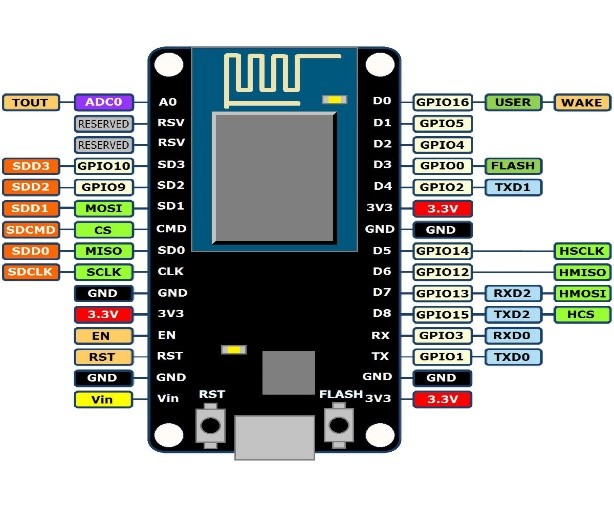
\includegraphics[width=3in]{1}
  \caption{NodeMCU}\label{fig1}
\end{figure}

While writing GPIO code on NodeMCU, you can’t address them with actual GPIO Pin Numbers. There are different I/O Index numbers assigned to each GPIO Pin which is used for GPIO Pin addressing. Figure-2.2 shows a graphical representation of NodeMCU pin settings. Refer following Table \ref{tab1} to check I/O Index of NodeMCU GPIO Pins –

\begin{table}
  \caption{NodeMCU pin settings}\label{tab1}
  \centering
  \begin{tabular}{|p{1in}|p{1.5in}|}
    \hline
    \textbf{GPIO Pin} & I\textbf{/O Index Number}\\[2ex] \hline
    GPIO0 &  3\\[2ex] \hline
    GPIO1 &  10\\[2ex] \hline
    GPIO2 &  4\\[2ex] \hline
    GPIO3 &  9\\[2ex] \hline
    GPIO4 &  2\\[2ex] \hline
    GPIO5 &  1\\[2ex] \hline
    GPIO6 &  N/A\\[2ex] \hline
    GPIO7 &  N/A\\[2ex] \hline
    GPIO8 &  N/A\\[2ex] \hline
    GPIO9 &  11\\[2ex] \hline
    GPIO10 &  12\\[2ex] \hline
    GPIO11 &  N/A\\[2ex] \hline
    GPIO12 &  6\\[2ex] \hline
    GPIO13 &  7\\[2ex] \hline
    GPIO14 &  5\\[2ex] \hline
    GPIO15 &  8\\[2ex] \hline
    GPIO16 &  0\\[2ex] \hline
  \end{tabular}
\end{table}
\newpage

\begin{figure}[t]
  \centering
  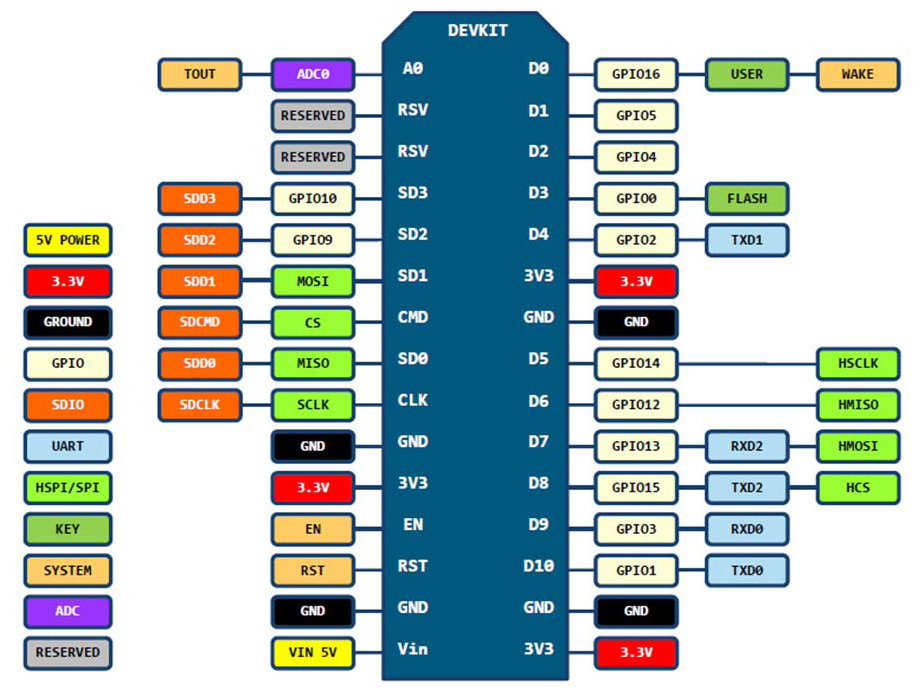
\includegraphics[width=6in]{2}
  \caption{NodeMCU v.1.0 Pin Definition}\label{fig2}
\vspace{.3in}
\end{figure}


The NodeMCU can be programmed with the Arduino software (Arduino IDE). Select "ESP 8266 NodeMCU v.1.0" from the Tools > Board menu. The microcontroller provides pre-burned with a boot loader that allows you to upload new code to it without the use of an external hardware programmer. It communicates using the original STK500 protocol (reference, C header files). It also can bypass the boot loader and program the microcontroller through the ICSP (In-Circuit Serial Programming) header. The NodeMCU has a resettable poly fuse that protects your computer's USB ports from shorts and over current. Although most computers provide their own internal protection, the fuse provides an extra layer of protection. If more than 500mA is applied to the USB port, the fuse will automatically break the connection until the short or overload is removed.\\
\vspace{.3in}
\subsection{Gas sensor MQ-6 Module Specifications}
MQ-6 is a semiconductor type gas sensor which detects the gas leakage. The sensitive material of MQ-6 is tin dioxide (SnO2). It has very low conductivity in clean air. MQ-6 gas sensor has high sensitivity to LPG, concentration level of it is from 200 – 1000 ppm and it also detects the following flammable gases: 1. Propane 2. Hydrogen 3. Methane 4. Butane. Figure \ref{fig3} shows a schematic of MQ-6 gas sensor module [37].\\

\begin{figure}[h]
  \centering
  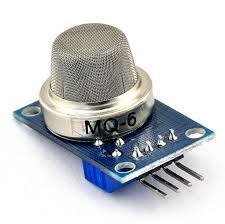
\includegraphics[width=3.6in]{3}
  \caption{MQ-6 Gas sensor}\label{fig3}
\end{figure}

The features of MQ-6 gas sensor are given below:

\begin{enumerate}
  \item Wide detecting scope
\item High sensitivity to combustible gas in wide range
\item Fast response
\item Stable and long life
\item Simple drive circuit
\item Low cost and compact size.
\end{enumerate}

The gas sensor senses the analog value according to the concentration of the gas level in the environment. The concentration range of MQ-6 gas sensor is 200-1000ppm for LPG and use value of Load resistance $(R_L)$ about $20 k\Omega (10 k\Omega to 47 k\Omega)$. When accurately measuring, the proper alarm point for the gas detector should be determined after considering the temperature and humidity influence. The voltage that the sensor outputs changes accordingly to the smoke/gas level that exists in the atmosphere. The sensor outputs a voltage that is proportional to the concentration of smoke/gas. The resistance of the sensor is different depending on the type of the gas. Figure \ref{fig4} shows a schematic of inside circuitry of MQ-6 gas sensor.

\begin{figure}[h]
  \centering
  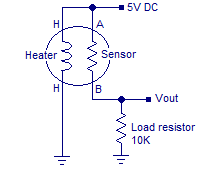
\includegraphics[width=3.5in]{4}
  \caption{MQ-6 circuit.}\label{fig4}
\end{figure}

MQ-6 sensor senses the flammable gases by the increase in temperature when they are oxidized by the heating element. Consider the figure given above. If there is any flammable gas present in the sample, the oxidization of the same gas results in increased temperature and the resistance of the sensor resistor will drop. That means more current will flow through the load resistor and so the voltage across it will shoot up. MQ-6 gas sensor pin description: 1. $D_0$ (Digital Pin), 2. A0 (Analog Pin), 3. VCC (+5V), 4. GND [Graphical illustration in Figure \ref{fig5}].

\begin{figure}[h]
  \centering
  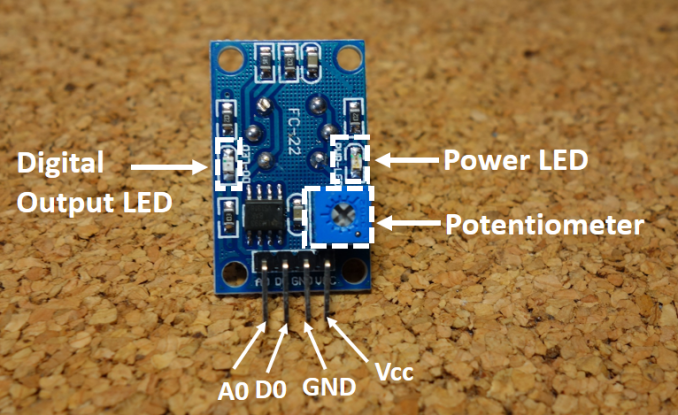
\includegraphics[width=5in]{5}
  \caption{MQ-6 pinout.}\label{fig5}
\end{figure}

The working condition is very important for the sensory performance. Table \ref{tab2} shows the standard working conditions and optimal operations of MQ-6 gas sensor. Sensitivity is also an important factor for the sensory signal calibration. Figure \ref{fig6} and Figure \ref{fig7} shows the sensitive relations of MQ-6 with respect to ppm (Parts per Millions) and Relative Humidity respectively.
\begin{table}[h]
  \caption{Standard Working Condition:}\label{tab2}
  \centering
  \begin{tabular}{|p{.5in}|p{1.5in}|p{1.5in}|p{1.5in}|}
    \hline
    Symbol & Parameter Name & Technical Condition & Remarks\\[1ex] \hline
     $V_C$ & Circuit voltage & $5V\pm0.1$ & AC or DC\\[1ex] \hline
     $V_H$ & Heating voltage & $5V\pm0.1$ & AC or DC\\[1ex] \hline
     $R_L$ & Load resistance & Adjustable & \\[1ex] \hline
     $R_H$ & Heater resistance & $33k.Ohm\pm5\%$ & Room Temperature\\[1ex] \hline
     $P_H$ & Heating consumption & Less than 800mW & \\[1ex]
    \hline
  \end{tabular}
\end{table}
Structure and configuration of MQ-6 gas sensor is shown as Figure\ref{fig6}, sensor composed by micro AL\_2O\_3 ceramic tube, Tin Dioxide (SnO2) sensitive layer, measuring electrode and heater are fixed into a crust made by plastic and stainless steel net. The heater provides necessary work conditions for work of sensitive components. The enveloped MQ-6 have 6 pin ,4 of them are used to fetch signals, and other 2 are used for providing heating current.
\begin{figure}[h]
  \centering
  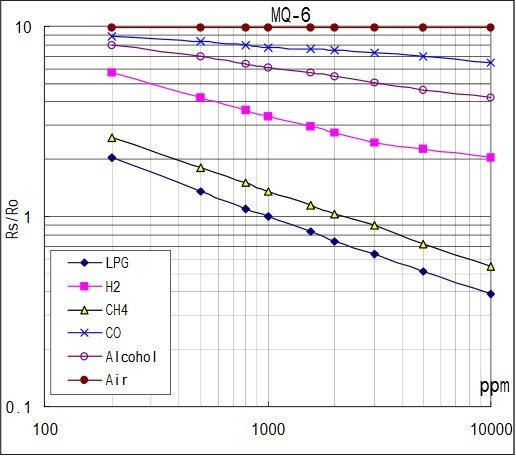
\includegraphics[width=4in]{6}
  \caption{MQ-6 gas sensor sensitivity at optimum conditions [38].}\label{fig6}
\end{figure}
Resistance value of MQ-6 is difference to various kinds and various concentration gases. So, When using this components, sensitivity adjustment is very necessary.Recommend that here calibrated value that detects for 1000 ppm of LPG concentration in air and use value of Load resistance$(R_L)$ about $20 k\Omega (10 k\Omega to 47 k\Omega)$. When accurately measuring, the proper alarm point for the gas detector should be determined after considering the temperature and humidity influence.

\begin{figure}[h]
  \centering
  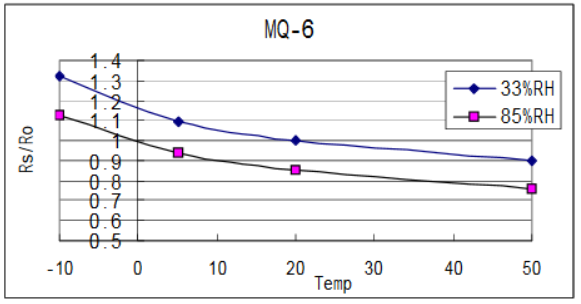
\includegraphics[width=4in]{7}
  \vspace{-.1in}
  \caption{MQ-6 sensor sensitivity with respect to Temperature [38].}\label{fig7}
\end{figure}
Resistance value of MQ-6 is difference to various kinds and various concentration gases. So, when using these components, sensitivity adjustment is very necessary. Recommended that here calibrated value that detects for 1000ppm liquefied petroleum gas (LPG), or 1000ppm iso-butane concentration in air and use value of load resistance that about 20 Kilo-Ohms. When accurately measuring the proper alarm point for the gas detector should be determined after considering the temperature and humidity influence. Applications of MQ-6 gas sensor is given below:
\begin{enumerate}
  \item	Domestic gas leakage detector.
  \item	Industrial combustible gas leakage detector.
  \item	Portable gas leakage detector.
  \item	Concentration level for LPG is 400-1000ppm.
  \item	Circuit voltage is 5V.

\end{enumerate}
\subsection{DHT 11 Humidity \& Temperature Sensor Module Specification}
DHT11 Temperature \& Humidity Sensor features a temperature \& humidity sensor complex with a calibrated digital signal output. By using the exclusive digital-signal-acquisition technique and temperature \& humidity sensing technology, it ensures high reliability and excellent long-term stability. This sensor includes a resistive-type humidity measurement component and an NTC temperature measurement component, and connects to a highperformance 8-bit microcontroller, offering excellent quality, fast response, anti-interference ability and cost-effectiveness.
\begin{figure}[h]
  \centering
  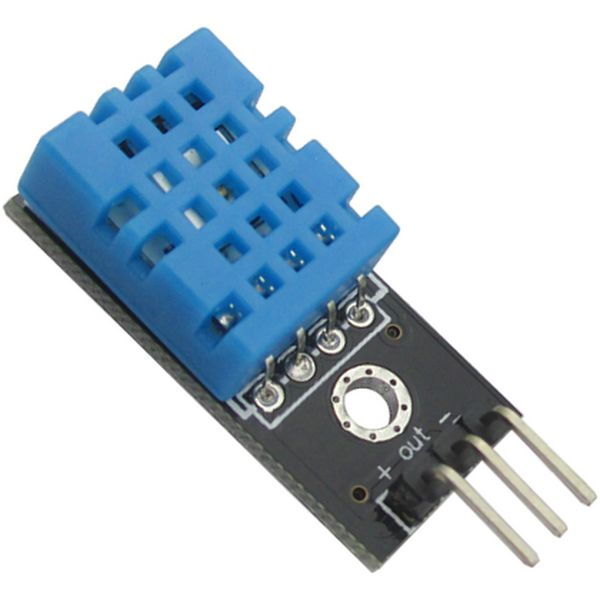
\includegraphics[width=4in]{43}
  \caption{DHT11 Temperature and Humidity sensor Breakout}\label{fig43}
\end{figure}
Each DHT11 element is strictly calibrated in the laboratory that is extremely accurate on humidity calibration. The calibration coefficients are stored as programmes in the OTP memory, which are used by the sensor’s internal signal detecting process\cite{jokar2016intrusion}. The single-wire serial interface makes system integration quick and easy. Its small size, low power consumption and up-to-20 meter signal transmission making it the best choice for various applications, including those most demanding ones. The component is 4-pin single row pin package. It is convenient to
connect and special packages can be provided according to the users.
\newpage
\subsection{DHT11 Temperature \& Humidity Sensor Specification}
\begin{enumerate}
  \item Low cost
\item 3 to 5V power and I/O
\item 2.5mA max current use during conversion (while requesting data)
\item Good for 20-80 \% humidity readings with 5 \% accuracy
\item Good for 0-50 $\circ$ degree C temperature readings $\pm$ 2 $\circ$ degree C accuracy
\item Not more than 1 Hz sampling rate (once every second)
\item Body size 15.5mm x 12mm x 5.5mm
\item 4 pins with 0.1 inch spacing
\end{enumerate}
\subsection{Solenoid Valve Specifications}
\begin{enumerate}
  \item APL-3/2’’-12VDC
  \item	Position: Normally Closed
  \item	Port Size: 1/2" Male NPT
  \item	Voltage: 12V DC
  \item	Body Material: POM Plastic
  \item	Components: Stainless Steel
  \item	Orifice Size: 8.5 mm
  \item	Temp Range: 32 to $125^{\circ}$ F / 0 to $50^{\circ}$C
  \item	Pressure Range: 3 - 115 PSI (Minimum Required)
  \item	Flow Rate: Cv 0.6 (Appx 4.5 GPM @ 60 PSI)
  \item	Power: 6 Watts
\end{enumerate}


Below Figure \ref{fig8} Shows a graphical illustration of 12 V (DC) Solenoid Valve.
\begin{figure}[h]
  \centering
  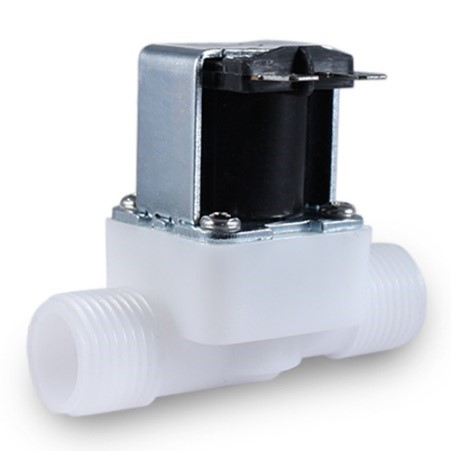
\includegraphics[width=3in]{8}
  \caption{12V DC solenoid valve [39].}\label{fig8}
\end{figure}

\subsection{DC Pump Specification}
\begin{enumerate}
  \item Dimension: 8 x 6 cm
  \item	Brushless pump power: 12V 960mA
  \item	Max water height: 6m
  \item	Max flow: 460LPH
  \item	Lifespan: not less than 20000 hours
  \item	Cable length: 40 cm
  \item	Color: black
  \item	The lead-out wire is 10 cm
  \item	Net weight: 200g
  \item	Package dimension: 88 x 56 x 70 mm
\end{enumerate}

Below Figure \ref{fig9} Shows a graphical illustration of 12 V DC Pump

\begin{figure}[h]
  \centering
  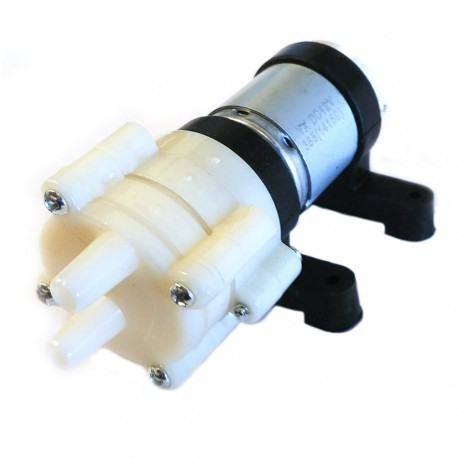
\includegraphics[width=3in]{9}
  \caption{DC Pump}\label{fig9}
\end{figure}

\section{Software Description}
Software tools that are used in the project

\begin{enumerate}
  \item	Arduino IDE (v1.0.6)
  \item	MySQL Database
\end{enumerate}

\subsection{Arduino IDE (v1.0.6)}
The Arduino integrated development environment (IDE) is a cross-platform application written in Java, and derives from the IDE for the Processing programming language and the Wiring projects. It is designed to introduce programming to artists and other newcomers unfamiliar with software development. It includes a code editor with features such as syntax highlighting, brace matching, and automatic indentation, and is also capable of compiling and uploading programs to the board with a single click. A program or code written for Arduino is called a "sketch". Figure \ref{fig10} shows the graphical picture of Arduino-IDE [40].


\begin{figure}[h]
  \centering
  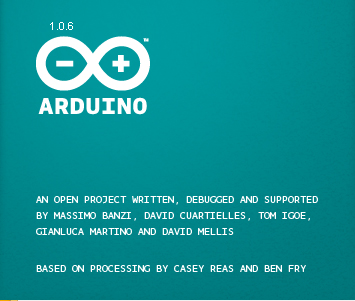
\includegraphics[width=4in]{10}
  \caption{Arduino-IDE lookout}\label{fig10}
\end{figure}

Arduino programs are written in C or C++. The Arduino IDE comes with a software library called "Wiring" from the original Wiring project, which makes many common input/output operations much easier. The users need only to define two functions to make an executable cyclic executive program:

\begin{itemize}
  \item setup(): a function run once at the start of a program that can initialize settings
  \item	loop(): a function called repeatedly until the board powers off
\end{itemize}

A typical first program for a microcontroller simply blinks an LED on and off. In the Arduino environment, the user might write a program like this:

\#define LED\textunderscore PIN 13\\
void setup()\{\\
    pinMode(LED\textunderscore PIN, OUTPUT);~~~~~// Enable pin 13 for digital output\\
\}\\
void loop()\{\\
    digitalWrite(LED\textunderscore PIN, HIGH);~~~~// Turn on the LED\\
    delay(1000);~~~~// Wait one second (1000 milliseconds)\\
    digitalWrite(LED\textunderscore PIN, LOW);~~~~~// Turn off the LED\\
    delay(1000);~~~~~// Wait one second\\
\}\\

It is a feature of most Arduino boards that they have an LED and load resistor connected between pin 13 and ground; a convenient feature for many simple tests. The previous code would not be seen by a standard C++ compiler as a valid program, so when the user clicks the "Upload to I/O board" button in the IDE, a copy of the code is written to a temporary file with an extra include header at the top and a very simple main() function at the bottom, to make it a valid C++ program. The Arduino IDE uses the GNU tool chain and AVR Libc to compile programs, and uses avrdude to upload programs to the board. As the Arduino platform uses Atmel microcontrollers, Atmel's development environment, AVR Studio or the newer Atmel Studio, may also be used to develop software for the Arduino \cite{cohen2018automated}.

\subsection{MySQL database}
MySQL is written in C and C++. Its SQL parser is written in yacc, but it uses a home brewed lexicalanalyzer. MySQLworksonmany systemplatforms,including AIX, BSDi, FreeBSD,HPUX, eComStation, i5/OS, IRIX, Linux, macOS, MicrosoftWindows, NetBSD, Novell,NetWare, OpenBSD, OpenSolaris, OS/2 Warp, QNX, Oracle Solaris, Symbian, SunOS, OpenServer, SCO UnixWare, Sanos and Tru64. A port of MySQL to OpenVMS also exists. The MySQL server software itself and the client libraries use dual-licensing distribution \cite{ercan2017rf}. They are offered under GPL version 2, or a proprietary license. Support can be obtained from the official manual. Free support additionally is available in different IRC channels and forums. Oracle offers paid support via its MySQL Enterprise products. They differ in the scope of services and in price. Additionally, a number of third party organizations exist to provide support and services, including MariaDB and Percona.

\begin{figure}
  \centering
  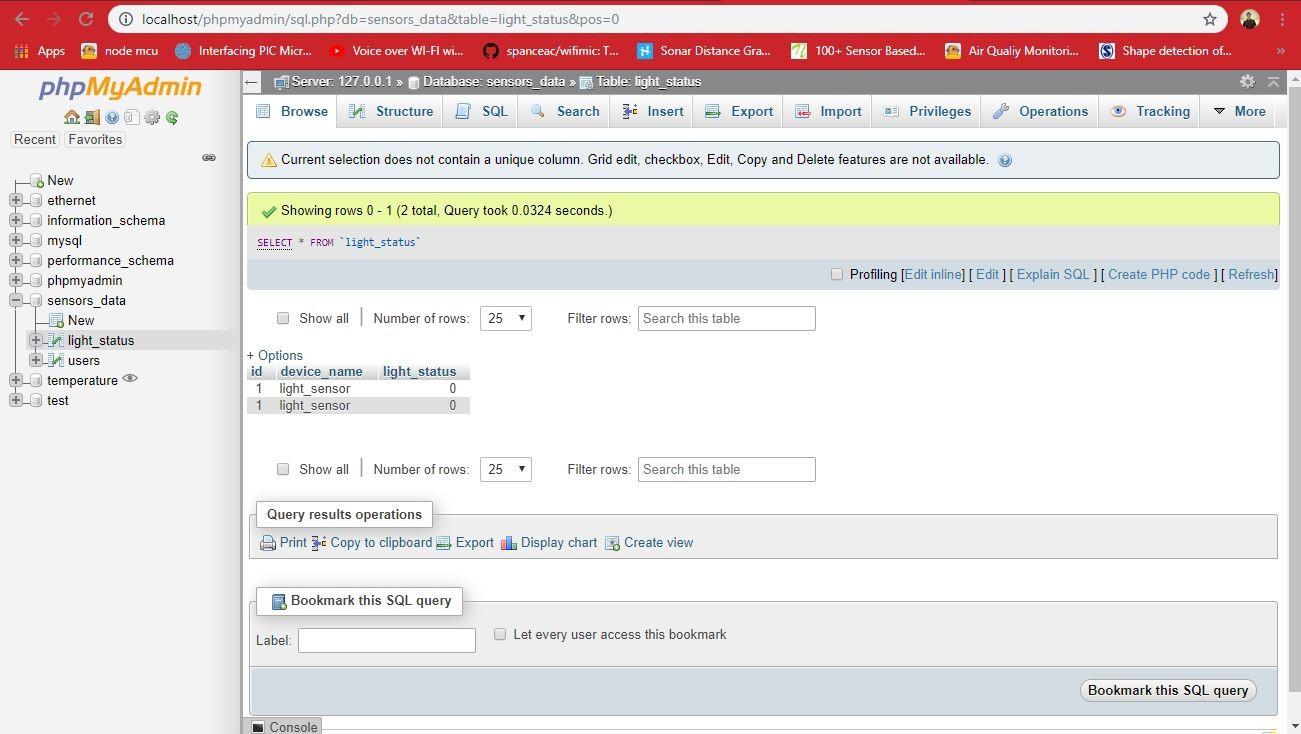
\includegraphics[width=4in,height=2.5 in]{11}
  \caption{Php My Admin console}\label{fig11}
\end{figure}
\section{Chapter Summery}
This chapter contained the details specification of the components used in this project implementation and their power rating.The components were divided into two sections.Every Section contains the proper details about their (components)uses and characteristics. 
\chapter{\textbf{System Methodology}}
A system development methodology refers to the framework that is used to structure, plan, and control the process of developing an information system. Each of the available methodologies is best suited to specific kinds of projects, based on various technical, organizational, project and team considerations.
\section{System Overview}
In this thesis, environment monitoring systems is implemented by using sensors and then send the sensors data are sent to a local internet protocol (IP) using Wi-Fi. For enchanting data, DHT-11 (Temperature and Humidity sensor) and MQ-6 (LPG gas sensor) are being used. The basic objective of this work is to monitor and to develop a real-time monitoring of humidity and temperature, as well as the availability of gas using the very available DHT-11 sensor, MQ-6 sensor, and ESP-8266 NodeMCU module and then observe the data from a local IP based webpage. In this, a system has been developed to monitor the real-time condition (Humidity and Temperature to be more precise) through a local IP without the access of internet, because of security reason and so on; in which physical presence is not needed.
\begin{figure}[h]
\vspace{.5in}
  \centering
  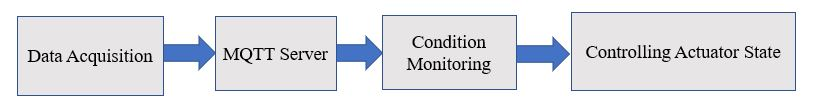
\includegraphics[width=6in]{12}
  \caption{ System Block Diagram}\label{fig12}
  \vspace{.5in}
\end{figure}
Node MCU is a kind of component that consists of an ESP8266 Wi-Fi along with a microcontroller with 1 analog and 12 digital pins, for which it is more efficient than an Arduino board and the data rate is also effective for this module. Combining the results with MATLAB environment, the upcoming data can also be forecasted through the basic knowledge of MATLAB or other engineering and scientific software. However, using an Arduino board is not necessary for just monitoring services, because of cost management and time consumption. This work has been directed using very modest methodology and appliances which are available and require minimal technical knowledge to operate. It discusses one of the implementations of a system using Wireless Sensor Networking (WSN). MQ-2 gas sensor and IR photodiode are used to determine smoke/gas concentration and fire presence respectively. As the gas sensor works fine within temperature ranging 2535 0C \& RH ranging 55-70\%, so DHT-11 sensor is used to check the temperature and relative humidity level of the experimental plant. Further mathematical modeling and analysis are done for the steady-state design of the experimental system. After that acquisition of those factors which combines a threshold, value has to be set for controlling the total system modeling. From the datasheet of DHT-11, MQ-2 and IR photodiode, parameters and the operations are obtained. The DHT-11 sensor is a digital sensor with digital output data, which combines Integrated Circuits, is the reason behind the direct values of relative humidity and temperature can be obtained.

\section{Why ESP8266 is Used}
In this project work we have used ESP8266 as MCU because of the following reasons:\\\\
\textbf{(i)Ideal Stuff for IoT and WSN:} ESP8266 is ideal for Internet of Things (IoT) My current project involves home automation and IoT stuff. It would send the status of a PIR Sensor over WIFI to an MQTT broker every 2.5 seconds. With built-in WIFI, these boards are ideal for Internet activities.\\\\
\textbf{(ii)Programmable PWM Frequency:} The ESP8266 core of the Arduino library, however, has a built-in PWM frequency call. The ESP8266 core has 1024 (0-1023) levels of pulse-width instead of Arduino’s 256 (0-255). One option is to change the PWM frequency, but that would mean digging in the Arduino libraries.\\\\
\textbf{(iii)Any pins can be selected for I2C:} A simple call before initializing the wire library allows for I2C communication on any of the module’s pins.\\\\
\textbf{(iv)Works with Arduino IDE:} The reason for choosing this is that the ESP8266 works well with the Arduino IDE.\\\\
\textbf{(v)Inexpensive:} The Adafruit ESP8266 boards have incredible build quality, nice features (like all the necessary pull-ups), and support a company that supports the maker community in countless ways. Moreover, it is cheap in price.

\section{System Flowchart}
Firstly, when the Node MCU is turned, it first runs the program compiled in it and starts calibrating the sensors. On concluding calibration, it first goes to connect the local server via triggering its Tx and Rx. Now, two types of conditions are relevant; at calibration, the controller detects any problem in sensor value then it sends a signal to the control unit and commands it to make an action. Next, it starts recalibration and if no defect is found then it tries to connect the hotspot which is specified in the program and it checks for the preprogrammed SSID and if found nearby then the connection is created and an IP address is obtained. After connecting to the internet, it tries to connect with the prespecified Local IP. Then the controller creates a data transmission network between the sensors and the IP. Data from the sensor are transferred to the server. The system flowchart is shown in Figure \ref{fig13}

\begin{figure}
  \centering
  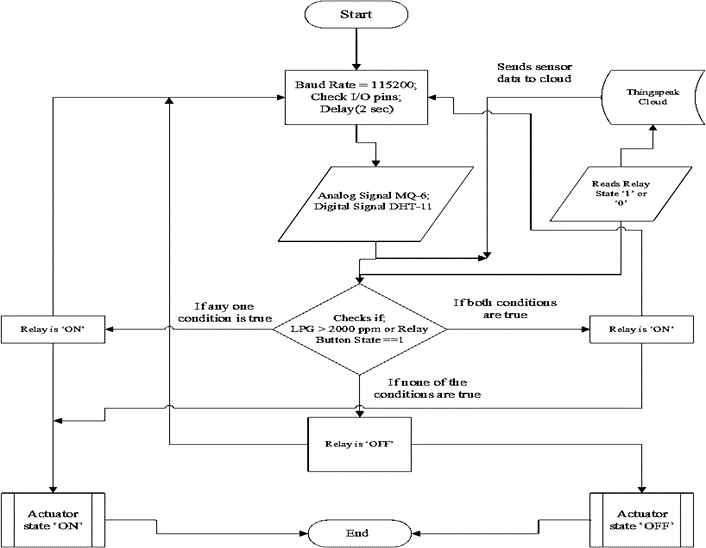
\includegraphics[width=6in,height=6in]{13}
  \caption{Flowchart of the monitoring system}\label{fig13}
\end{figure}
\section{Chapter Summery}
This chapter is about the methods and the algorithm which was used for the system implementation.This chapter contains flowchart with formalized graphic representation of a logic sequence, work process and formalized structure. The purpose of a flow chart is to provide people with a common language or reference point when dealing with a project or process.This Chapter reflects all of this.    
\chapter{\textbf{Mathematical Modeling}}
As the system focuses on gas concentration-based alerting and control of appliances, thus only MQ-6 gas sensor calibration is considered for the mathematical analysis. DHT-11 sensor is to for checking the conditional Temperature and Relative Humidity.

\begin{figure}[h]
  \centering
  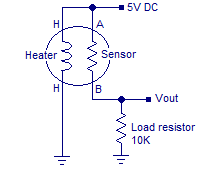
\includegraphics[width=2in]{14}
  \caption{MQ-6 Equivalent Circuit.}\label{fig14}
\end{figure}

\begin{justify}
Let, V\textsubscript{C} = Supply Voltage = +5V
\end{justify}\par

\begin{justify}
R\textsubscript{S} = Sensor Resistance
\end{justify}\par

\begin{justify}
R\textsubscript{L} = Load Resistance (Variable)
\end{justify}\par

\begin{justify}
V\textsubscript{out} = Sensor output Voltage
\end{justify}\par

\begin{justify}
From, Current flow and Voltage relationship,\ \ \ \ \ \ \ \ \ \ \ \ \ \ \ \ \ \ \ \ \ \ \ \ \ \ \ \ \ \ \ \ \ \
\end{justify}\par

\begin{equation}\label{5.1}
  V=I \times R
\end{equation}

\begin{equation*}
  ( V_{out}=\frac{Analog value \times 5}{1023})
\end{equation*}


Resistance of the sensor () is defined in datasheet [38] of MQ-6 as:\par

\begin{equation}\label{5.2}
  R_{s}= \left( \frac{V_{cc}}{V_{out}}-1 \right)  \times R_{L}= \left( \frac{1023}{Analog value}-1 \right)  \times R_{L}
\end{equation}

\vspace{\baselineskip}
Fresh air resistance ration for gas sensors: [38]\par

\begin{justify}
Data analyzing from R\textsubscript{S}/R\textsubscript{0} vs ppm graph: From the equations of a straight line,
\end{justify}\par



%%%%%%%%%%%%%%%%%%%% Table No: 1 starts here %%%%%%%%%%%%%%%%%%%%

\begin{equation}\label{5.3}
  y=mx+b
\end{equation}


%%%%%%%%%%%%%%%%%%%% Table No: 1 ends here %%%%%%%%%%%%%%%%%%%%

\begin{justify}
Here, y = value on Y-axis; x = value on X-axis; m = Slope of line; b = Intercept from Y-axis
\end{justify}\par

\begin{justify}
For log-log plot equation-(5) becomes:
\end{justify}\par


\begin{equation}\tag{5.4}
log \left( y \right) =m \times log \left( x \right) +b
\end{equation}
\begin{justify}
Note: the log is base 10.
\end{justify}\par

\begin{justify}
Slope (m) Value formula: If (x\textsubscript{0}, y\textsubscript{0}) and (x, y) are any two points of a line from a log-log plot then the formula for determining m is below:
\end{justify}\par


\begin{equation}\tag{5.5}
m=\frac{log_{10} \left( \frac{y}{y_{0}} \right) }{log_{10} \left( \frac{x}{x_{0}} \right) }
\end{equation}
\begin{justify}
Intercept from Y-axis (b) Value formula:
\end{justify}\par

\begin{justify}
From, equation-(5.6);
\end{justify}\par

\begin{equation*}
 ( log_{10} \left( y \right) =m \times log_{10} \left( x \right) +b)
\end{equation*}


\begin{equation}\tag{5.6}
Or, b=log_{10} \left( y \right) -m \times log_{10} \left( x \right)
\end{equation}
\begin{justify}
Using equations-(1) to (8) the gas concentration can be\textbf{ }determined directly in ppm (Parts per millions)
\end{justify}\par


\begin{equation}\tag{5.7}
log_{10} \left( ppm \right) =\frac{ \left( log_{10} \left( \frac{R_{s}}{R_{0}} \right) -b \right) }{m}
\end{equation}
From the MQ-6 datasheet we have obtained the value of m and b from equation (5.5) and (5.6)\par

\setlength{\parskip}{0.0pt}
Slope, m  \( = -0.423 \) \  \par

And b  \( =1.276 \)  \par

And sensor resistance  \( R_{0} \) =5.62  \( k \Omega  \) \par


\vspace{\baselineskip}
\setlength{\parskip}{8.04pt}
\par


\vspace{\baselineskip}
\setlength{\parskip}{0.0pt}


%%%%%%%%%%%%%%%%%%%% Table No: 2 starts here %%%%%%%%%%%%%%%%%%%%


\begin{table}[H]
\caption{Raw voltage values received through the MQ-6 sensor and corresponding temperature and humidity values:}
 			\centering
\begin{tabular}{p{0.23in}p{1.24in}p{1.55in}p{1.18in}p{1.37in}}
\hline
%row no:1
\multicolumn{1}{|p{0.23in}}{\Centering ID} &
\multicolumn{1}{|p{1.24in}}{\Centering Time} &
\multicolumn{1}{|p{1.55in}}{\Centering Temperature (in $ ^{\circ} $ C)} &
\multicolumn{1}{|p{1.18in}}{\Centering Humidity (in $\%$ )} &
\multicolumn{1}{|p{1.37in}|}{\Centering Analog value} \\
\hhline{-----}
%row no:2
\multicolumn{1}{|p{0.23in}}{\Centering 1} &
\multicolumn{1}{|p{1.24in}}{\Centering 13:19:41} &
\multicolumn{1}{|p{1.55in}}{\Centering 30} &
\multicolumn{1}{|p{1.18in}}{\Centering 61} &
\multicolumn{1}{|p{1.37in}|}{\Centering 533.15} \\
\hhline{-----}
%row no:3
\multicolumn{1}{|p{0.23in}}{\Centering 2} &
\multicolumn{1}{|p{1.24in}}{\Centering 13:19:36} &
\multicolumn{1}{|p{1.55in}}{\Centering 30} &
\multicolumn{1}{|p{1.18in}}{\Centering 61} &
\multicolumn{1}{|p{1.37in}|}{\Centering 533.48} \\
\hhline{-----}
%row no:4
\multicolumn{1}{|p{0.23in}}{\Centering 3} &
\multicolumn{1}{|p{1.24in}}{\Centering 13:19:31} &
\multicolumn{1}{|p{1.55in}}{\Centering 30} &
\multicolumn{1}{|p{1.18in}}{\Centering 61} &
\multicolumn{1}{|p{1.37in}|}{\Centering 532.48} \\
\hhline{-----}
%row no:5
\multicolumn{1}{|p{0.23in}}{\Centering 4} &
\multicolumn{1}{|p{1.24in}}{\Centering 13:19:25} &
\multicolumn{1}{|p{1.55in}}{\Centering 30} &
\multicolumn{1}{|p{1.18in}}{\Centering 61} &
\multicolumn{1}{|p{1.37in}|}{\Centering 528.04} \\
\hhline{-----}
%row no:6
\multicolumn{1}{|p{0.23in}}{\Centering 5} &
\multicolumn{1}{|p{1.24in}}{\Centering 13:19:20} &
\multicolumn{1}{|p{1.55in}}{\Centering 30} &
\multicolumn{1}{|p{1.18in}}{\Centering 61} &
\multicolumn{1}{|p{1.37in}|}{\Centering 532.48} \\
\hhline{-----}
%row no:7
\multicolumn{1}{|p{0.23in}}{\Centering 6} &
\multicolumn{1}{|p{1.24in}}{\Centering 13:19:15} &
\multicolumn{1}{|p{1.55in}}{\Centering 30} &
\multicolumn{1}{|p{1.18in}}{\Centering 61} &
\multicolumn{1}{|p{1.37in}|}{\Centering 532.48} \\
\hhline{-----}
%row no:8
\multicolumn{1}{|p{0.23in}}{\Centering 7} &
\multicolumn{1}{|p{1.24in}}{\Centering 13:19:10} &
\multicolumn{1}{|p{1.55in}}{\Centering 30} &
\multicolumn{1}{|p{1.18in}}{\Centering 61} &
\multicolumn{1}{|p{1.37in}|}{\Centering 528.04} \\
\hhline{-----}
%row no:9
\multicolumn{1}{|p{0.23in}}{\Centering 8} &
\multicolumn{1}{|p{1.24in}}{\Centering 13:19:05} &
\multicolumn{1}{|p{1.55in}}{\Centering 30} &
\multicolumn{1}{|p{1.18in}}{\Centering 61} &
\multicolumn{1}{|p{1.37in}|}{\Centering 528.04} \\
\hhline{-----}
%row no:10
\multicolumn{1}{|p{0.23in}}{\Centering 9} &
\multicolumn{1}{|p{1.24in}}{\Centering 13:18:59} &
\multicolumn{1}{|p{1.55in}}{\Centering 30} &
\multicolumn{1}{|p{1.18in}}{\Centering 61} &
\multicolumn{1}{|p{1.37in}|}{\Centering 528.04} \\
\hhline{-----}
%row no:11
\multicolumn{1}{|p{0.23in}}{\Centering 10} &
\multicolumn{1}{|p{1.24in}}{\Centering 13:18:54} &
\multicolumn{1}{|p{1.55in}}{\Centering 30} &
\multicolumn{1}{|p{1.18in}}{\Centering 61} &
\multicolumn{1}{|p{1.37in}|}{\Centering 528.04} \\
\hhline{-----}

\end{tabular}
 \end{table}


%%%%%%%%%%%%%%%%%%%% Table No: 2 ends here %%%%%%%%%%%%%%%%%%%%


\vspace{\baselineskip}
\setlength{\parskip}{8.04pt}
\par



%%%%%%%%%%%%%%%%%%%% Table No: 3 starts here %%%%%%%%%%%%%%%%%%%%


\begin{table}[H]
\caption{The Temperature and Humidity correction factor is used and the Corrected Resistance and subsequently the Corrected PPM is evaluated: [69]}
\label{tab:5. 3 The Temperature and Humidity correction factor is used and the Corrected Resistance and subsequently the Corrected PPM is evaluated: [69]}
 			\centering
\begin{tabular}{p{0.23in}p{1.24in}p{1.55in}p{2.74in}}
\hline
%row no:1
\multicolumn{1}{|p{0.23in}}{\Centering ID} &
\multicolumn{1}{|p{1.24in}}{\Centering Time} &
\multicolumn{1}{|p{1.55in}}{\Centering Resistance ( \( R_{s} \) )} &
\multicolumn{1}{|p{2.74in}|}{\Centering PPM} \\
\hhline{----}
%row no:2
\multicolumn{1}{|p{0.23in}}{\Centering 1} &
\multicolumn{1}{|p{1.24in}}{\Centering 13:19:41} &
\multicolumn{1}{|p{1.55in}}{\Centering 9187.764} &
\multicolumn{1}{|p{2.74in}|}{\Centering 325} \\
\hhline{----}
%row no:3
\multicolumn{1}{|p{0.23in}}{\Centering 2} &
\multicolumn{1}{|p{1.24in}}{\Centering 13:19:36} &
\multicolumn{1}{|p{1.55in}}{\Centering 9175.828} &
\multicolumn{1}{|p{2.74in}|}{\Centering 316} \\
\hhline{----}
%row no:4
\multicolumn{1}{|p{0.23in}}{\Centering 3} &
\multicolumn{1}{|p{1.24in}}{\Centering 13:19:31} &
\multicolumn{1}{|p{1.55in}}{\Centering 9211.781} &
\multicolumn{1}{|p{2.74in}|}{\Centering 313} \\
\hhline{----}
%row no:5
\multicolumn{1}{|p{0.23in}}{\Centering 4} &
\multicolumn{1}{|p{1.24in}}{\Centering 13:19:25} &
\multicolumn{1}{|p{1.55in}}{\Centering 9373.252} &
\multicolumn{1}{|p{2.74in}|}{\Centering 310} \\
\hhline{----}
%row no:6
\multicolumn{1}{|p{0.23in}}{\Centering 5} &
\multicolumn{1}{|p{1.24in}}{\Centering 13:19:20} &
\multicolumn{1}{|p{1.55in}}{\Centering 9211.781} &
\multicolumn{1}{|p{2.74in}|}{\Centering 313} \\
\hhline{----}
%row no:7
\multicolumn{1}{|p{0.23in}}{\Centering 6} &
\multicolumn{1}{|p{1.24in}}{\Centering 13:19:15} &
\multicolumn{1}{|p{1.55in}}{\Centering 9211.781} &
\multicolumn{1}{|p{2.74in}|}{\Centering 313} \\
\hhline{----}
%row no:8
\multicolumn{1}{|p{0.23in}}{\Centering 7} &
\multicolumn{1}{|p{1.24in}}{\Centering 13:19:10} &
\multicolumn{1}{|p{1.55in}}{\Centering 9373.252} &
\multicolumn{1}{|p{2.74in}|}{\Centering 310} \\
\hhline{----}
%row no:9
\multicolumn{1}{|p{0.23in}}{\Centering 8} &
\multicolumn{1}{|p{1.24in}}{\Centering 13:19:05} &
\multicolumn{1}{|p{1.55in}}{\Centering 9373.252} &
\multicolumn{1}{|p{2.74in}|}{\Centering 310} \\
\hhline{----}
%row no:10
\multicolumn{1}{|p{0.23in}}{\Centering 9} &
\multicolumn{1}{|p{1.24in}}{\Centering 13:18:59} &
\multicolumn{1}{|p{1.55in}}{\Centering 9373.252} &
\multicolumn{1}{|p{2.74in}|}{\Centering 310} \\
\hhline{----}
%row no:11
\multicolumn{1}{|p{0.23in}}{\Centering 10} &
\multicolumn{1}{|p{1.24in}}{\Centering 13:18:54} &
\multicolumn{1}{|p{1.55in}}{\Centering 9373.252} &
\multicolumn{1}{|p{2.74in}|}{\Centering 310} \\
\hhline{----}

\end{tabular}
 \end{table}


%%%%%%%%%%%%%%%%%%%% Table No: 3 ends here %%%%%%%%%%%%%%%%%%%%


\vspace{\baselineskip}
\par


\begin{equation}\tag{5.8}
R_{s} \_ Scaling factor=1.6979-0.012t-0.00612h
\end{equation}
\begin{equation*}
   (  Corrected R_{s}= \frac{R_{s}}{R_{s} \_ Scaling factor})
\end{equation*}




%%%%%%%%%%%%%%%%%%%% Table No: 4 starts here %%%%%%%%%%%%%%%%%%%%


\begin{table}[H]
\caption{The Temperature and Humidity correction factor is used and the Corrected Resistance and subsequently the Corrected PPM is evaluated: [69]}
 			\centering
\begin{tabular}{p{0.23in}p{1.24in}p{1.68in}p{1.05in}p{1.37in}}
\hline
%row no:1
\multicolumn{1}{|p{0.23in}}{\Centering ID} &
\multicolumn{1}{|p{1.24in}}{\Centering Time} &
\multicolumn{1}{|p{1.68in}}{\Centering Resistance Corrected  \( R_{s} \) } &
\multicolumn{1}{|p{1.05in}}{\Centering Corrected PPM} &
\multicolumn{1}{|p{1.37in}|}{\Centering Correction Factor} \\
\hhline{-----}
%row no:2
\multicolumn{1}{|p{0.23in}}{\Centering 1} &
\multicolumn{1}{|p{1.24in}}{\Centering 13:19:41} &
\multicolumn{1}{|p{1.68in}}{\Centering 7177.940} &
\multicolumn{1}{|p{1.05in}}{\Centering 582.55} &
\multicolumn{1}{|p{1.37in}|}{\Centering 1.28} \\
\hhline{-----}
%row no:3
\multicolumn{1}{|p{0.23in}}{\Centering 2} &
\multicolumn{1}{|p{1.24in}}{\Centering 13:19:36} &
\multicolumn{1}{|p{1.68in}}{\Centering 7168.615} &
\multicolumn{1}{|p{1.05in}}{\Centering 584.34} &
\multicolumn{1}{|p{1.37in}|}{\Centering 1.28} \\
\hhline{-----}
%row no:4
\multicolumn{1}{|p{0.23in}}{\Centering 3} &
\multicolumn{1}{|p{1.24in}}{\Centering 13:19:31} &
\multicolumn{1}{|p{1.68in}}{\Centering 7196.703} &
\multicolumn{1}{|p{1.05in}}{\Centering 578.96} &
\multicolumn{1}{|p{1.37in}|}{\Centering 1.28} \\
\hhline{-----}
%row no:5
\multicolumn{1}{|p{0.23in}}{\Centering 4} &
\multicolumn{1}{|p{1.24in}}{\Centering 13:19:25} &
\multicolumn{1}{|p{1.68in}}{\Centering 7338.478} &
\multicolumn{1}{|p{1.05in}}{\Centering 552.87} &
\multicolumn{1}{|p{1.37in}|}{\Centering 1.28} \\
\hhline{-----}
%row no:6
\multicolumn{1}{|p{0.23in}}{\Centering 5} &
\multicolumn{1}{|p{1.24in}}{\Centering 13:19:20} &
\multicolumn{1}{|p{1.68in}}{\Centering 7196.703} &
\multicolumn{1}{|p{1.05in}}{\Centering 578.96} &
\multicolumn{1}{|p{1.37in}|}{\Centering 1.28} \\
\hhline{-----}
%row no:7
\multicolumn{1}{|p{0.23in}}{\Centering 6} &
\multicolumn{1}{|p{1.24in}}{\Centering 13:19:15} &
\multicolumn{1}{|p{1.68in}}{\Centering 7196.703} &
\multicolumn{1}{|p{1.05in}}{\Centering 578.96} &
\multicolumn{1}{|p{1.37in}|}{\Centering 1.28} \\
\hhline{-----}
%row no:8
\multicolumn{1}{|p{0.23in}}{\Centering 7} &
\multicolumn{1}{|p{1.24in}}{\Centering 13:19:10} &
\multicolumn{1}{|p{1.68in}}{\Centering 7338.478} &
\multicolumn{1}{|p{1.05in}}{\Centering 552.87} &
\multicolumn{1}{|p{1.37in}|}{\Centering 1.28} \\
\hhline{-----}
%row no:9
\multicolumn{1}{|p{0.23in}}{\Centering 8} &
\multicolumn{1}{|p{1.24in}}{\Centering 13:19:05} &
\multicolumn{1}{|p{1.68in}}{\Centering 7338.478} &
\multicolumn{1}{|p{1.05in}}{\Centering 552.87} &
\multicolumn{1}{|p{1.37in}|}{\Centering 1.28} \\
\hhline{-----}
%row no:10
\multicolumn{1}{|p{0.23in}}{\Centering 9} &
\multicolumn{1}{|p{1.24in}}{\Centering 13:18:59} &
\multicolumn{1}{|p{1.68in}}{\Centering 7338.478} &
\multicolumn{1}{|p{1.05in}}{\Centering 552.87} &
\multicolumn{1}{|p{1.37in}|}{\Centering 1.28} \\
\hhline{-----}
%row no:11
\multicolumn{1}{|p{0.23in}}{\Centering 10} &
\multicolumn{1}{|p{1.24in}}{\Centering 13:18:54} &
\multicolumn{1}{|p{1.68in}}{\Centering 7338.478} &
\multicolumn{1}{|p{1.05in}}{\Centering 552.87} &
\multicolumn{1}{|p{1.37in}|}{\Centering 1.28} \\
\hhline{-----}

\end{tabular}
 \end{table}


%%%%%%%%%%%%%%%%%%%% Table No: 4 ends here %%%%%%%%%%%%%%%%%%%%



\section{Algorithm of the process }
\setlength{\parskip}{0.0pt}
\textcolor[HTML]{111111}{setup( )}\par

\textcolor[HTML]{111111}{$ \{ $  setAnalogPinforMQ135(analog0);}\par

\textcolor[HTML]{111111}{setAnalogP}\par

\textcolor[HTML]{111111}{inforDHT11(analog1);}\par

\textcolor[HTML]{111111}{Serial.begin(9600);}\par

\textcolor[HTML]{111111}{$ \} $ }\par

\textcolor[HTML]{111111}{loop( )}\par

\textcolor[HTML]{111111}{$ \{ $ \  AnalogValue = receiveMQdata( );}\par

T = TempfromDHT11( );\par

H = HumfromDHT11( );\par

Vout= convertanalogtovoltage(AnalogValue);\par

while(calibrationisnotcomplete)\par

$ \{ $  RO= calculateRoValue(Vout, DefaultPPM);$ \} $ \par

RS= calculateRsValue(CaliberatedRO, Vout);\par

CorrectedRS= TempHumCalibRs(RS, T, H);\par

ppm = PPM(RS, RO, MQ\_Scaling\_Factor, MQ\_Exponent\_Factor); \par

Correctedppm = PPM(CorrectedRS, RO, MQ\_Scaling\_Factor, MQ\_Exponent\_Factor);\par

PlotDatainMatlab( );\par

SendDatatoSerialMonitor( );\par

SendDatatoExcel( );\par

$ \} $ \par

\setlength{\parskip}{8.04pt}
\section{Calculation of the solar PV energy output of a photovoltaic cell [70]}
\begin{justify}
We construct a solar panel which is used for powering the controller. A dimension about 11.5cm \(   \times  \)  6 cm rectangular solar plate is used to make the solar panel.
\end{justify}\par



%%%%%%%%%%%%%%%%%%%% Table No: 5 starts here %%%%%%%%%%%%%%%%%%%%

%
%\begin{table}[H]
% 			\centering
%\begin{tabular}{p{1.69in}p{1.6in}p{2.8in}}
%%row no:1
%\multicolumn{1}{p{1.69in}}{\textbf{Global formula:}} &
%\multicolumn{1}{p{1.6in}}{ \( E=A \times r \times H \times PR \) \ \  } &
%\multicolumn{1}{p{2.8in}}{(5.9)} \\
%\hhline{~~~}
%
%\end{tabular}
% \end{table}
 \begin{equation}\tag{5.9}
\textbf{Global formula}:Energy,E=A \times r \times H \times PR
\end{equation}


%%%%%%%%%%%%%%%%%%%% Table No: 5 ends here %%%%%%%%%%%%%%%%%%%%


\vspace{\baselineskip}


%%%%%%%%%%%%%%%%%%%% Table No: 6 starts here %%%%%%%%%%%%%%%%%%%%


\begin{table}[H]
 			\centering
\begin{tabular}{p{5.13in}p{1.15in}}
\hline
%row no:1
\multicolumn{1}{|p{5.13in}}{E = Energy (kWh)\ \  \ \ \ \ \ \ \ \ \  } &
\multicolumn{1}{|p{1.15in}|}{ kWh/an} \\
\hhline{--}
%row no:2
\multicolumn{1}{|p{5.13in}}{A = Total solar panel Area $(m^2)$} &
\multicolumn{1}{|p{1.15in}|}{0.0069 $m^2$} \\
\hhline{--}
%row no:3
\multicolumn{1}{|p{5.13in}}{r = solar panel yield ($\%$ )} &
\multicolumn{1}{|p{1.15in}|}{15$\%$ } \\
\hhline{--}
%row no:4
\multicolumn{1}{|p{5.13in}}{H = Annual average irradiation on tilted panel (shadings not included) $\ast$ } &
\multicolumn{1}{|p{1.15in}|}{ $kWh/m^2.an$} \\
\hhline{--}
%row no:5
\multicolumn{1}{|p{5.13in}}{PR = Performance ratio, coefficient for losses (range between 0.9 and 0.5, default value =0.75)} &
\multicolumn{1}{|p{1.15in}|}{0.75} \\
\hhline{--}

\end{tabular}
 \end{table}


%%%%%%%%%%%%%%%%%%%% Table No: 6 ends here %%%%%%%%%%%%%%%%%%%%


\vspace{\baselineskip}
\section{Relative Humidity Calculation using DHT11 Sensor}

After getting start pulse from the controller, DHT11 sends the response pulse to the microcontroller which will indicate that DHT11 received start pulse.The response pulse is low for 54 microsecond and then goes high for 80 microsecond.
After sending the response pulse, DHT11 sensor sends the data, which contains humidity and temperature value along with checksum. The data frame is of total 40 bits long, it contains 5 segments (byte) and each segment is 8-bit long.In this 5 segments first two segments content humidity value in decimal integer form. This Value gives  Relative Percentage Humidity. 1st 8-bits are integer part and next 8 bits are fractional partNext two segment content temperature value in decimal integer form. This value gives us temperature in Celsius form.
Here checksum byte is direct addition of humidity and temperature value. And it would be verified using it in microcontroller whether it is same as checksum value or not. If it is not equal, then there is some error in the data value otherwise the data is correct.Once microcontroller receives data, DHT11 pin goes in low power consumption mode until the microcontroller do not sends start pulse again \cite{collotta2018bluetooth}.

\textbf{End-Pulse}:After sending 40-bit data, DHT11 sensor sends 54us low level and then goes high. After this DHT11 goes in sleep mode.
If the temperature and the dewpoint was knew, and wanted to obtain relative humidity, the formulas are as follows:\par
First, to convert the temperature and the dewpoint from Fahrenheit to Celsius, use the following formulas.\par

\begin{equation}\tag{5.10}
 T_{c}=\frac{5 \times  \left( T_{f}-32.0 \right) }{9}
\end{equation}

\begin{equation}\tag{5.11}
T_{dc}=\frac{5 \times  \left( T_{df}-32.0 \right) }{9}
\end{equation}
 \( T_{c} \) =air temperature in degrees Celsius,  \( T_{f} \) =air temperature in degrees Fahrenheit\par

 \( T_{dc} \) =dewpoint temperature in degrees Celsius\par

 \( T_{df} \) =dewpoint temperature in degrees Fahrenheit\par

The next set of formulas assumes a standard atmospheric pressure. These formulas will calculate saturation vapor pressure (Es) and actual vapor pressure(E) in millibars.\par


\begin{equation}\tag{5.12}
E_{s}=6.11 \times 10.0  \times  \left( \frac{7.5 \times T_{c}}{237.7+T_{c}} \right)
\end{equation}

\vspace{\baselineskip}
\setlength{\parskip}{0.0pt}

\begin{equation}\tag{5.13}
E=6.11 \times 10.0  \times  \left( \frac{7.5 \times T_{dc}}{237.7+T_{dc}} \right) \ \ \
\end{equation}
Once the saturation vapor pressure and the actual vapor pressure, relative humidity can be computed by dividing the actual vapor pressure by the saturation vapor pressure and then multiplying by 100 to convert the quantity to a percent.\par


\begin{equation}\tag{5.14}
Relative Humidity (RH) in percent =\frac{E}{E_{s}} \times 100\%
\end{equation}
For example, a station report that included an air temperature of 85 degrees Fahrenheit and a dewpoint of 65 degrees Fahrenheit and you wanted to compute the relative humidity, you would proceed as follows \cite{schafer2013accurate}.\\

First, convert the Fahrenheit values to Celsius using formulas. The values should be  \( T_{c} \) =29.4 and  \( T_{dc} \) =18.3\par

Next, calculate the saturation vapor pressure and the actual vapor pressure using formulas (5.12) and (5.13) respectively. The values should be  \( E_{s} \)  =40.9 and  \( E \)  =21.0\par

Finally, calculate relative humidity using formula (5.14). The final answer should be RH=51.3 $\%$ .\par
\section{Chapter Summery}
In this Chapter mathematical modelling of the sensor was derived and by using this calculation the analog voltage of the Gas sensor is converted into the PPM value as well as the temperature and the humidity also calculated using above described equations.This chapter also contains the solar equivalent energy which is provided to the controller for supplying power.  
\chapter{\textbf{Experimental Setup}}
Wireless sensor networks (WSNs) are networks of interconnected wireless devices that are embedded into the physical environment to provide measurements of many points over large spaces. These devices have built-in processing, storage, and radio frequency sensors and antennas. They are linked into an interconnected network that routes the data they capture to a computer for analysis.\\
Environmental protection is one of the most challenging tasks for humanity. All of the latest technologies to certain extent are applied in this area, among others, wireless sensor networks as well. In this paper a wireless sensor node designed specifically for monitoring of environmental parameters is described. The main advantage of this node is the use of energy harvesting techniques and supercapacitor as power supply method. The absence of batteries affects the reduction of maintenance costs and environmental impact. The paper shows that combination of energy harvesting and supercapacitor represents a sustainable solution of constant power supply of wireless sensor network node.
The WSN has one or more sensor node. These sensor nodes are used to extract data from the environment of the home. A Router is used to develop local IP based web server. It will provide a muscular networking mechanism over comfortable range of Wireless sensor areas over local IP. The wireless sensor node is consisting of ESP8266 Wi-Fi module, sensors and actuators. A webserver is designed for user interface to monitor the sensor data and control the node operation and actuation state.\\\\
In this chapter the detailed implementation of the proposed system is aggregated. The main structures that are needed to be developed for home automation are the Implementation and design of
\begin{enumerate}
\item	WSN
\item Server gateway
\item Local server
\item Web interface
\end{enumerate}
The WSN has one or more sensor node. These sensor nodes are used to extract data from the environment of the home.
\clearpage
\section{Implementation of sensor-based node}
A wireless sensor node is a popular solution when it is difficult or impossible to run a mains supply to the sensor node. However, since the wireless sensor node is often placed in a hard-to-reach location, changing the battery regularly can be costly and inconvenient. An important aspect in the development of a wireless sensor node is ensuring that there is always adequate energy available to power the system.The ESP8266 humidity-temperature sensor node uses the Digital Humidity and Temperature (DHT11) sensor, which is connected to the ESP8266 modules’ GPIO pin 0. DHT11 sensor is used to collect the raw humidity and temperature data. It is a basic temperature and capacitive humidity sensor which works on 3-5 V power. The sensor node has a wireless connection with a router where the router works as a gateway in the star topology network.\\\\
\begin{figure}[H]
  \centering
  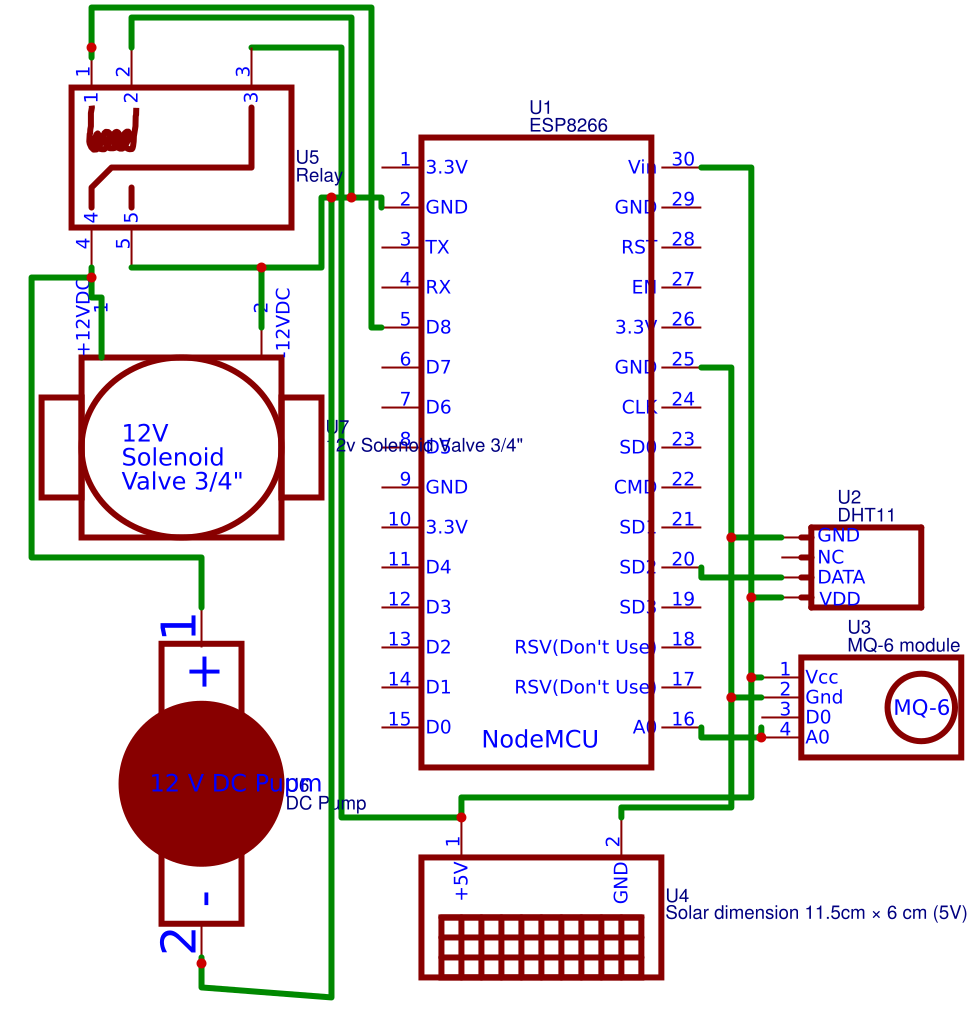
\includegraphics[width=5in]{35}
  \caption{Schematic Diagram of the System}\label{fig35}
\end{figure}
The gas sensor node is used for the monitoring and enhancing the kitchen safety of the home. The schematic and wiring diagram are presented in Figure 6.1. The DIO pin of MQ-2 is connected to the ESP8266 DIO pin 0. The other connections are same as temperature and humidity sensor node.\\

\section{Implementation of solar panel}
The ESP8266 is powered by the 3.7V battery that is connected to the Solar Lipo Charger in the battery input port. The solar cells are connected in the PWR In ports. The Vin and GND ports of the ESP8266 are connected to Vout ports of the Solar Lipo Charger.\\\\
The BME280 power is supplied by the 3.3V port in the ESP8266. The communication is done through the I2C lines (SDA / SCL). For the sleep mode, D0 need to be connected to reset pin (RST). To fix all components in the box, a preboard is used.
\begin{figure}[H]
  \centering
  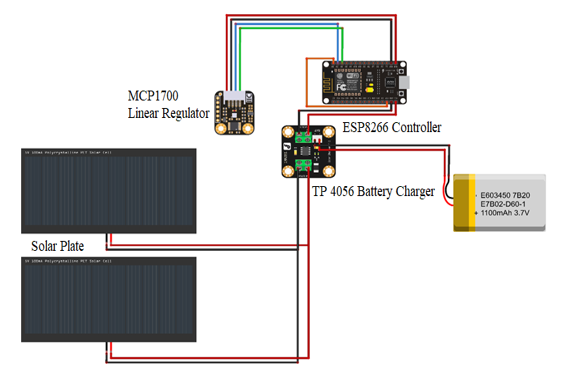
\includegraphics[width=6in]{36}
  \caption{Schematic diagram of a solar panel}\label{fig36}
\end{figure}
\section{Data Acquisition and Storage}
The software service running on the server performs the following two tasks:
\begin{enumerate}
  \item acquiring the data
  \item storing the data.
\end{enumerate}
A TCP socket receives sensor data created by the gateway in the form of TCP packets. Once a UDP packet is received, the sample data is extracted from the payload, and the source address of the ESP8266 Module that sent the data is extracted from the IPv6 source address of the TCP packet. The second task is to create a database for sensor sample extracted from the TCP packet using the information extracted from a TCP packet.\\
\begin{figure}[h]
  \centering
  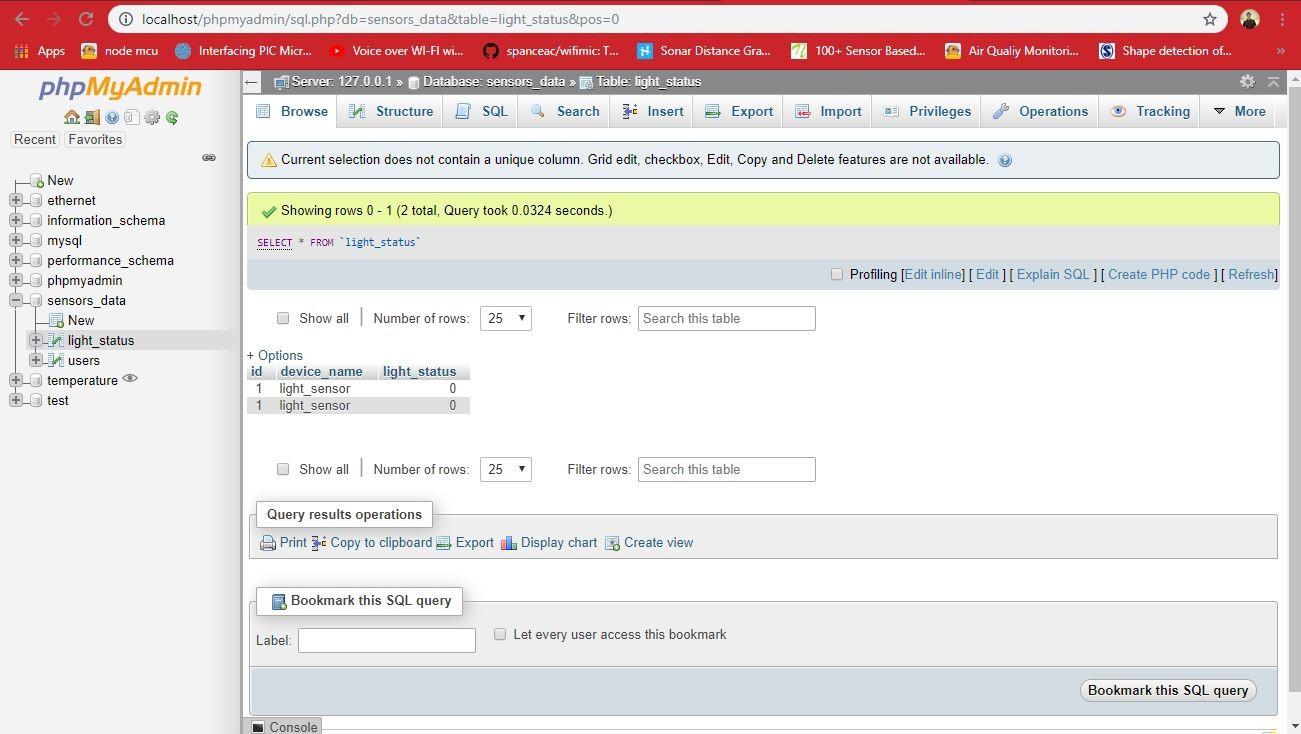
\includegraphics[width=6in]{39}
  \caption{Database Server (PHP my admin).}\label{fig39}
\end{figure}
\subsection{Database Server}
For hosting a website in the local machine XAMPP software package is used. Raspberry pi
works as a local server machine in which XAMPP package is installed. It facilitates in hosting website and works as a local database server. The software package also contains Apache MySQL server. The MySQL server is used to create database for the proposed system which is shown in Fig. 4.7. In MySQL server, data acquired by sensors are stored and retrieved when needed. Also, information’s of the end user are stored in the database. For the administration of the created database from remote panel PhpMyAdmin is also configured.
\begin{enumerate}
  \item Sensor ID
  \item Sensor Channel
  \item Date and time
  \item Sample Data
\end{enumerate}
When user sends a get request via the web interface PHP converts it into MySQL queries. PHP establishes the connection to the MySQL server and then fetch or post data according to the user command. The fetched data is then sent back to the html webpage for showing it to the user. HTML works in the client side for getting and PHP works in the server side for handling request for client. When the raspberry pi is powered and connected to the internet, the webpage hosted in it can be accessed from anywhere of the world. The sensor data from the TCP packet is stored in a MySQL database in an organized way. These sensors data are stored with a designated sensor ID, sensor channel and date and time in MySQL database so that the designed webpage can access those data.The data stored in the database can be viewed in the webpage.

\subsection{Receiving Data Samples}
The basic network communication between two programs is defined as socket. It is the endpoint of a two-way communication link. In an OS, the socket has two operating mode, client and server. When the OS acts as a client it is connected to the server to exchange data through the socket. In server mode the socket listens for incoming connections from clients. A socket is bound to a port number so that the TCP layer can identify the application that data is destined to be sent to. An endpoint is a combination of an IP address and a port number.\\
Data can be fetched from MySQL tables by executing SQL SELECT statement through PHP function mysql query.Several options are required to fetch data from MySQL.The most frequently used option is to use function mysql fetch array.
\begin{figure}[H]
  \centering
  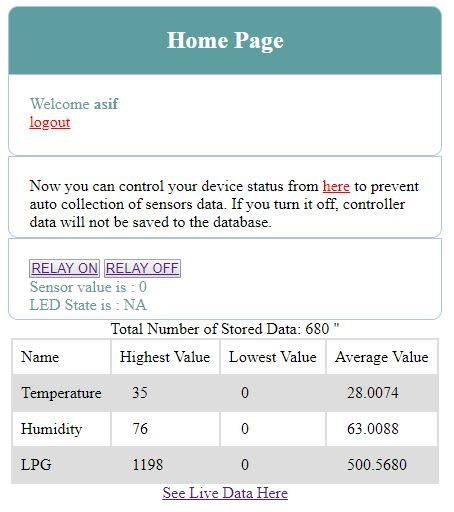
\includegraphics[width=4in]{38}
  \caption{Highest and lowest data samples. }\label{fig38}
\end{figure}



\section{ Web Interface}
The website in the server which is used to control the digital output pins is a group of pages
on World Wide Web containing buttons, sliders, sensors data and User Interface (UI) allowing the user to control the appliances all over the world through HTTP protocols. The webpage interface is used for controlling appliances, equipment like light, fan, cooler, air-conditioner etc. The status of different equipment is also visualized in the webpage. The developed webpage is presented in Figure-6.6.
\begin{figure}[H]
  \centering
  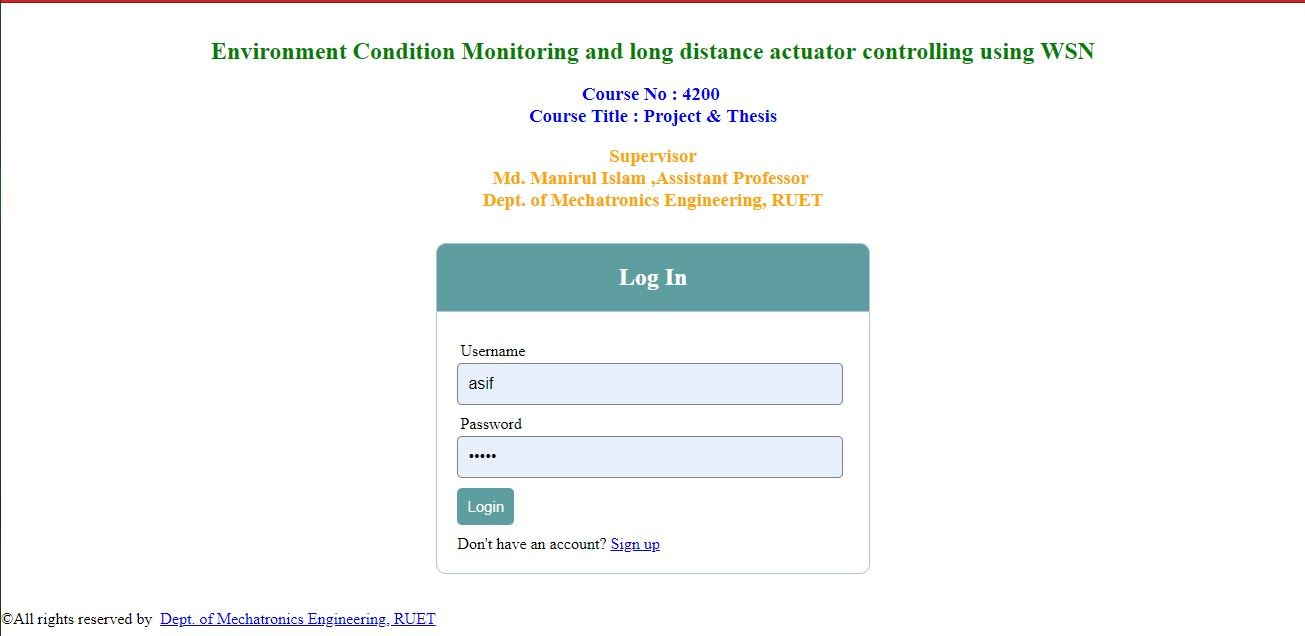
\includegraphics[width=6in]{40}
  \caption{Web interface}\label{fig40}
\end{figure}
Html files, .txt file and PHP files comprise the website to store data and to control the things by toggling the current state of the digital output pins. The web interface for the client side is implemented using HTML, CSS, JavaScript, Ajax, jQuery, and PHP script. The static web page is designed using HTML and CSS. CSS is a language that describes the style and elements of an HTML document. This static page is not interactive to user. To make it dynamic and interactive to the end user JavaScript is used for client-side scripting. jQuery is used to simplify the programing of JavaScript. It is a widely-used JavaScript library. Ajax is used as an interface language between client-side web applications and a server. It is a for user group of interrelated Web development techniques which is used on the client side to create asynchronous web applications. With Ajax, client-side web application can exchange data and status of the GPIO pin with a server asynchronously in the background without interfering with the display and behavior of the existing page. To continuously extract data from the MySQL data base A PHP script is written.
\section{Retrieving Data from Database}
To retrieve data from database the sensor id, sensor channel, and data and time range are required. These parameters are used to create a SQL query to the database to retrieve the required sensor samples. A PHP script is written which contains those database parameters to generate a SQL query for the purpose of retrieving data. These data are placed on JSON array. The output of the JSON array are then transferred to the web browser. The web browser calls the PHP scripts to retrieve data by running a java script. For the control of GPIO pins another PHP script which toggles the current state of the GPIO pins is also called by the web page to generate a control message when graphical interface buttons, sliders are operated.Although records are normally retrieved in the order in which they are inserted into the database, data cannot rely on a particular order being preserved. If created database was backed up and restored, or if a maintenance operation was performed on the database, MySQL might alter the order in which records were stored internally.
\begin{figure}[H]
  \centering
  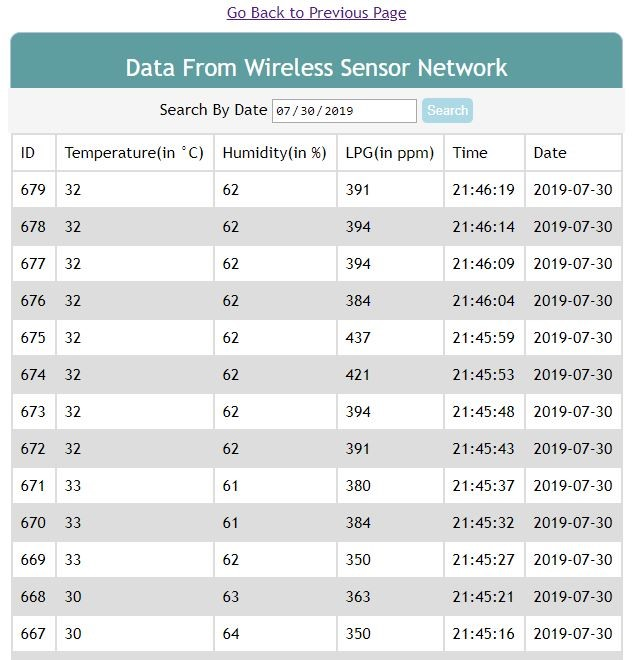
\includegraphics[width=4in]{37}
  \caption{Data stored in database.}\label{fig37}
\end{figure}
\section{Controlling actuator from the web server}
To take you one step ahead towards WSN development, today we will make our own web server to host a webpage and control any appliance remotely from anywhere in the world. Here ESP12E NodeMCU was used as webserver, although any ESP module can be used here.\\\\
In simple terms, Web server is a place where we can store the web pages, process them and deliver them to the web clients. A protocol is used to establish and transfer information between web client and server. This protocol is known as Hypertext Transfer Protocol (HTTP). In this protocol, communication is initiated by making a request for a particular web page using HTTP GET request and the server responds with the content of that web page. If server does not respond it will through an error message i.e. 404 Error. Webpages delivered by the server are mostly in HTML coding.
\begin{figure}[H]
  \centering
  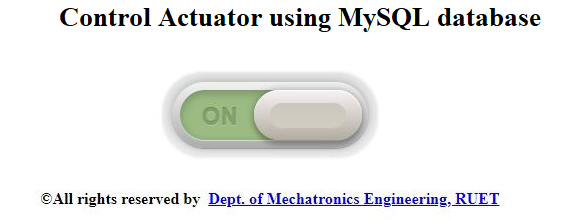
\includegraphics[width=6in]{42}
  \caption{Controlling Actuator from server }\label{fig42}
\end{figure}
All the websites are hosted on some webserver, mostly Linux based operating system is used on webservers. Any computer can be converted into a webserver, provided that it is connected to the network. We have previously done many webserver projects with different microcontrollers. Raspberry pi already has inbuilt Wi-Fi module so it doesn't need any other hardware to turn it into a webserver, whereas other microcontroller needs some network connecter (ESP module) for a webserver.
\section{Final Setup}
Final setup of the project was made by the components described earlier.The setup outlook was made by using PVC board and all the components were calibrated before installation.The system performance was satisfactory.
\begin{figure}[H]
  \centering
  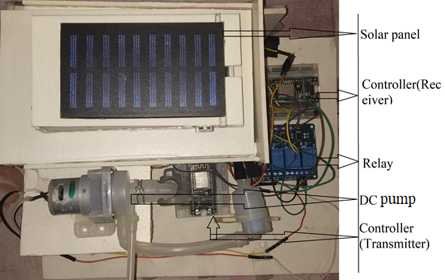
\includegraphics[width=4in]{44}
  \caption{Implemented system  }\label{fig44}
\end{figure}
The relay was also did the satisfactory level performance.The system was under a trial about 1 hour randomly.In trial period the relay control state wasn't show any error.The Figure 6.9 represent the relay state with respect to time.
\begin{figure}[h]
  \centering
  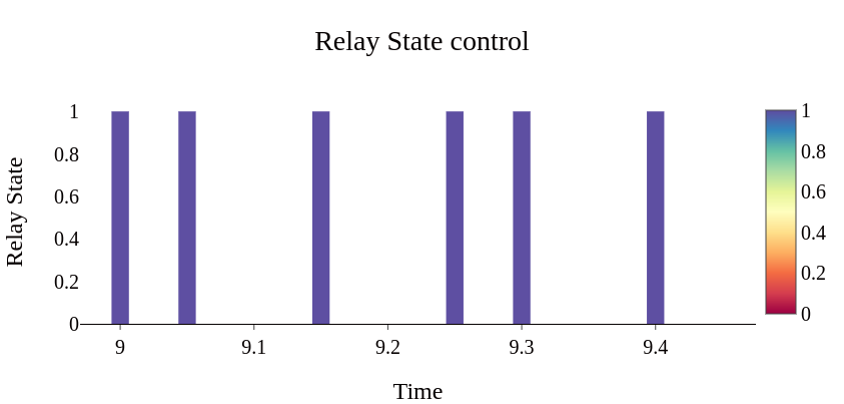
\includegraphics[width=4 in]{47}
  \caption{Relay state ON/OFF using Feedforward \& Feedback control system (For Actuator Controlling}\label{fig46}
\end{figure}

\section{Chapter Summery}
In this Chapter the experimental setup is described along with the database which was created for the WSN sensor node.This chapter in this volume have presented the best available knowledge of database and some of technologies and tools available for this setup.The objectives of the chapter is to apply this knowledge in the development of the WSN node and the database for storing the data alongside for controlling the Actuator.  
\chapter{\textbf{Test Results \& Discussions}}
\begin{justify}
From experimental data, various calculations were performed using ‘MATLAB’ environment. The Digital Signal Analysis- Toolbar is a great tool for signal processing and smoothing. As the data were some arbitrary thus a processing is needed to overcome the problem. Mainly Fast Fourier Transformations were performed for better signal processing. The below figures are the results:
\end{justify}
\section{Sensor Signal Analysis \& Processing}

From experimental data, various calculations were performed using ‘MATLAB’ environment. The Digital Signal Analysis- Toolbar is a great tool for signal processing and smoothing. As the data were some arbitrary thus a processing is needed to overcome the problem. Mainly Fast Fourier Transformations were performed for better signal processing. The below figures are the results:
\begin{enumerate}[label=\roman*]
\setlength{\parskip}{0.0pt}
\item \textbf{Coherence Estimation via Welch Method:}In digital signal processing, coherence is a statistics between two functions or
signals which is used to estimate the power transfer of the input and output in a linear/linear time-invariant system. This algorithm is based on standard MATLAB’s tools. The standard derivation of the mean is computed as \cite{sethi2017internet,tsang2017iot,zawawi2018electromyography,gres2019orthogonal,regalia2018adaptive,de2013inverse,cohen2018automated,van2018signal,anchal2018nonlinearity,seichter2018online,lewicki2009eddy,hijazi2018ambient};\par


\begin{equation}\tag{7.1}
 \sigma  ( f ) = \sqrt[]{\frac{2}{N \vert  \Upsilon  ( f ) ^{2} \vert } ( 1- \vert  \Upsilon  ( f )  \vert ^{2} ) ^{2}}
\end{equation}
\begin{justify}
Where,
\end{justify}


\begin{equation}\tag{7.2}
 \vert  \Upsilon  ( f )  \vert ^{2}= \frac{ \vert P_{xy} ( f )  \vert ^{2}}{P_{xx} ( f ) .P_{yy} ( f ) }
\end{equation}
\begin{justify}
Is the coherence function.In signal processing, the coherence is a statistic that can be used to examine the relation between two signals or data sets. It is commonly used to estimate the power transfer between input and output of a linear system. If the signals are ergodic, and the system function linear, it can be used to estimate the causality between the input and output.The computed coherence (Figure 7.1) indicates that at most of the major ocean tidal frequencies the variation of groundwater level at this particular site is over 90\% due to the forcing of the ocean tides. However, one must exercise caution in attributing causality. If the relation (transfer function) between the input and output is nonlinear, then values of the coherence can be erroneous. Another common mistake is to assume a causal input/output relation between observed variables, when in fact the causative mechanism is not in the system model. By using equations-(7.1) $\&$  (7.2), Figure-7.1, can be plotted. Here, Figure-7.1 depicts the coherence estimation via Welch method. This figure shows that no data has been overlapped into one another.
\end{justify}

\begin{figure}[H]
	\begin{Center}
		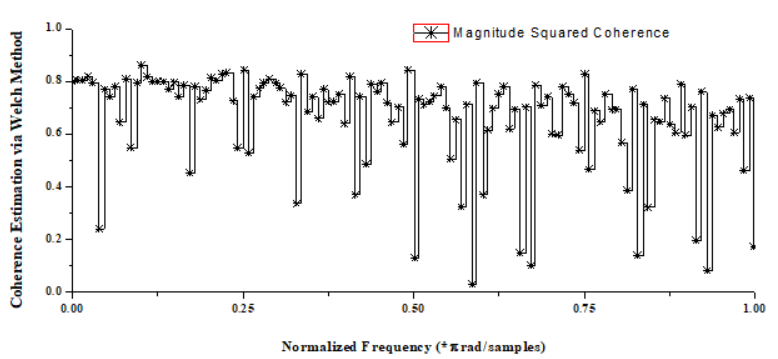
\includegraphics[width=6in,height=2in]{15}
		\caption{ Coherence estimation via Welch method }
		\label{fig:_1_Coherence_estimation_via_Welch_method_}
	\end{Center}
\end{figure}


%%%%%%%%%%%%%%%%%%%% Figure/Image No: 24 Ends here %%%%%%%%%%%%%%%%%%%%

\par

\setlength{\parskip}{8.04pt}
\par

\setlength{\parskip}{0.0pt}
The Figure 7.2, denotes the magnitude response curve. The rms signal-to-noise ratio for an ideal N-bit converter is:\par


\begin{equation}\tag{7.3}
Signal to Noise Ratio (SNR) = 20log_{10}\frac{r.m.s value of F_{s} input}{r.m.s value of quantization noise}
\end{equation}

\begin{equation}\tag{7.4}
or, SNR = 20log_{10}\frac{q^{2^{N}}/2\sqrt[]{2}}{q/\sqrt[]{2}}=20log_{10}2^{N}+20log_{10}\sqrt[]{\frac{3}{2}}
\end{equation}
\begin{justify}
SNR = 6.02N + 1.76 dB (13), over the Nyquist bandwidth of interest.
\end{justify}\par



%%%%%%%%%%%%%%%%%%%% Figure/Image No: 25 starts here %%%%%%%%%%%%%%%%%%%%

\begin{figure}[H]
	\begin{Center}
		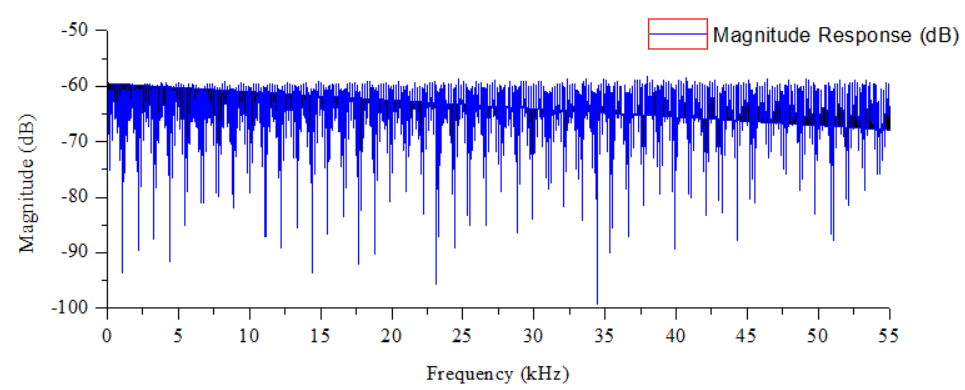
\includegraphics[width=5.91in,height=2.16in]{16}
		\caption{ Magnitude Response Graph (Gas Sensor)}
		\label{fig:_2_Magnitude_Response_Graph_Gas_Sensor}
	\end{Center}
\end{figure}
 The transfer function is independent of the spectral properties of the stimulus as long as the system behaves linearly and as long as the input and output signals are measured at sufficient SNR.

%%%%%%%%%%%%%%%%%%%% Figure/Image No: 25 Ends here %%%%%%%%%%%%%%%%%%%%

\par

\par

\begin{justify}
Figure 7.3, represents the combination of magnitude and phase response. The plot shows limited errors.
\end{justify}\par



%%%%%%%%%%%%%%%%%%%% Figure/Image No: 26 starts here %%%%%%%%%%%%%%%%%%%%

\begin{figure}[H]
	\begin{Center}
		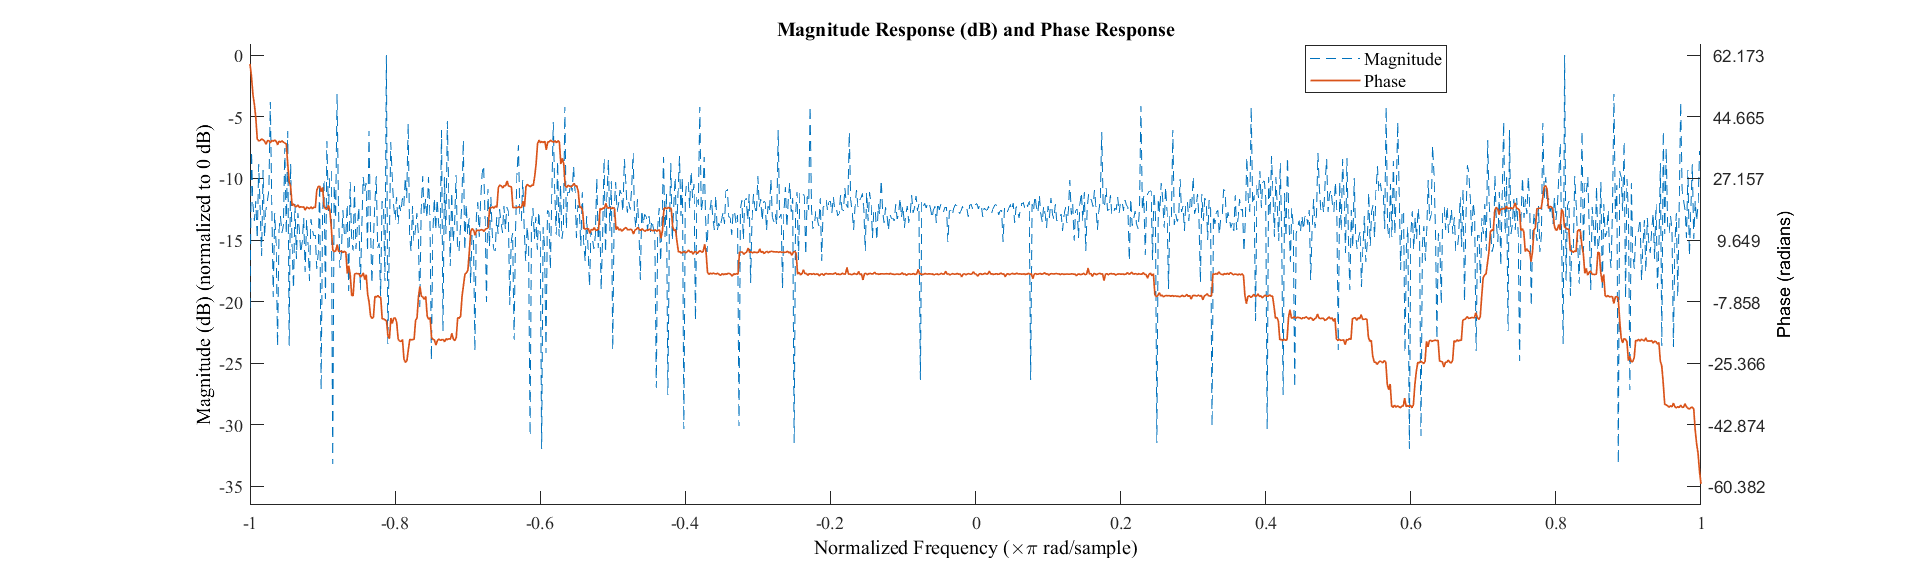
\includegraphics[width=5.52in,height=2.73in]{17}
		\caption{ Magnitude and Phase Response (Gas Sensor) }
		\label{fig:_3_Magnitude_and_Phase_Response_Gas_Sensor_}
	\end{Center}
\end{figure}


%%%%%%%%%%%%%%%%%%%% Figure/Image No: 26 Ends here %%%%%%%%%%%%%%%%%%%%

\par

\par

\item \textbf{Time Domain signal processing:} Now, using the gas sensor data Time-domain graph was plotted in Figure-7.4 to Figure-7.7,
along with a 3rd and 8\textsuperscript{th} order Fast Fourier Transformation (FFT) of the signal for better analysis. The Fourier series is a sum of sine and cosine functions that describes a periodic signal. It is represented in either the trigonometric form or the exponential form. The toolbox provides this trigonometric Fourier series form [45]:\par


\begin{equation}\tag{7.5}
y=a_{0}+ \sum _{i=1}^{n}a_{i}cos ( iwx ) +b_{i}sin ( iwx )
\end{equation}
\setlength{\parskip}{8.04pt}
where a\textsubscript{0} models a constant (intercept) term in the data and is associated with the i = 0 cosine term, w is the fundamental frequency of the signal, n is the number of terms (harmonics) in the series, and 1 $ \leq $  n $ \leq $  8.Time domain refers to the analysis of mathematical functions, physical signals or time series of economic or environmental data, with respect to time. In the time domain, the signal or function's value is known for all real numbers, for the case of continuous time, or at various separate instants in the case of discrete time. An oscilloscope is a tool commonly used to visualize real-world signals in the time domain. A time-domain graph shows how a signal changes with time, whereas a frequency-domain graph shows how much of the signal lies within each given frequency band over a range of frequencies. A Savitzky–Golay filter is a digital filter that can be applied to a set of digital data points for the purpose of smoothing the data, that is, to increase the signal-to-noise ratio without greatly distorting the signal. This is achieved, in a process known as convolution, by fitting successive sub-sets of adjacent data points with a low-degree polynomial by the method of linear least squares. Figure-7.4 depicts the plots of Raw analog, Savitzky Golay Filtered value, moving avg. filtered value and the median plot.\par



%%%%%%%%%%%%%%%%%%%% Figure/Image No: 27 starts here %%%%%%%%%%%%%%%%%%%%

\begin{figure}[H]
	\begin{Center}
		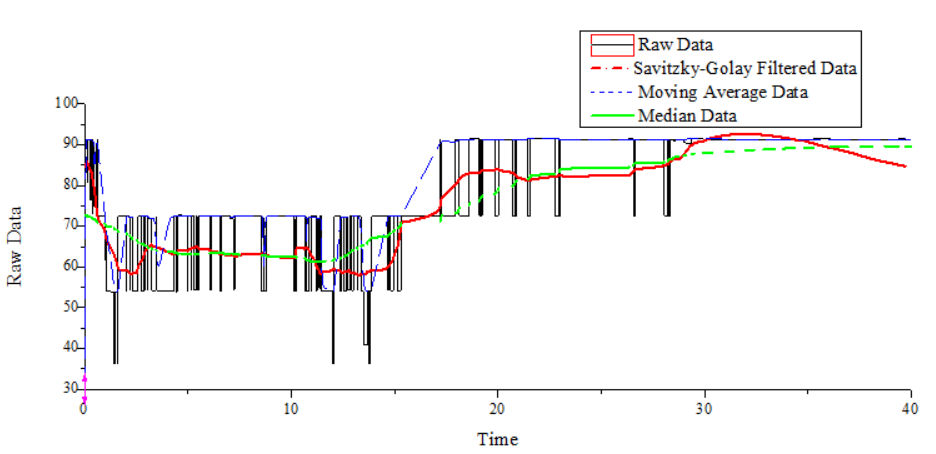
\includegraphics[width=6.5in,height=2.72in]{18}
		\caption{Processed Signal (PPM vs Time)}
		\label{fig:_4_Processed_Signal_PPM_vs_Time}
	\end{Center}
\end{figure}


%%%%%%%%%%%%%%%%%%%% Figure/Image No: 27 Ends here %%%%%%%%%%%%%%%%%%%%

\setlength{\parskip}{0.0pt}
\par

\par


\vspace{\baselineskip}

\vspace{\baselineskip}

\vspace{\baselineskip}
\begin{justify}
Figure 7.5 shows the Furrier fitted curve for gas sensor value.
\end{justify}\par



%%%%%%%%%%%%%%%%%%%% Figure/Image No: 28 starts here %%%%%%%%%%%%%%%%%%%%

\begin{figure}[H]
  \centering
  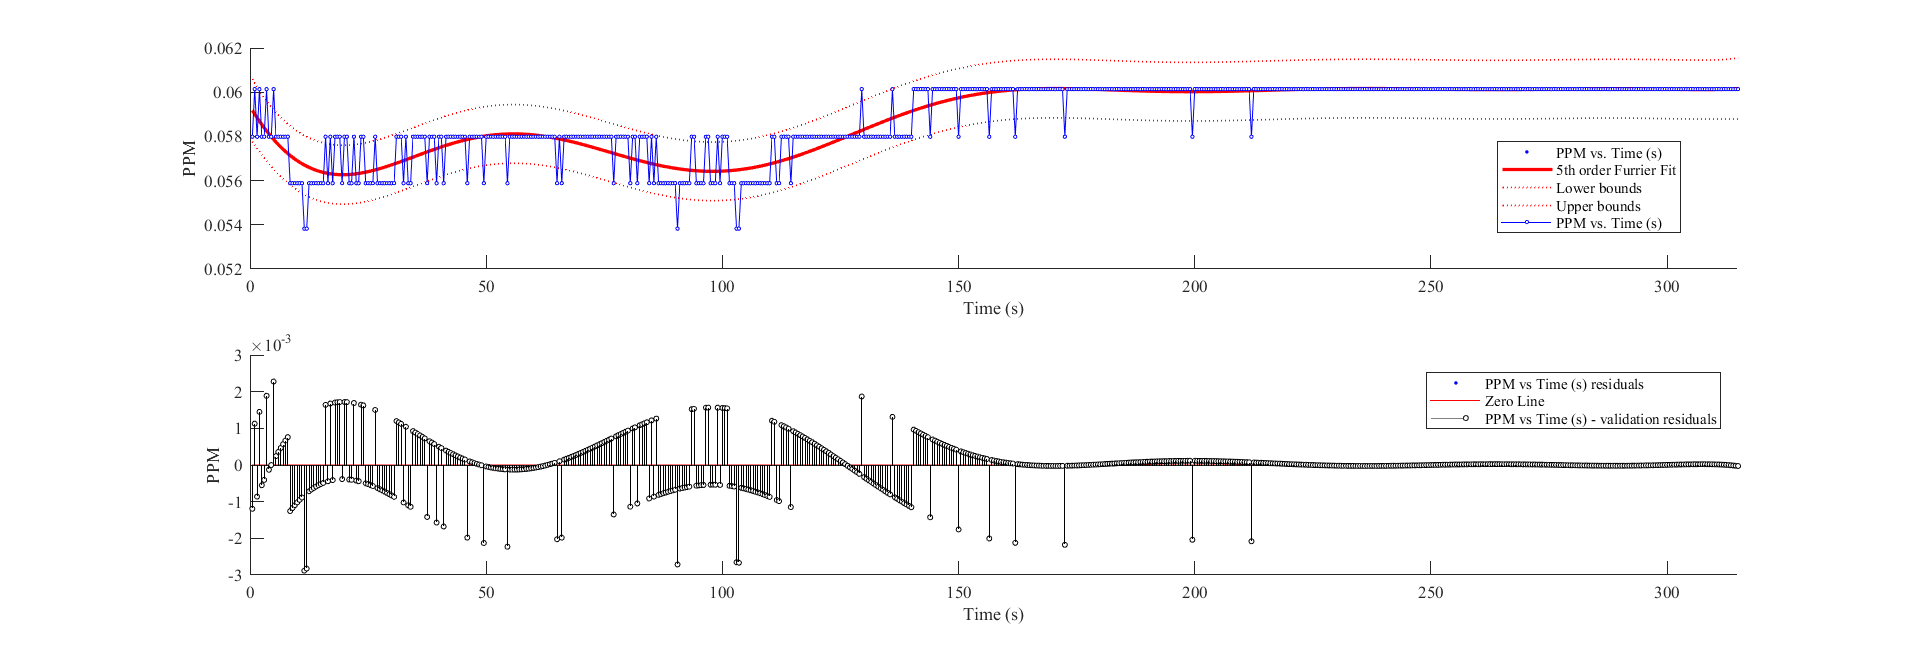
\includegraphics[width=6.5in,height=2.38in]{19}
  \caption{Furrier fitted curve for gas sensor value}\label{fig19}
\end{figure}
%\begin{figure}[H]
%	\begin{Center}
%		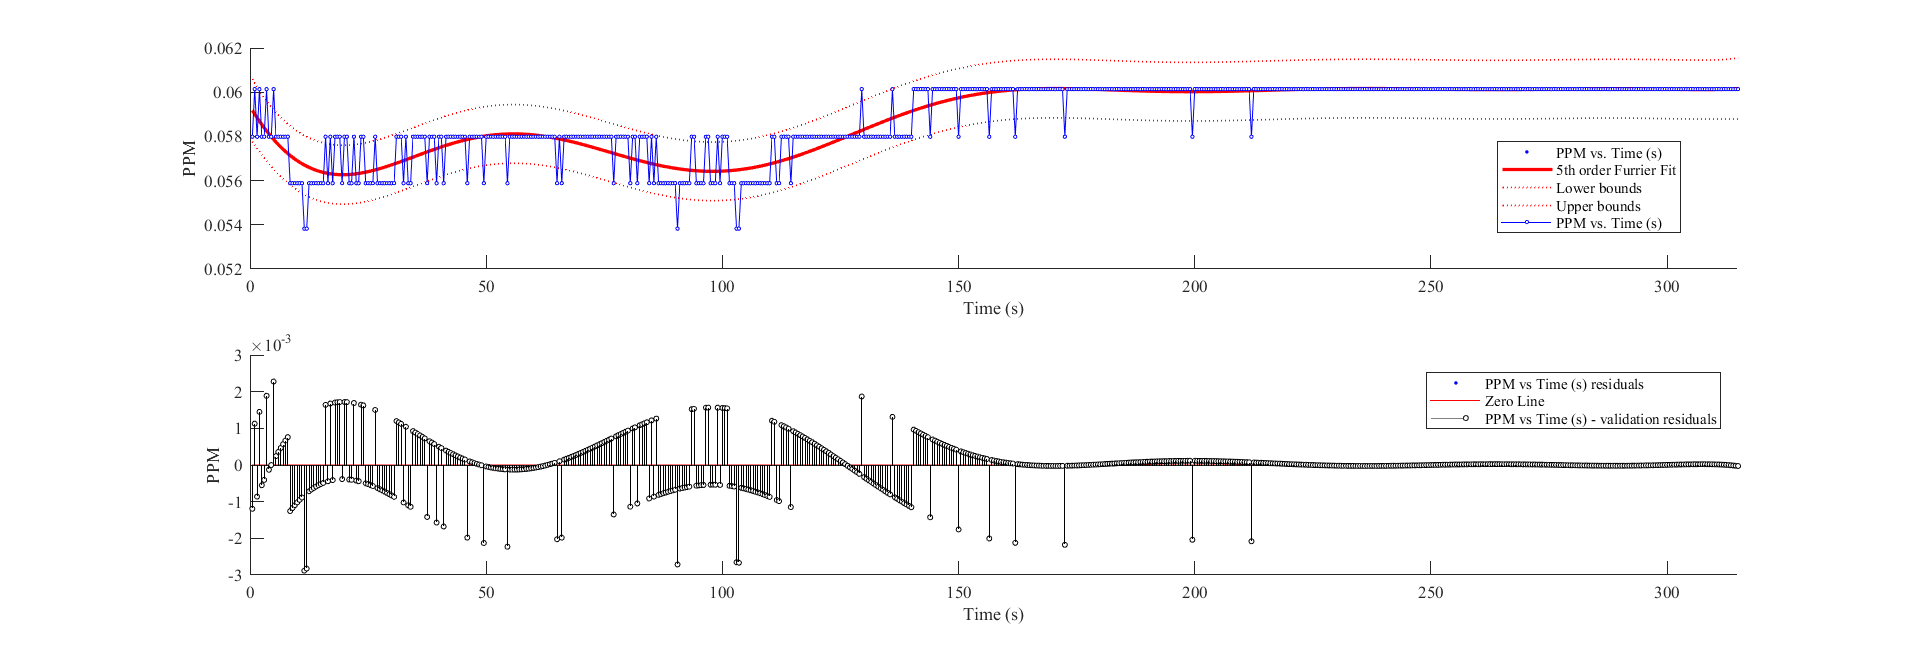
\includegraphics[width=6.5in,height=2.38in]{19}
%	\end{Center}
%\end{figure}


%%%%%%%%%%%%%%%%%%%% Figure/Image No: 28 Ends here %%%%%%%%%%%%%%%%%%%%

\par

\par


\vspace{\baselineskip}
\begin{justify}
The below Figure 7.6 $\&$  7.7 are the same plots as Figure 7.4 $\&$  7.5, but those value represents the Temperature and Humidity.
\end{justify}\par



%%%%%%%%%%%%%%%%%%%% Figure/Image No: 29 starts here %%%%%%%%%%%%%%%%%%%%

\begin{figure}[H]
	\begin{Center}
		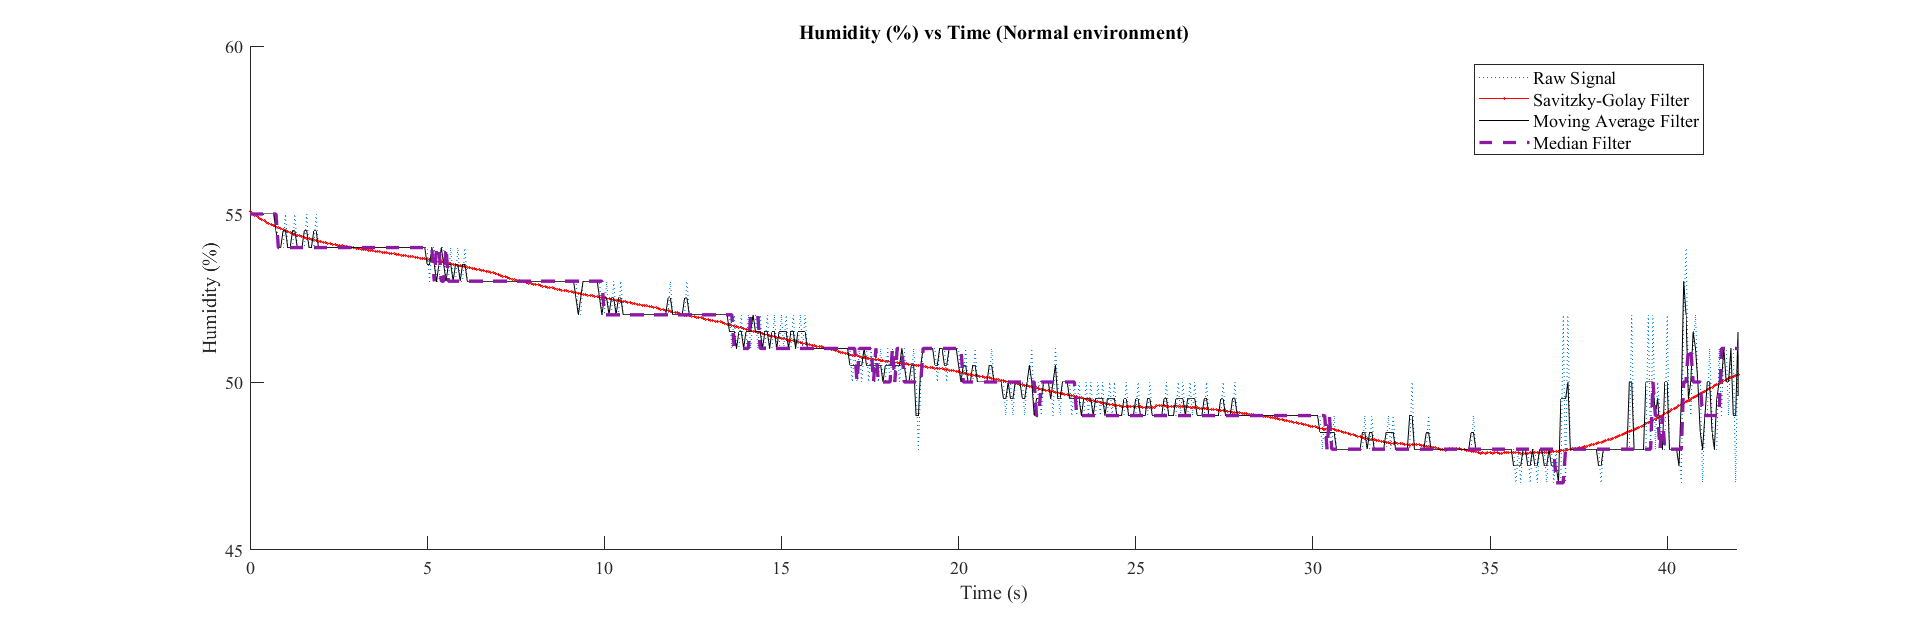
\includegraphics[width=6.36in,height=2.81in]{20}
		\caption{Processed Signal (Humidity vs Time)}
		\label{fig:_6_Processed_Signal_Humidity_vs_Time}
	\end{Center}
\end{figure}


%%%%%%%%%%%%%%%%%%%% Figure/Image No: 29 Ends here %%%%%%%%%%%%%%%%%%%%

\par

\par


\vspace{\baselineskip}


%%%%%%%%%%%%%%%%%%%% Figure/Image No: 30 starts here %%%%%%%%%%%%%%%%%%%%

\begin{figure}[H]
	\begin{Center}
		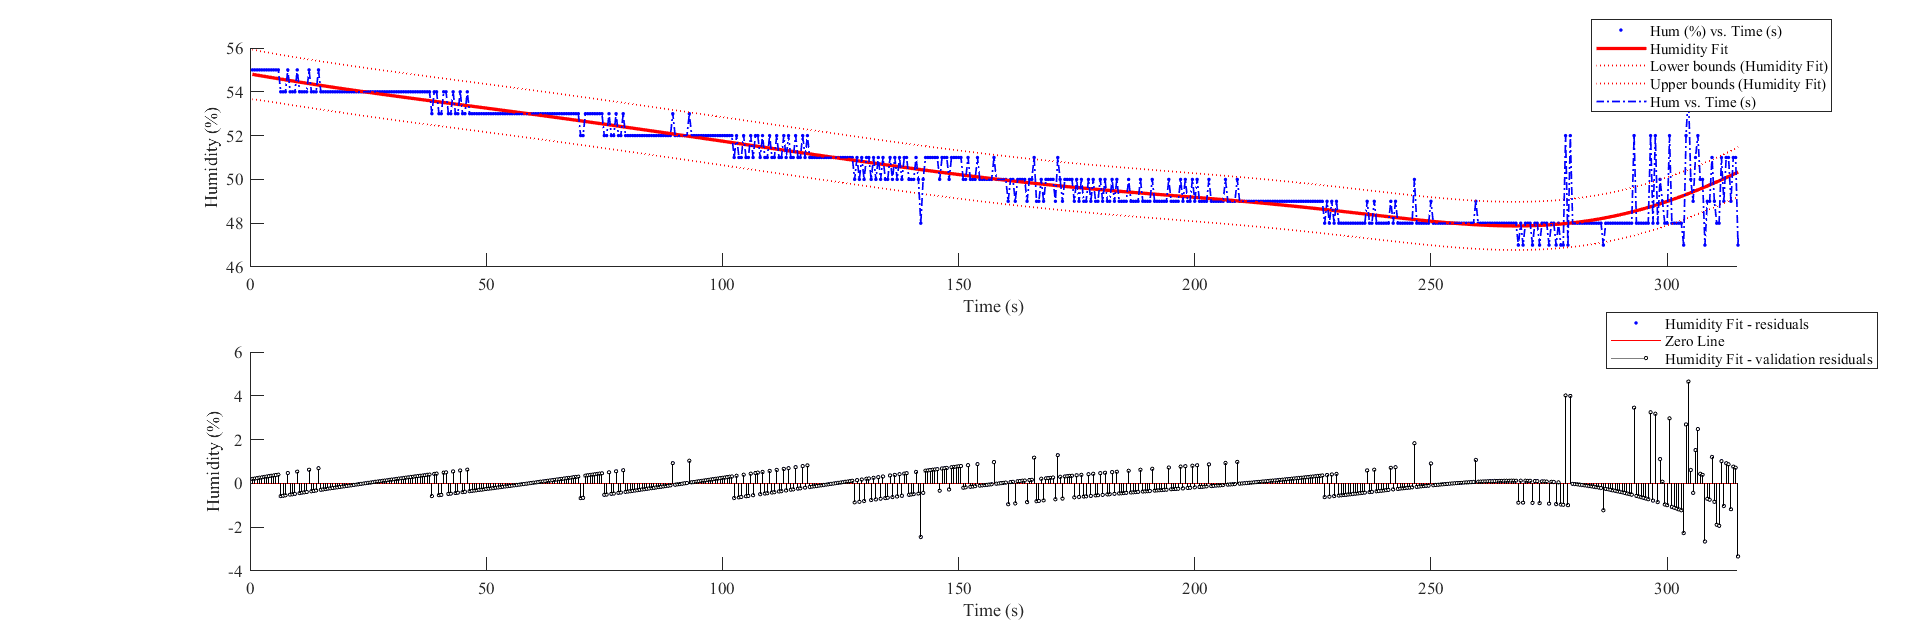
\includegraphics[width=6.25in,height=3.47in]{21}
	\end{Center}
\caption{Humidity vs Time domain graph with $8^{th}$ order furrier transform using 95\% of confidence limit}
\end{figure}


%%%%%%%%%%%%%%%%%%%% Figure/Image No: 30 Ends here %%%%%%%%%%%%%%%%%%%%

\par

\par

\begin{justify}
It shows that an 8\textsuperscript{th} order Fourier Transformation will result in a better signal conditioning.
\end{justify}\par

\item \textbf{Group delay response analysis:} In signal processing, group delay is the time delay of the amplitude envelopes of the various
sinusoidal components of a signal through a device under test, and is a function of frequency for each component. Phase delay, in contrast, is the time delay of the phase as opposed to the time delay of the amplitude envelope. Now from convolution theorem [46-50],\par


\begin{equation}\tag{7.6}
If, y(t) = ( h\ast x)(t) \cong \int _{-inf.}^{+inf.}x(u)h(t-u)du
\end{equation}
\begin{justify}
In frequency domain; Y(s) = H(s).X(s). Then, on simplification and using some computational techniques it can be showed that;
\end{justify}\par


\begin{equation}\tag{7.7}
x(t) =a(t) cos(\omega t+ \theta)
\end{equation}
\begin{justify}
 $\&$  By assuming,  \(  \vert \frac{dlog(a(t))}{dt} \vert  \ll  \omega  \) , the output of such an LTI (Linear time-invariant) system can be approximated as,
\end{justify}\par


\begin{equation}\tag{7.8}
y(t)=|H(i\omega)|a(t-\tau_g)cos(\omega(t-\tau_{\phi})+\theta)
\end{equation}
\begin{justify}
$\&$  they can be computed from the phase shift  \(  \phi  \)  $ \{ $ $\textbackslash$ displaystyle $\textbackslash$ displaystyle $\textbackslash$ phi $ \} $  by,  \(  \tau_{g} (  \omega  ) =-\frac{d \phi  (  \omega  ) }{d \omega } \)  and  \(  \tau_{ \phi } (  \omega  ) =-\frac{ \phi  (  \omega  ) }{ \omega } \) . From equation-(16), it can be shown that the group delay, $ \{ $ $\textbackslash$ displaystyle $\textbackslash$ displaystyle $\textbackslash$ tau \_$ \{ $ g$ \} $ $ \} $  \(  \tau_{g} \) , and phase delay, $ \{ $ $\textbackslash$ displaystyle $\textbackslash$ displaystyle $\textbackslash$ tau \_$ \{ $ $\textbackslash$ phi $ \} $ $ \} $  \(  \tau_{ \phi } \) , are frequency-dependent. To understand the convolution process of the LTI system, let the notation $ \{ $  \( x ( u- \tau ) ;u \) $ \} $  represent the function  \( x ( u- \tau )  \)  with variable \(  u and \)  constant  \(  \tau. \)  Then a continuous-time system transforms an input function (x) into an output function (y) and in general, every value of the output can depend on every value of the input. This concept is represented by;
\end{justify}\par


\begin{equation}\tag{7.9}
y ( t ) \cong O_{t} ( x )
\end{equation}
\begin{justify}
Where, \textit{O\textsubscript{t }}is the transformation operator for time (t). In a typical system, y(t) depends most heavily on the values of x that occurred near the time t. So, for a linear system;
\end{justify}\par


\begin{equation}\tag{7.10}
O_t\{\int_{-inf}^{+inf}c_{\tau}.x_{\tau}(u)d\tau;u\}=\int_{-inf}^{+inf}c_{\tau}.y_{\tau}(u)d\tau;u
\end{equation}
\begin{justify}
$\&$  the time-invariance requirement is;
\end{justify}\par


\begin{equation}\tag{7.11}
O_t\{x(u-\tau);u\}=y(t-\tau)\cong O_{t-\tau}\{x\}
\end{equation}
\begin{justify}
From, eqn-10, the impulse response can be noted as;
\end{justify}\par


\begin{equation}\tag{7.12}
h ( t ) \cong O_{t} \{  \delta u; u \}
\end{equation}
\begin{justify}
From, equations-(7.10) to (7.12), using Amplitude vs samples; Figure 7.8 to Figure 7.10, can be drawn. Figure 7.8 is the group delay response plot for gas sensor which shows that between 11.3-12.2 kHz of sampling frequency the delay remains constant.
\end{justify}\par



%%%%%%%%%%%%%%%%%%%% Figure/Image No: 31 starts here %%%%%%%%%%%%%%%%%%%%

\begin{figure}[H]
	\begin{Center}
		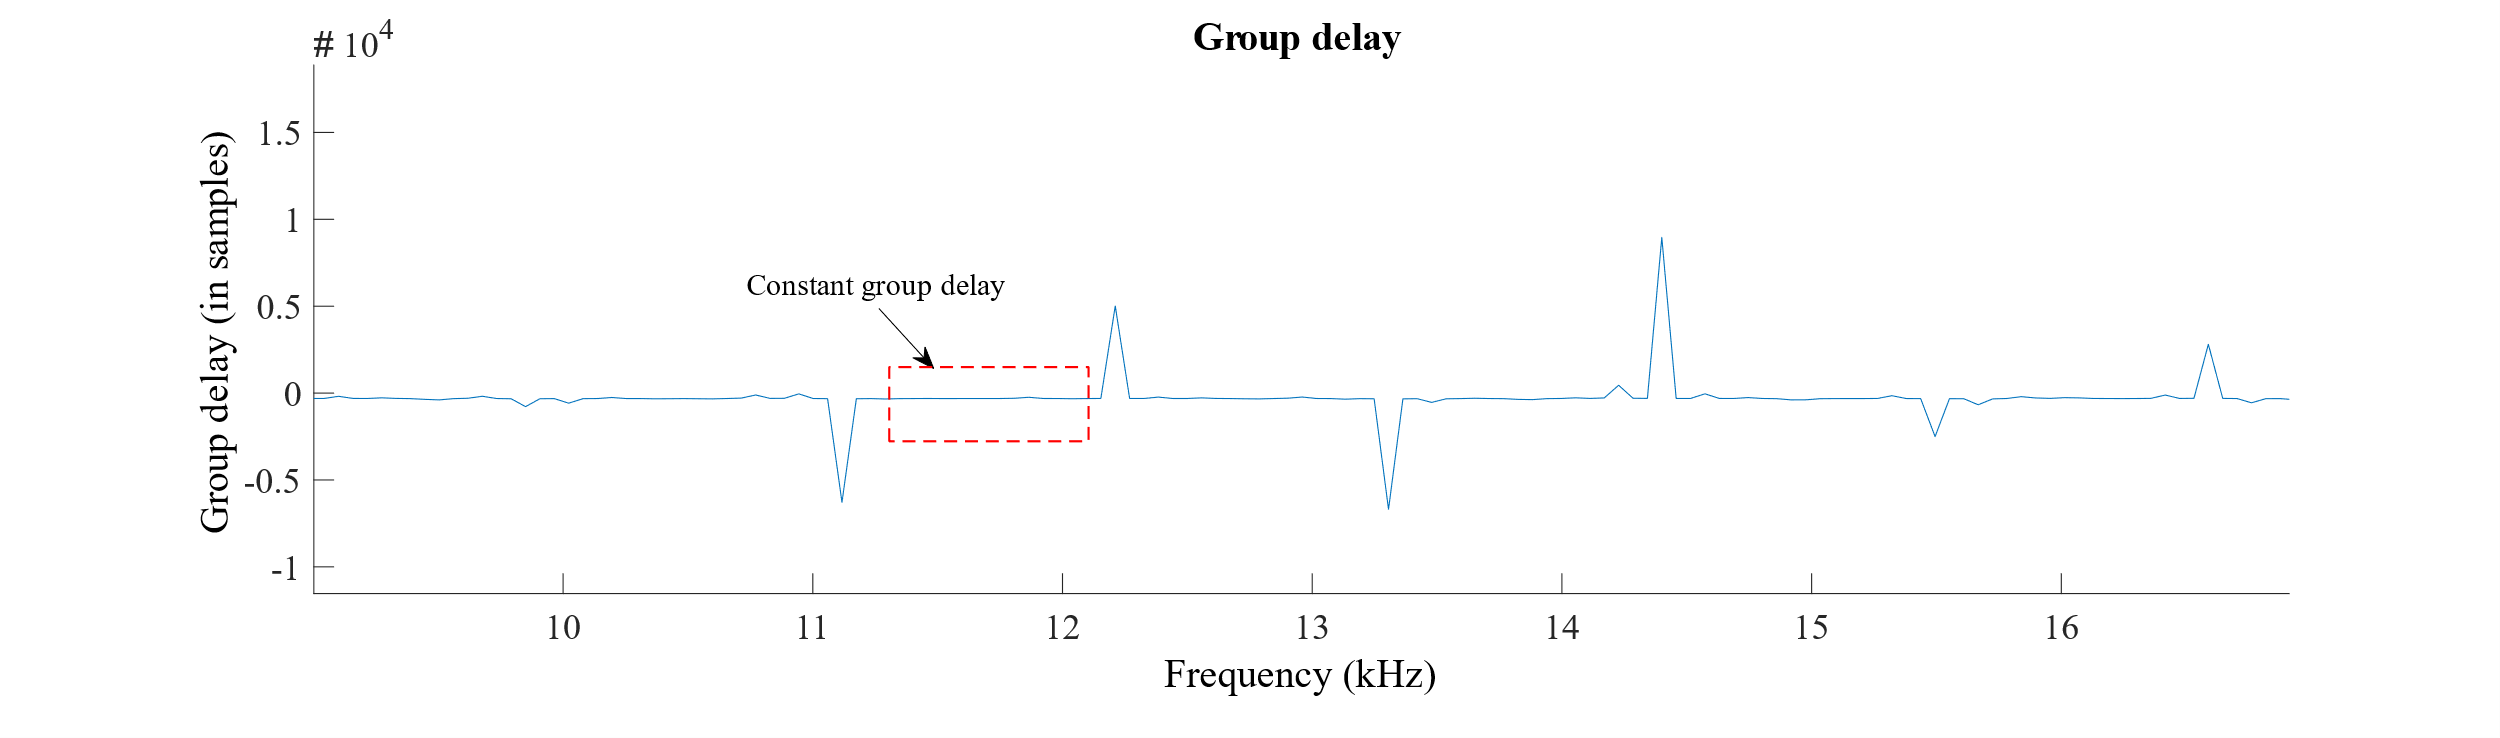
\includegraphics[width=6.44in,height=2.42in]{22}
		\caption{Group delay response}
		\label{fig:_8_Group_delay_response}
	\end{Center}
\end{figure}


%%%%%%%%%%%%%%%%%%%% Figure/Image No: 31 Ends here %%%%%%%%%%%%%%%%%%%%

\par

\par

\begin{justify}
Figure 7.9 represents the phase delay (with respect to samples), it shows also that 11.3-12.2 kHz sampling is the most effective one for the controller.
\end{justify}\par



%%%%%%%%%%%%%%%%%%%% Figure/Image No: 32 starts here %%%%%%%%%%%%%%%%%%%%

\begin{figure}[H]
	\begin{Center}
		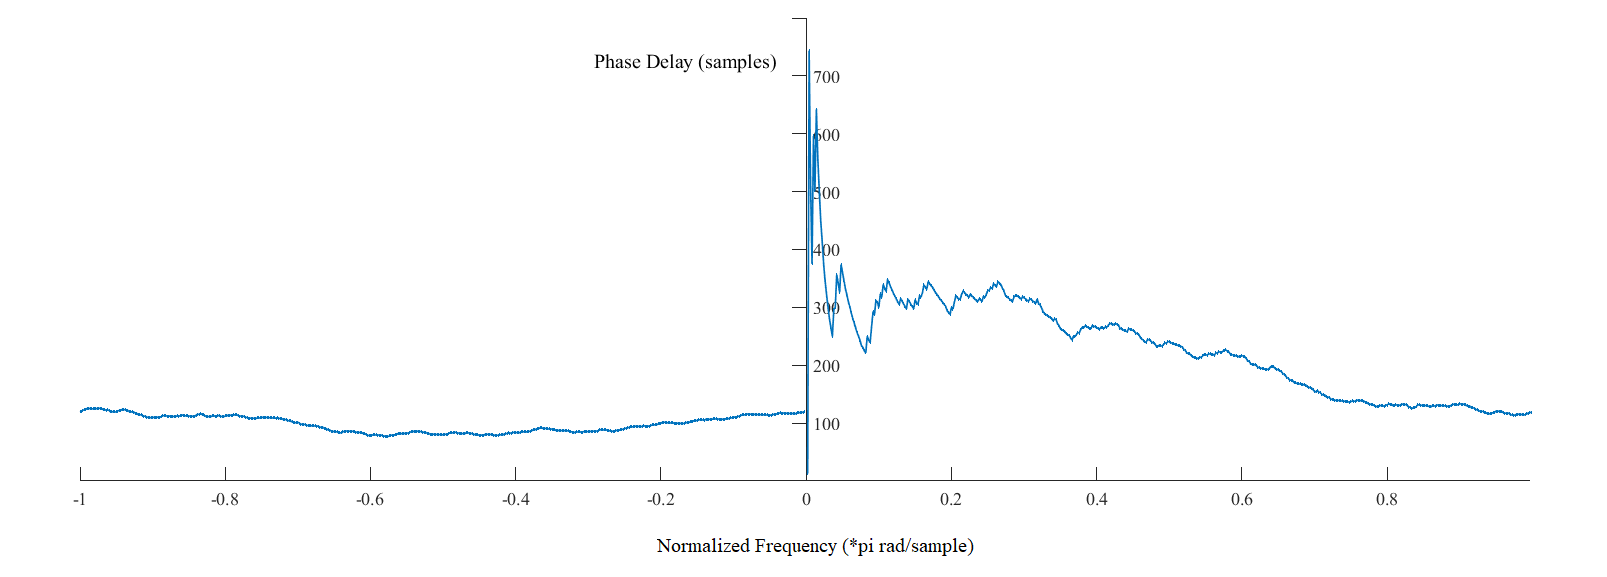
\includegraphics[width=6.5in,height=2.67in]{23}
		\caption{Phase Delay Samples}
		\label{fig:_9_Phase_Delay_Samples}
	\end{Center}
\end{figure}


%%%%%%%%%%%%%%%%%%%% Figure/Image No: 32 Ends here %%%%%%%%%%%%%%%%%%%%

\par

\par


\vspace{\baselineskip}
\begin{justify}
A pole-zero plot shows the location in the complex plane of the poles and zeros of the transfer function of a dynamic system, such as a controller, compensator, sensor, equalizer, filter, or communications channel. ... For a CT system, the plane in which the poles and zeros appear is the s plane of the Laplace transform.
\end{justify}\par



%%%%%%%%%%%%%%%%%%%% Figure/Image No: 33 starts here %%%%%%%%%%%%%%%%%%%%

\begin{figure}[H]
	\begin{Center}
		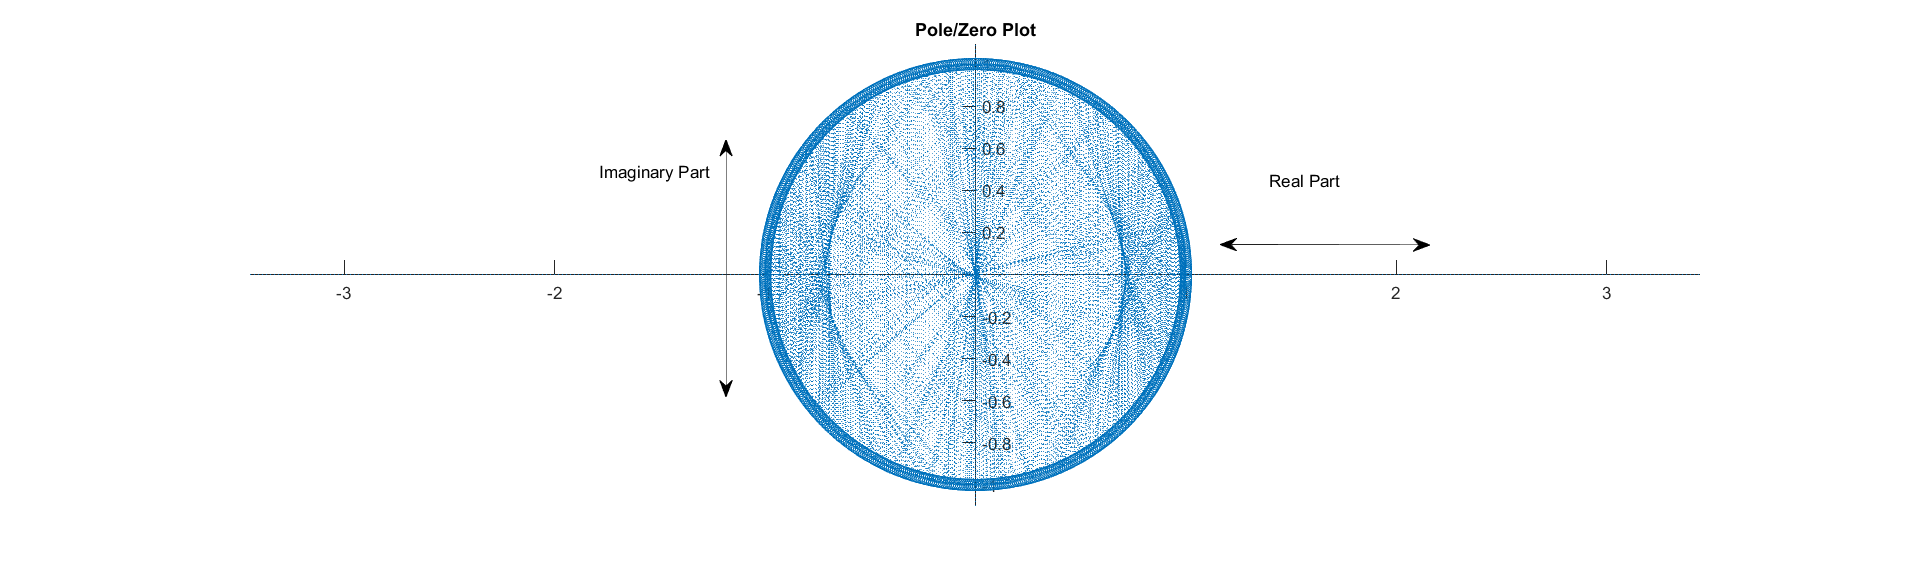
\includegraphics[width=6.55in,height=2.29in]{24}
	\end{Center}
\caption{Pole Zero Plot.}
\end{figure}
Figure 7.10, denotes the pole zero plot for the system, which shows that this system has some noise but ultimately it is stable. Figure 7.11 is the round-off noise power spectrum plot for the system. It shows some unnatural noise in the system.

%%%%%%%%%%%%%%%%%%%% Figure/Image No: 33 Ends here %%%%%%%%%%%%%%%%%%%%

\par

\par


\vspace{\baselineskip}


%%%%%%%%%%%%%%%%%%%% Figure/Image No: 34 starts here %%%%%%%%%%%%%%%%%%%%

\begin{figure}[H]
	\begin{Center}
		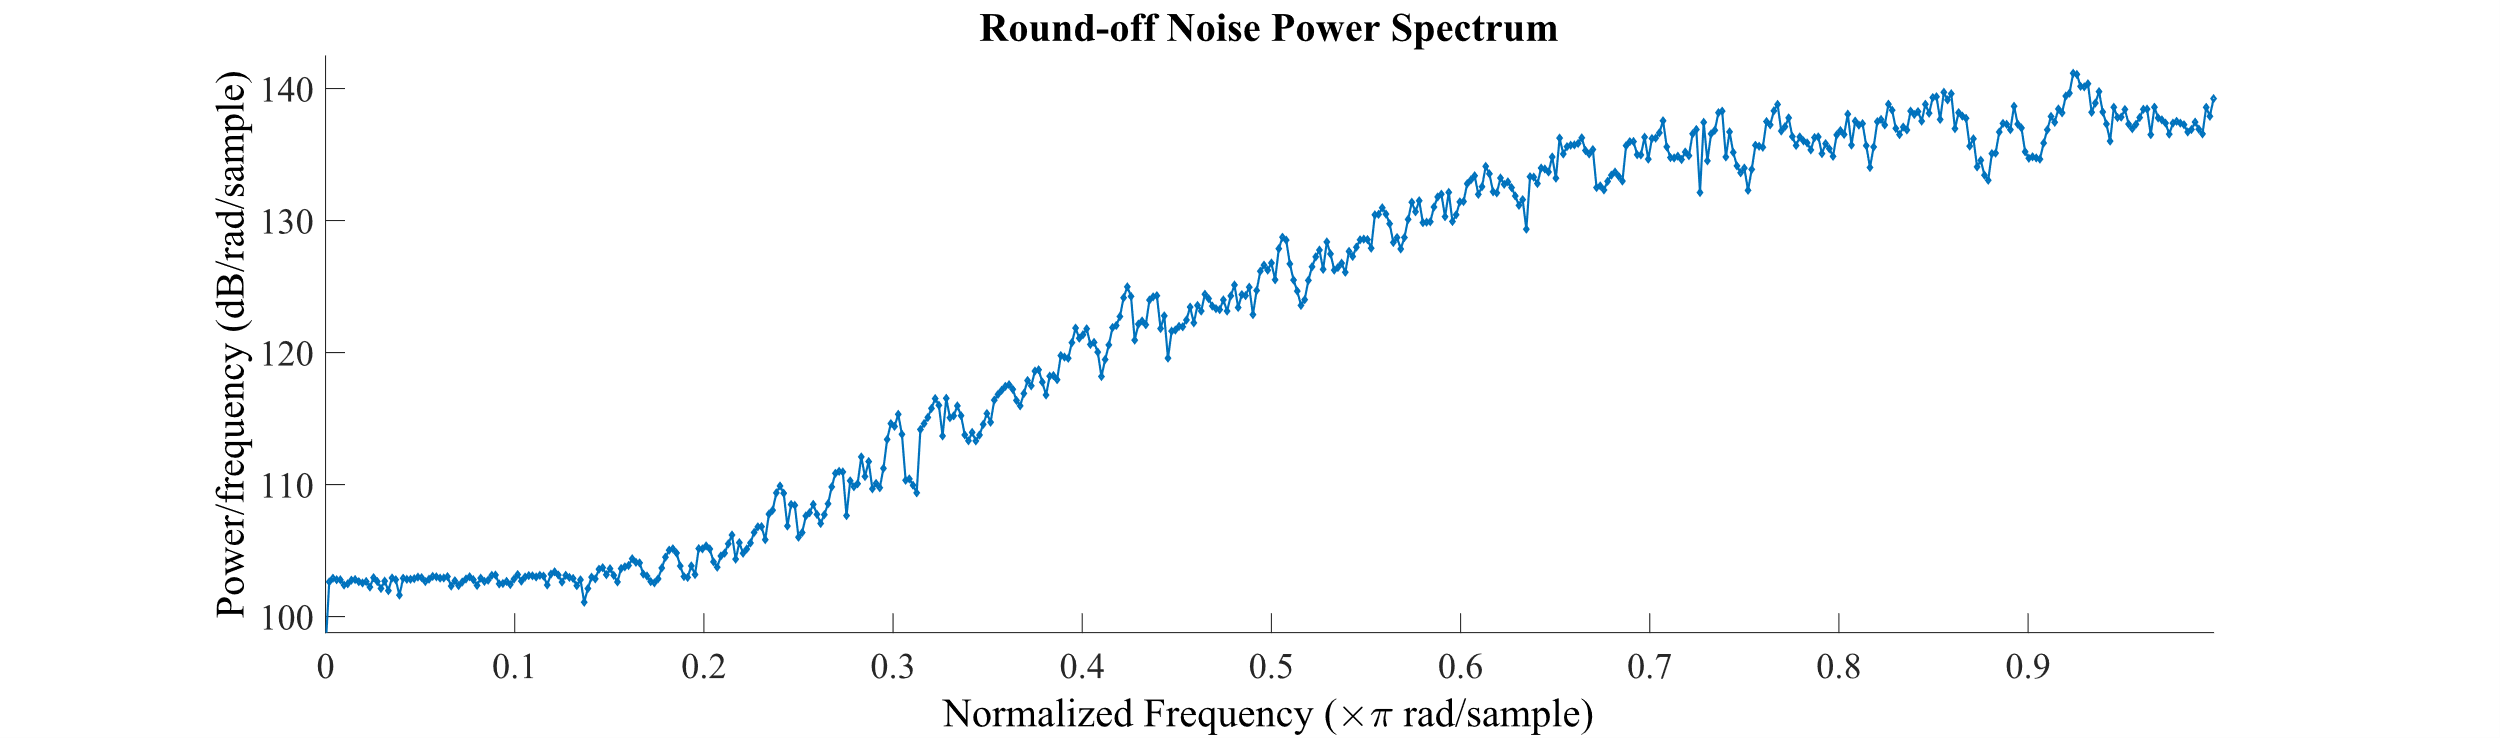
\includegraphics[width=6.46in,height=2.19in]{25}
		\caption{ Round-off noise Power Spectrum.}
		\label{fig:_11_Roundoff_noise_Power_Spectrum}
	\end{Center}
\end{figure}


%%%%%%%%%%%%%%%%%%%% Figure/Image No: 34 Ends here %%%%%%%%%%%%%%%%%%%%
The errors in a fixed-point finite impulse response (FIR) filter due to quantization (analog-to-digital conversion) and roundoff are considered. Expressions for the exact moments of the filter output noise are derived. It is well known that, when the input signal satisfies certain conditions, the popular additive white noise model can be valid in describing the quantization noise. The characteristics of multiplicative roundoff noises, however, differ from what this model predicts, even under conditions where the roundoff noises are white. Hence the additive white noise model does not provide accurate results on the characteristics of the output error in an FIR filter. Using the exact formulas for the moments, the author computes the exact power spectrum of the filter output error. These results agree well with those obtained from simulation.
\par

\par



\vspace{\baselineskip}


%%%%%%%%%%%%%%%%%%%% Figure/Image No: 35 starts here %%%%%%%%%%%%%%%%%%%%

\begin{figure}[H]
	\begin{Center}
		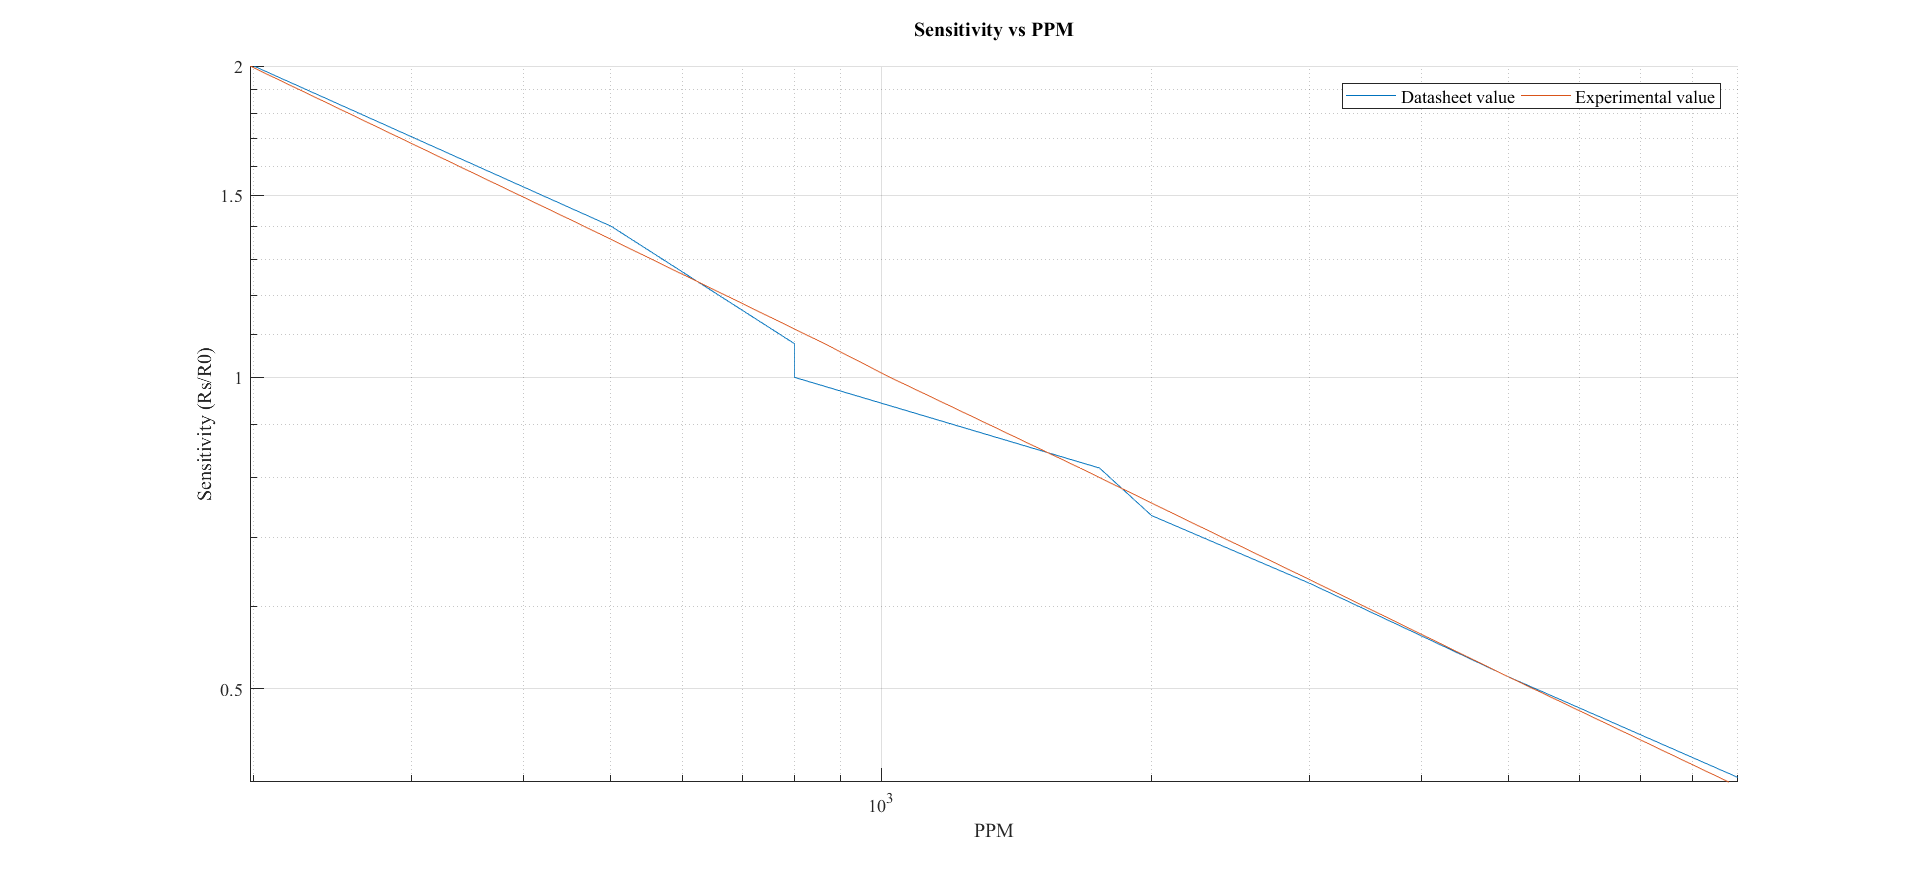
\includegraphics[width=6.42in,height=3.33in]{26}
		\caption{Sensitivity vs PPM graph. (Log-Log plot)}
		\label{fig:_12_Sensitivity_vs_PPM_graph_LogLog_plot}
	\end{Center}
\end{figure}


%%%%%%%%%%%%%%%%%%%% Figure/Image No: 35 Ends here %%%%%%%%%%%%%%%%%%%%

\par

\par
\begin{justify}
Figure 7.12 shows the actual $\&$  experimental Sensitivity vs Concentration plot, from where it can be said that the calibration was 90-95$\%$  accurate, which is good.
\end{justify}\par

\vspace{\baselineskip}


%%%%%%%%%%%%%%%%%%%% Figure/Image No: 36 starts here %%%%%%%%%%%%%%%%%%%%

\begin{figure}[H]
	\begin{Center}
		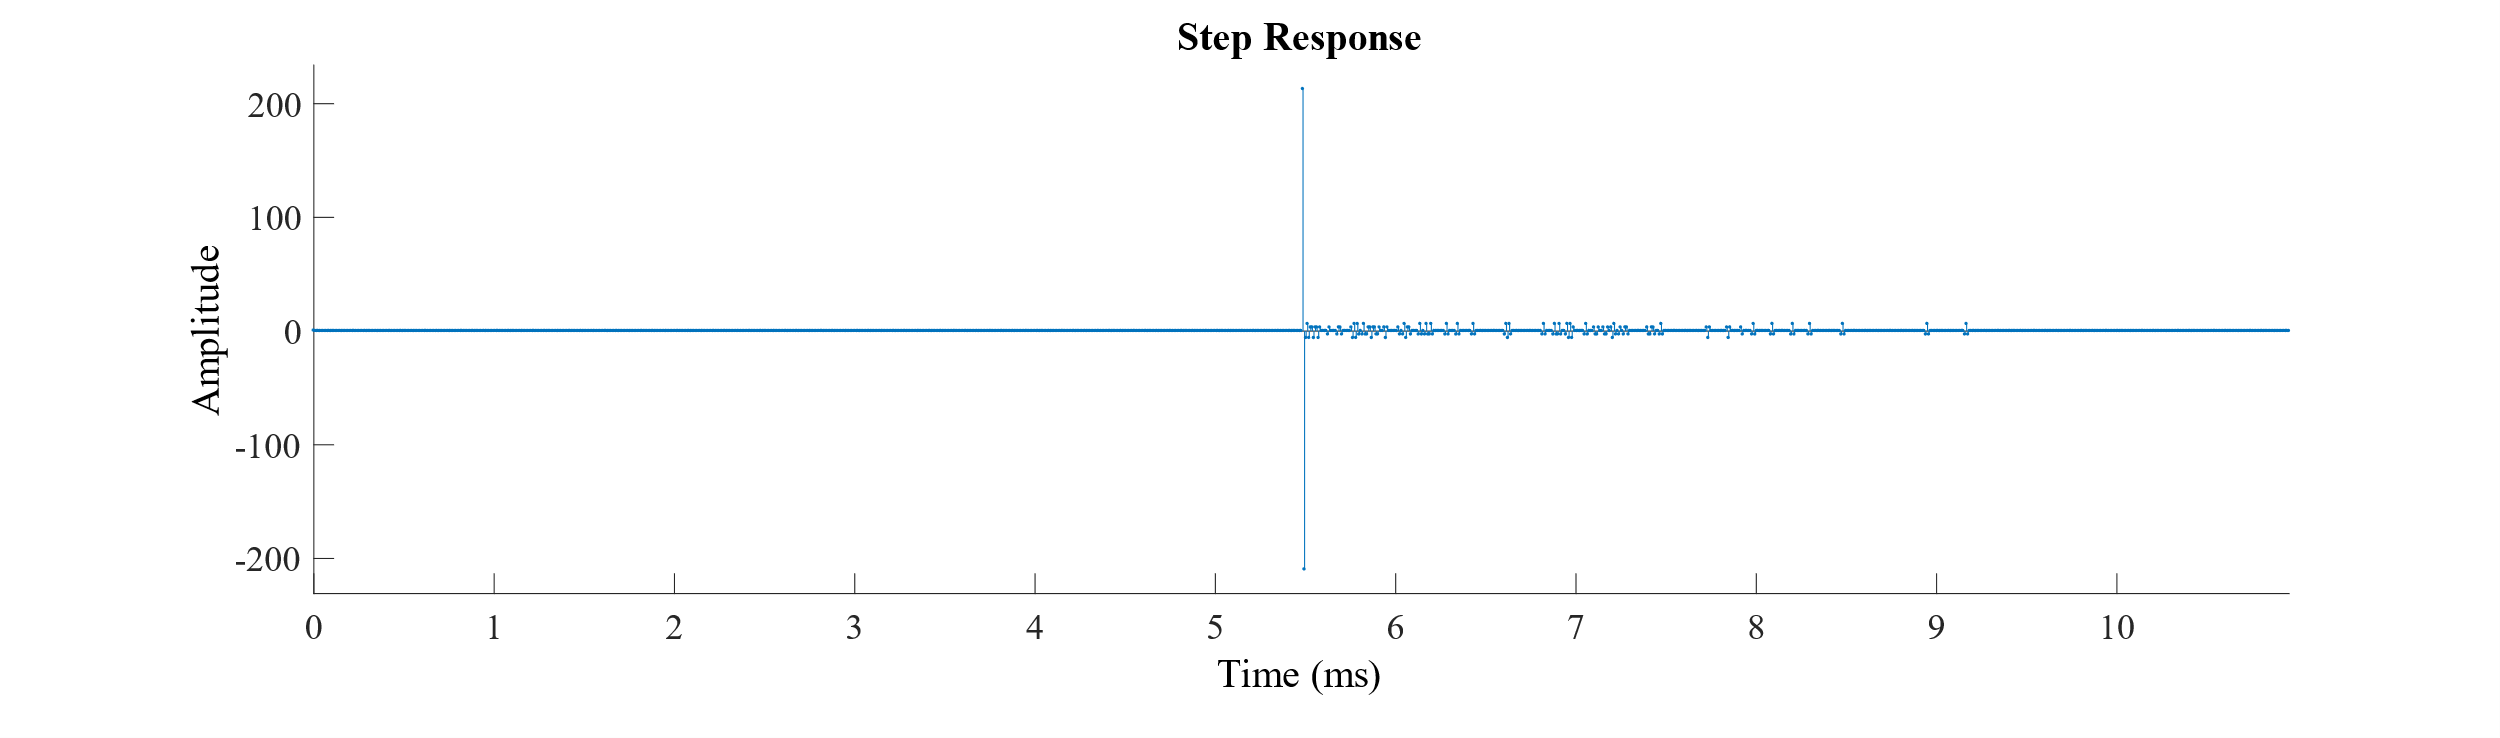
\includegraphics[width=6.5in,height=2.22in]{27}
	\end{Center}
\caption{Step response.}
\end{figure}


%%%%%%%%%%%%%%%%%%%% Figure/Image No: 36 Ends here %%%%%%%%%%%%%%%%%%%%

\par

\par

\begin{justify}
From, Figure 7.13, the step response can be shown where it is seen that initially the system runs fine but after a certain period it shows some abrasions but the used filter automatically fixes the errors. The below, Figure 7.14 shows the time domain and frequency domain analysis plot for the system.
\end{justify}\par



%%%%%%%%%%%%%%%%%%%% Figure/Image No: 37 starts here %%%%%%%%%%%%%%%%%%%%

\begin{figure}[H]
	\begin{Center}
		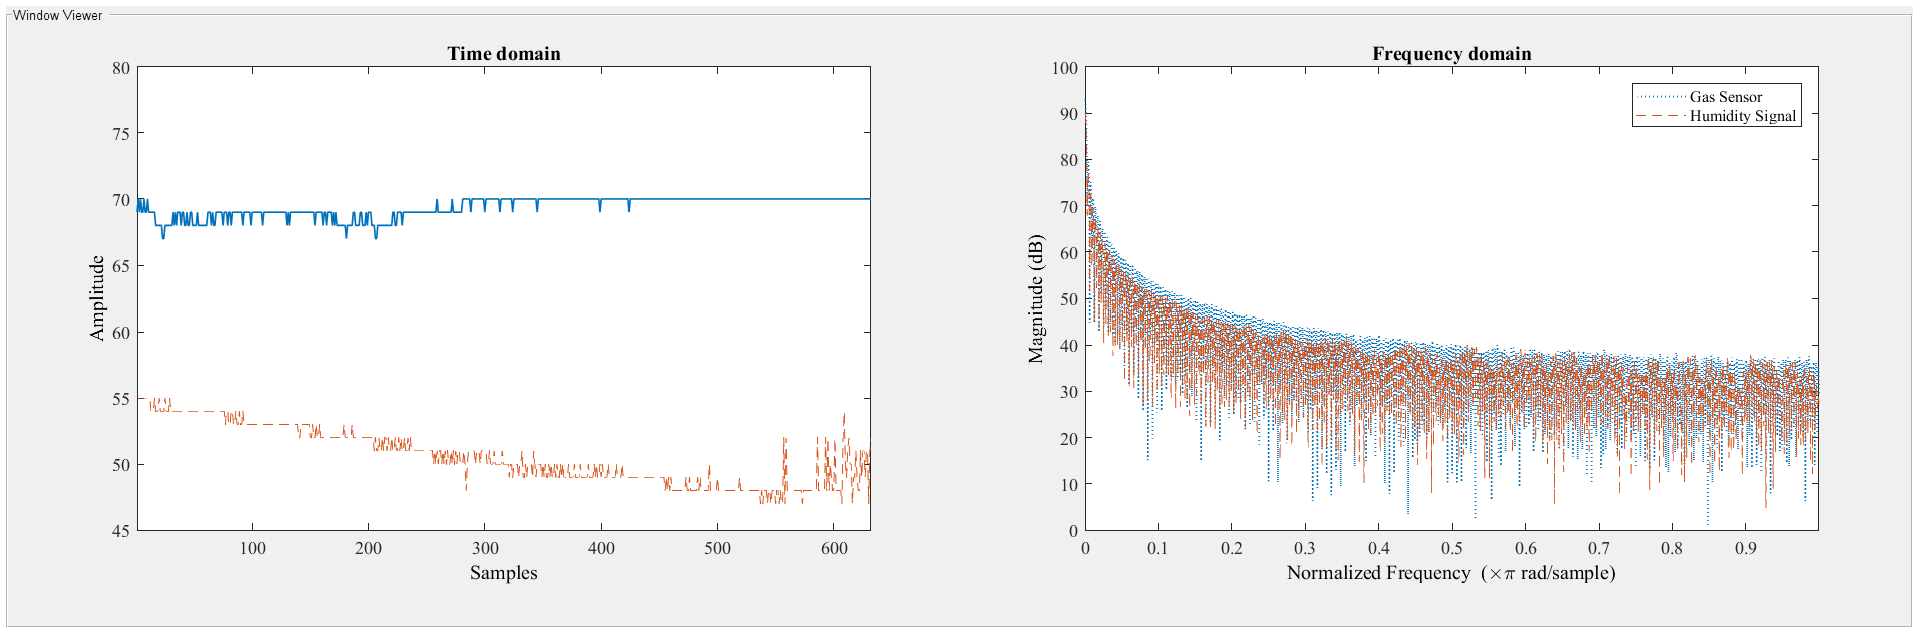
\includegraphics[width=6.53in,height=2.27in]{28}
		\caption{Time domain and Frequency domain graph for the system.}
		\label{fig:_14_Time_domain_and_Frequency_domain_graph_for_the_system}
	\end{Center}
\end{figure}


%%%%%%%%%%%%%%%%%%%% Figure/Image No: 37 Ends here %%%%%%%%%%%%%%%%%%%%

\par

\par

\begin{justify}
The transfer function of the system can be estimated by using Welch Transfer function distribution theory, which is plotted on Figure 7.15. The Figure 7.16 shows the experimental relation between supplied voltage and gas concentration.
\end{justify}\par



%%%%%%%%%%%%%%%%%%%% Figure/Image No: 38 starts here %%%%%%%%%%%%%%%%%%%%

\begin{figure}[H]
	\begin{Center}
		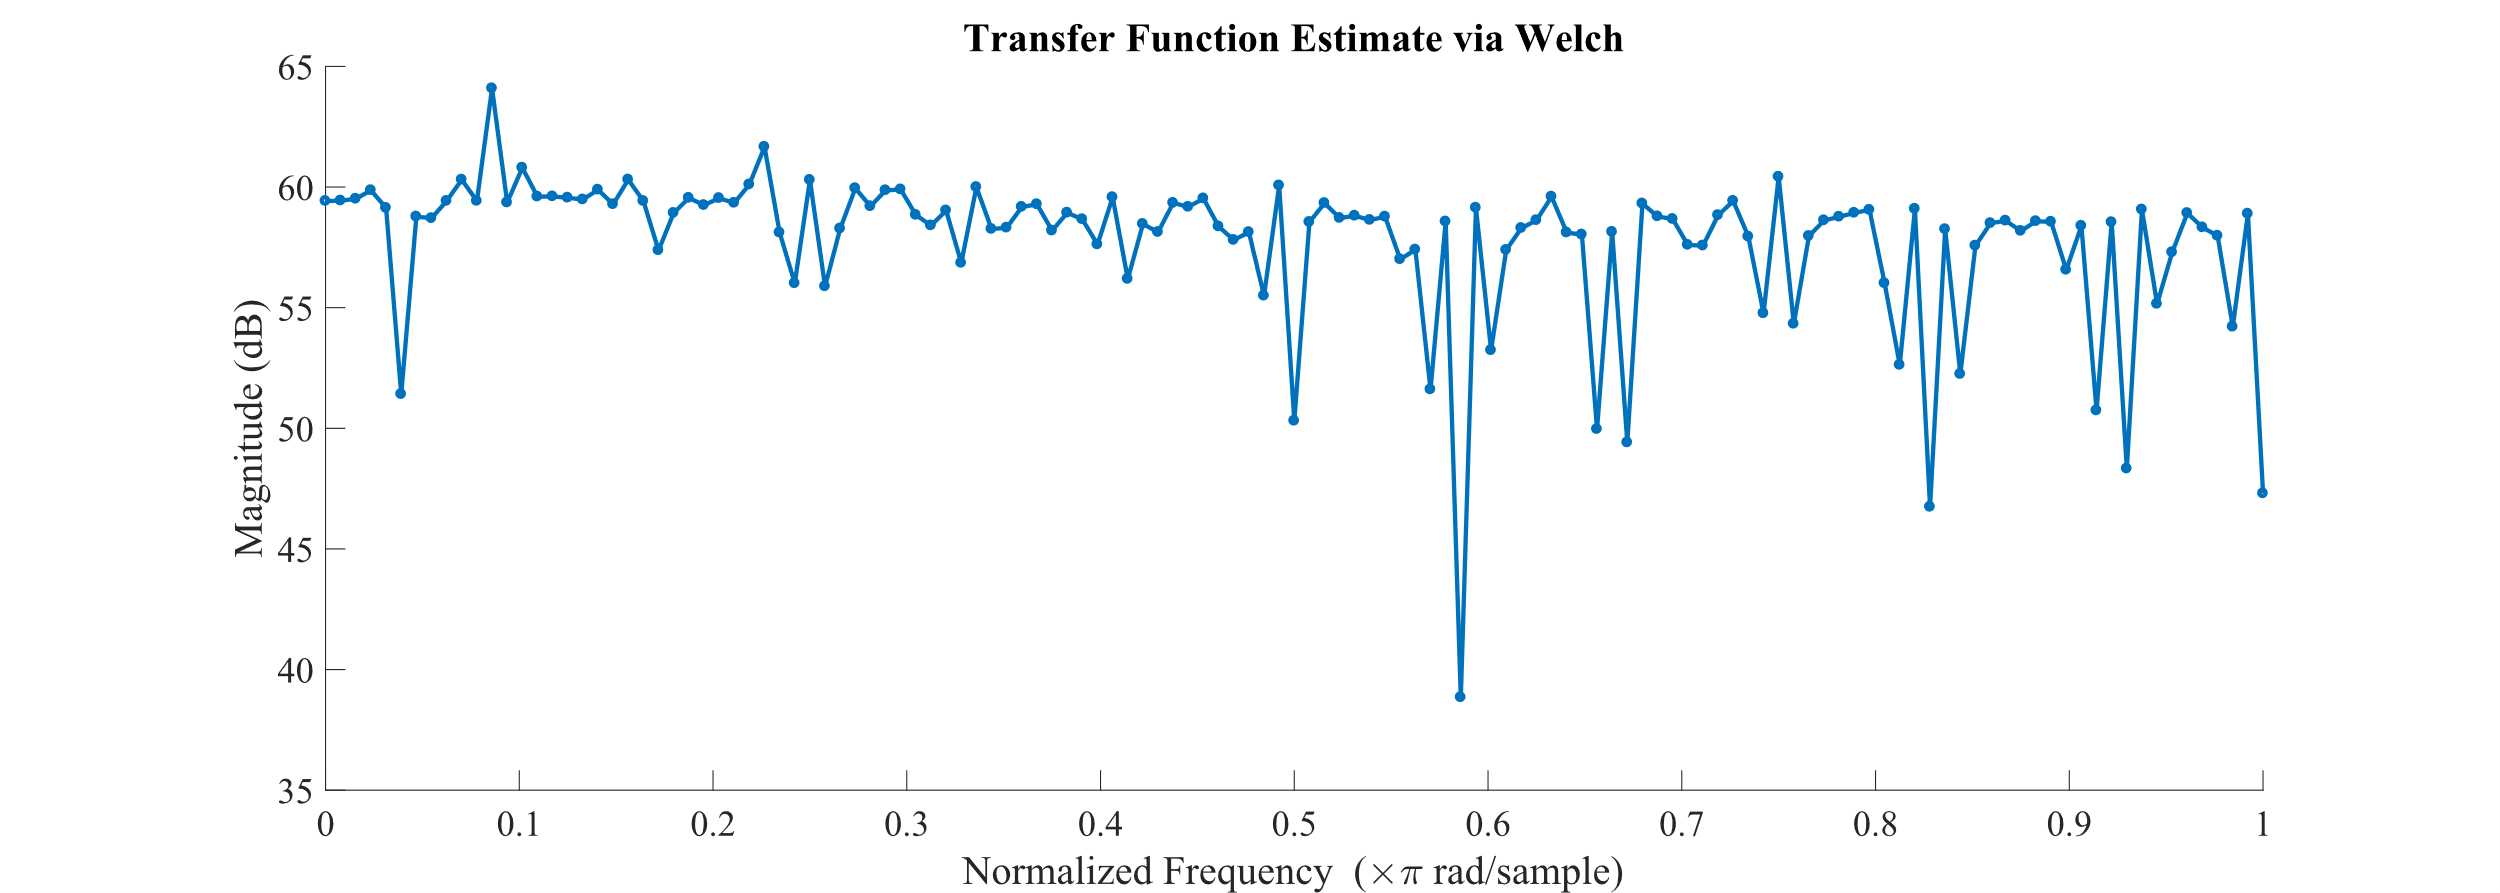
\includegraphics[width=6.51in,height=2.44in]{29}
		\caption{Transfer function estimation via Welch distribution.}
		\label{fig:_15_Transfer_function_estimation_via_Welch_distribution}
	\end{Center}
\end{figure}


%%%%%%%%%%%%%%%%%%%% Figure/Image No: 38 Ends here %%%%%%%%%%%%%%%%%%%%

\par

\par


\vspace{\baselineskip}


%%%%%%%%%%%%%%%%%%%% Figure/Image No: 39 starts here %%%%%%%%%%%%%%%%%%%%
%
%\begin{figure}[H]
%	\begin{Center}
%		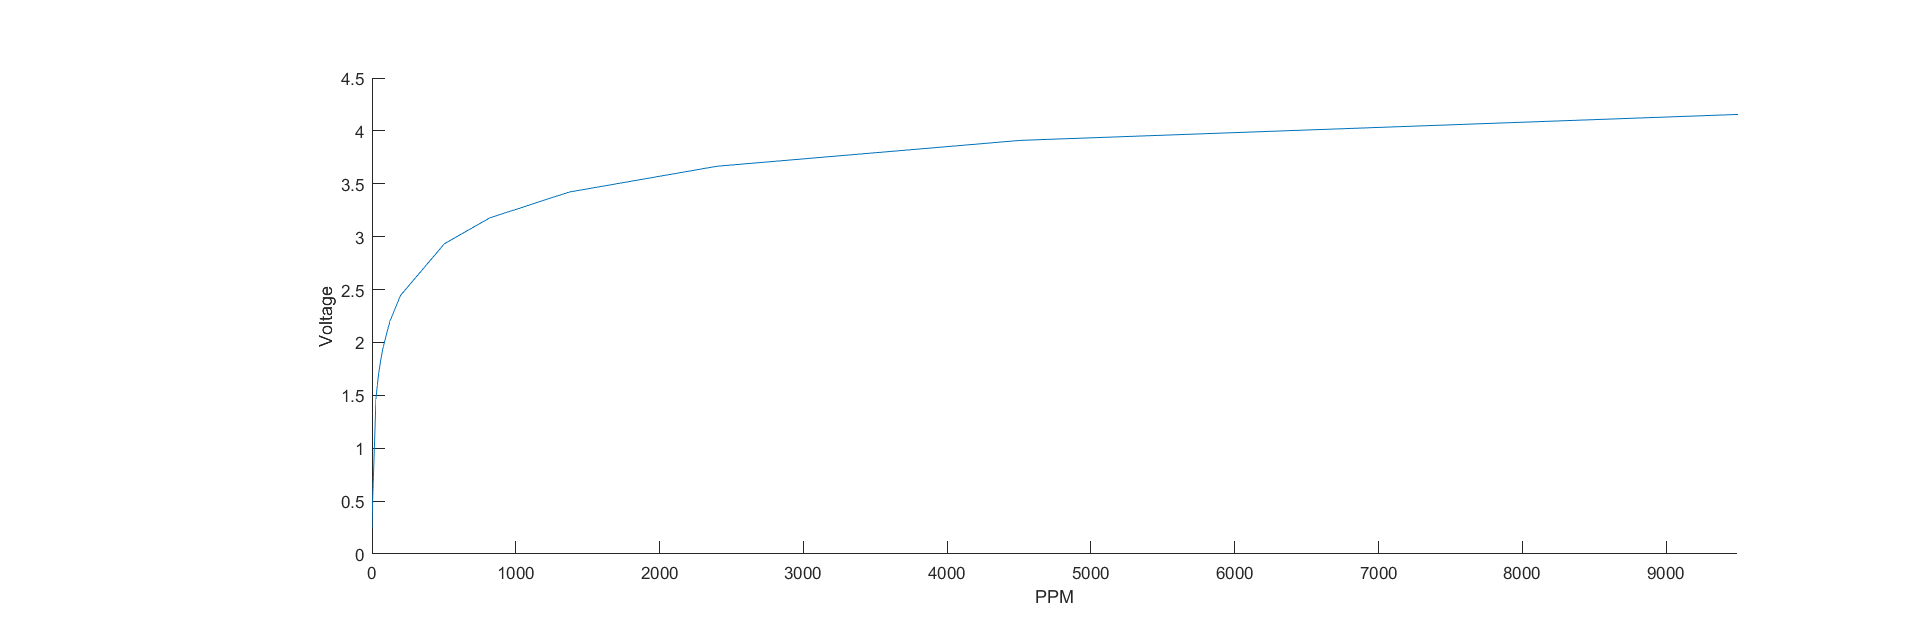
\includegraphics[width=6.37in,height=2.38in]{30}
%		\caption{Voltage vs PPM graph.}
%		\label{fig:_16_Voltage_vs_PPM_graph}
%	\end{Center}
%\end{figure}


%%%%%%%%%%%%%%%%%%%% Figure/Image No: 39 Ends here %%%%%%%%%%%%%%%%%%%%

\par

\par

\item \textbf{Power Spectrum Density Analysis (PSE or PSD):} PSE is most important application area in Digital Signal Processing. There are
mainly two types of power spectrum estimation (PSE) method: Parametric and nonparametric. Parametric or non-classical methods an analyzed process is place by an appropriate model with known spectrum. Non-parametric do not make any assumption on the data generating process. It is start by estimating autocorrelation sequence from a given data. The power spectrum then is estimated via FT of an estimated autocorrelation sequence. Window function is a mathematical function that is zero valued outside of some chosen period. When another unction or waveform or data sequence is multiplied by a window function, the product is also zero-valued outside the period; all that is left is the part where they overlap the observation through the window. It is simple to apply and understand. In this method the frequency of a filter, HD(w) and the corresponding impulse response, hD(n), are related by the inverse Fourier transform \cite{cheikhrouhou2018hybrid,khelifi2018localization,choosaksakunwiboon2018pre}:


\begin{equation}\tag{7.13}
h_{D} ( n ) = \frac{1}{2 \pi } \int _{- \pi }^{ \pi }H_{D} ( w ) e^{iwn}dw
\end{equation}
\begin{justify}
Where HD(w) is frequency response of a filter and hD(n) is corresponding impulse response. The subscript D is used to make a difference between the ideal and practical responses. Here, HD(w) can be obtained from hD(n) by evaluating the inverse Fourier transform. The truncation of hD(n) to a length M-1 is equivalent to multiplying hD(n)by a rectangular window [2] defined as:
\end{justify}\par


\begin{equation}\tag{7.14}
w ( n ) = \{ \begin{array}{ll}
	1,~ \&n=0,1,2, \ldots .. ( M-1 ) \\
	0,~ \&otherwise\\
	\end{array}
\end{equation}
\begin{justify}
And unit impulse response will be:
\end{justify}\par


\begin{equation}\tag{7.15}
h ( n ) =h_{D} ( n ) .w ( n )
\end{equation}

\begin{equation}\tag{7.16}
h ( n ) = \{ \begin{array}{ll}
	h_{D} ( n ) ,~ \&n=0,1,2, \ldots .. ( M-1 ) \\
	0,~ \&otherwise\\
	\end{array}
\end{equation}
\begin{justify}
Frequency domain function in representation of window function is,
\end{justify}\par


\begin{equation}\tag{7.17}
W ( w ) = \sum _{n=0}^{M-1}w ( n ) .e^{-jwn}
\end{equation}
\begin{justify}
The individuality of it play a significant role in establishment of the resulting frequency response of the finite impulse response filter obtained by truncation hD(n) to length M. The undesirable effects are best alleviated by the use of window that do not contain abrupt discontinuities in their time domain characteristics and have likewise low side lobes in their frequency domain characteristics. For the same value of M for both Rectangular and Hamming window or other windows, the width of the main lobe is also wider for these windows compared to the rectangular window. The Fourier transform of rectangular window \cite{movlaee2018microwave,goutham2018flexible,arif2018gait,tischler2018system,sloo2018smart,losey2018review,yilmaz2018pv,he2017adaptive,walczak2019artificial,comer2018internet}:
\end{justify}\par


\begin{equation}\tag{7.18}
W ( w ) = \sum _{n=0}^{M-1}e^{-jwn}
\end{equation}
\begin{justify}
On simplification equation-(7.18) reaches,
\end{justify}\par


\begin{equation}\tag{7.19}
W ( w ) = \sum _{n=0}^{M-1}e^{-jwn}=e^{-jw.\frac{ ( M-1 ) }{2}}.\frac{sin ( wM/2 ) }{sin ( w/2 ) }
\end{equation}
\begin{justify}
The Hamming window function in time domain decrease more gently towards zero on either side and in frequency domain, the amplitude of the main lobes is wider approximately double than that of rectangular window, but side lobes are lesser relative to the main lobe about 40 dB down the main lobes, compared with 14 dB for the rectangular window. Hamming window lead to a filter with wider transition width but higher stopband attenuation.
\end{justify}\par


\begin{equation}\tag{7.20}
Y ( n ) =x ( n ) .w ( n )
\end{equation}
\begin{justify}
Where Y(n) is output signal x(n) is input signal, and w(n) [1] is window function.
\end{justify}\par


\begin{equation}\tag{7.21}
w ( n ) =0.54+0.46cos ( \frac{2 \pi }{N} ) ,~ where \{ \begin{array}{ll}
	-\frac{N}{2} \leq n \leq \frac{N}{2}  ( N=Even number ) \\
	- ( N-2 )  \leq n \leq \frac{ ( N-1 ) }{2} ( N=odd number ) \\
	\end{array}
\end{equation}
\begin{justify}
Transition width,  \(  \Delta f=\frac{3.3}{N} \) . Where N is filter length, and $ \Delta $ \textit{f} is normalized transition width Window Length, L = N+1. In Power Spectrum Estimation is most important application area in Digital Signal Welch method have two basic modification to the normal analytic method. These are allowed the data length to overlap. The data segment can be represented as,
\end{justify}\par


\begin{equation}\tag{7.22}
x ( n ) =x ( n+iD )  \{ \begin{array}{ll}
	n=0,1,2, \ldots  \ldots . ( M-1 ) \\
	i=0,1,2, \ldots  \ldots  \ldots . ( L-1 ) \\
	\end{array}
\end{equation}
\begin{justify}
Where iD is the starting point for the ith sequence. If D = M, the segment does not overlap and the L of data sequence is identical to the data segment of Bartlett method. The second change in Welch method is to window the data segments prior to computing the periodogram \cite{liu2018survey}.
\end{justify}\par


\begin{equation}\tag{7.23}
P_{xx}^{i} ( f ) =\frac{1}{MU} \vert  \sum _{n=0}^{M-1}x ( n ) .w ( n ) .e^{-j.2 \pi fn} \vert , where i=1,2, \ldots  \ldots  \ldots .. ( L-1 )
\end{equation}
\begin{justify}
Where U is a normalization factor for the power.
\end{justify}\par


\begin{equation}\tag{7.24}
U=\frac{1}{M} \sum _{n=0}^{M-1}w^{2} ( n )
\end{equation}
\begin{justify}
The Welch power spectrum estimate is the average of modified periodogram \cite{cheikhrouhou2018hybrid}, is
\end{justify}\par


\begin{equation}\tag{7.25}
P_{xx}^{w}=\frac{1}{L} \sum _{i=0}^{L-1}P_{xx}^{i} ( f )
\end{equation}
\begin{justify}
Mean value of Welch estimate,
\end{justify}\par


\begin{equation}\tag{7.26}
E [ P_{xx}^{w} ( f )  ] =\frac{1}{L} \sum _{i=0}^{L-1}E.P_{xx}^{i} ( f )
\end{equation}
\begin{justify}
The resolution of estimated power estimation is determined by the spectral resolution of each segment which is of length L, it is window dependent. From equations-(7.25) to (7.26), Figure 7.16 $\&$  Figure 7.17 can be drawn \cite{chatterjee2018artificial}.
\end{justify}\par



%%%%%%%%%%%%%%%%%%%% Figure/Image No: 40 starts here %%%%%%%%%%%%%%%%%%%%

\begin{figure}[H]
	\begin{Center}
		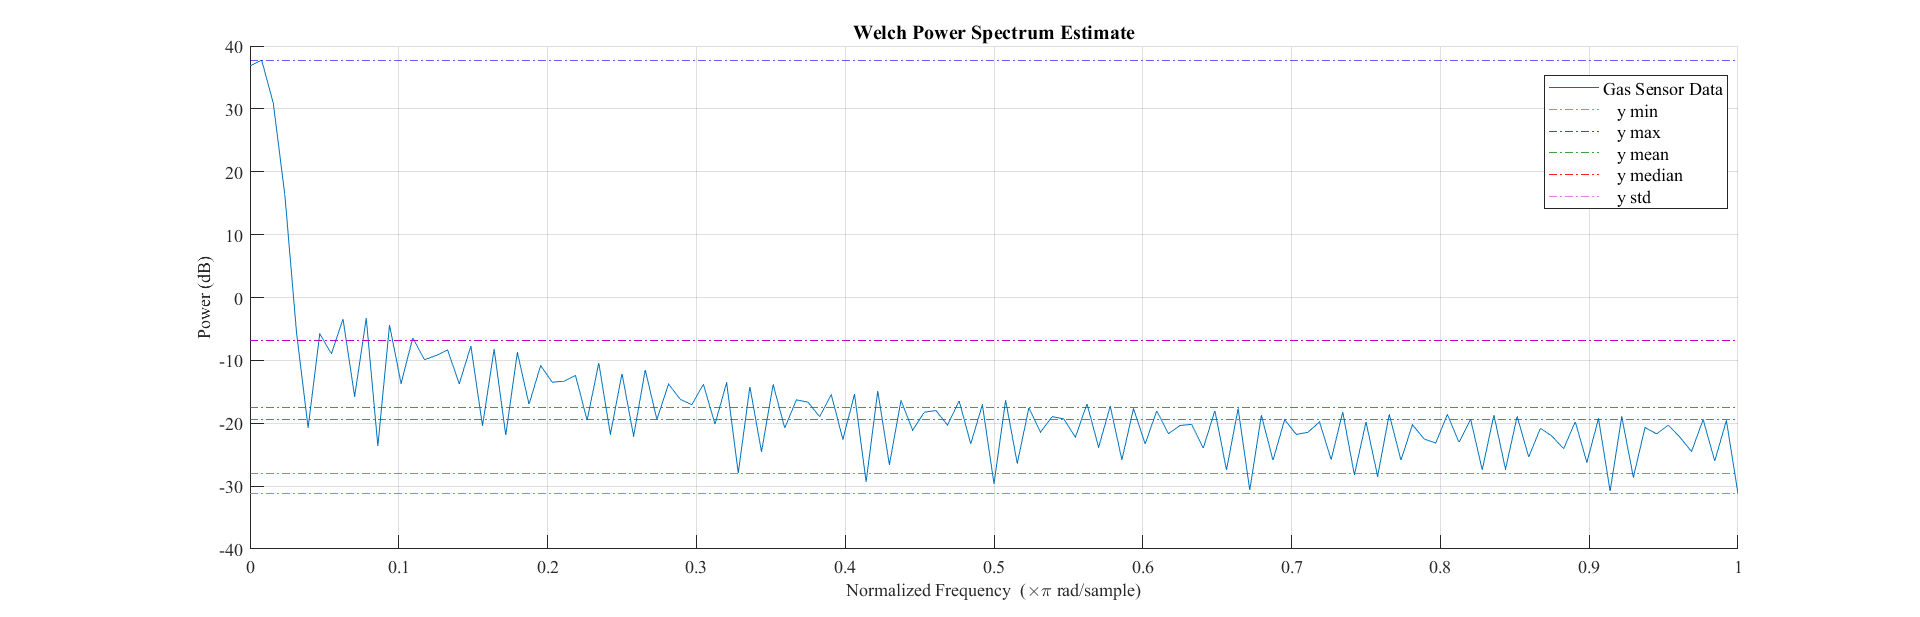
\includegraphics[width=6.61in,height=2.4in]{31}
		\caption{Welch power spectrum estimate for Gas sensor.}
		\label{fig:_17_Welch_power_spectrum_estimate_for_Gas_sensor}
	\end{Center}
\end{figure}


%%%%%%%%%%%%%%%%%%%% Figure/Image No: 40 Ends here %%%%%%%%%%%%%%%%%%%%

\par

\par


\vspace{\baselineskip}


%%%%%%%%%%%%%%%%%%%% Figure/Image No: 41 starts here %%%%%%%%%%%%%%%%%%%%

\begin{figure}[H]
	\begin{Center}
		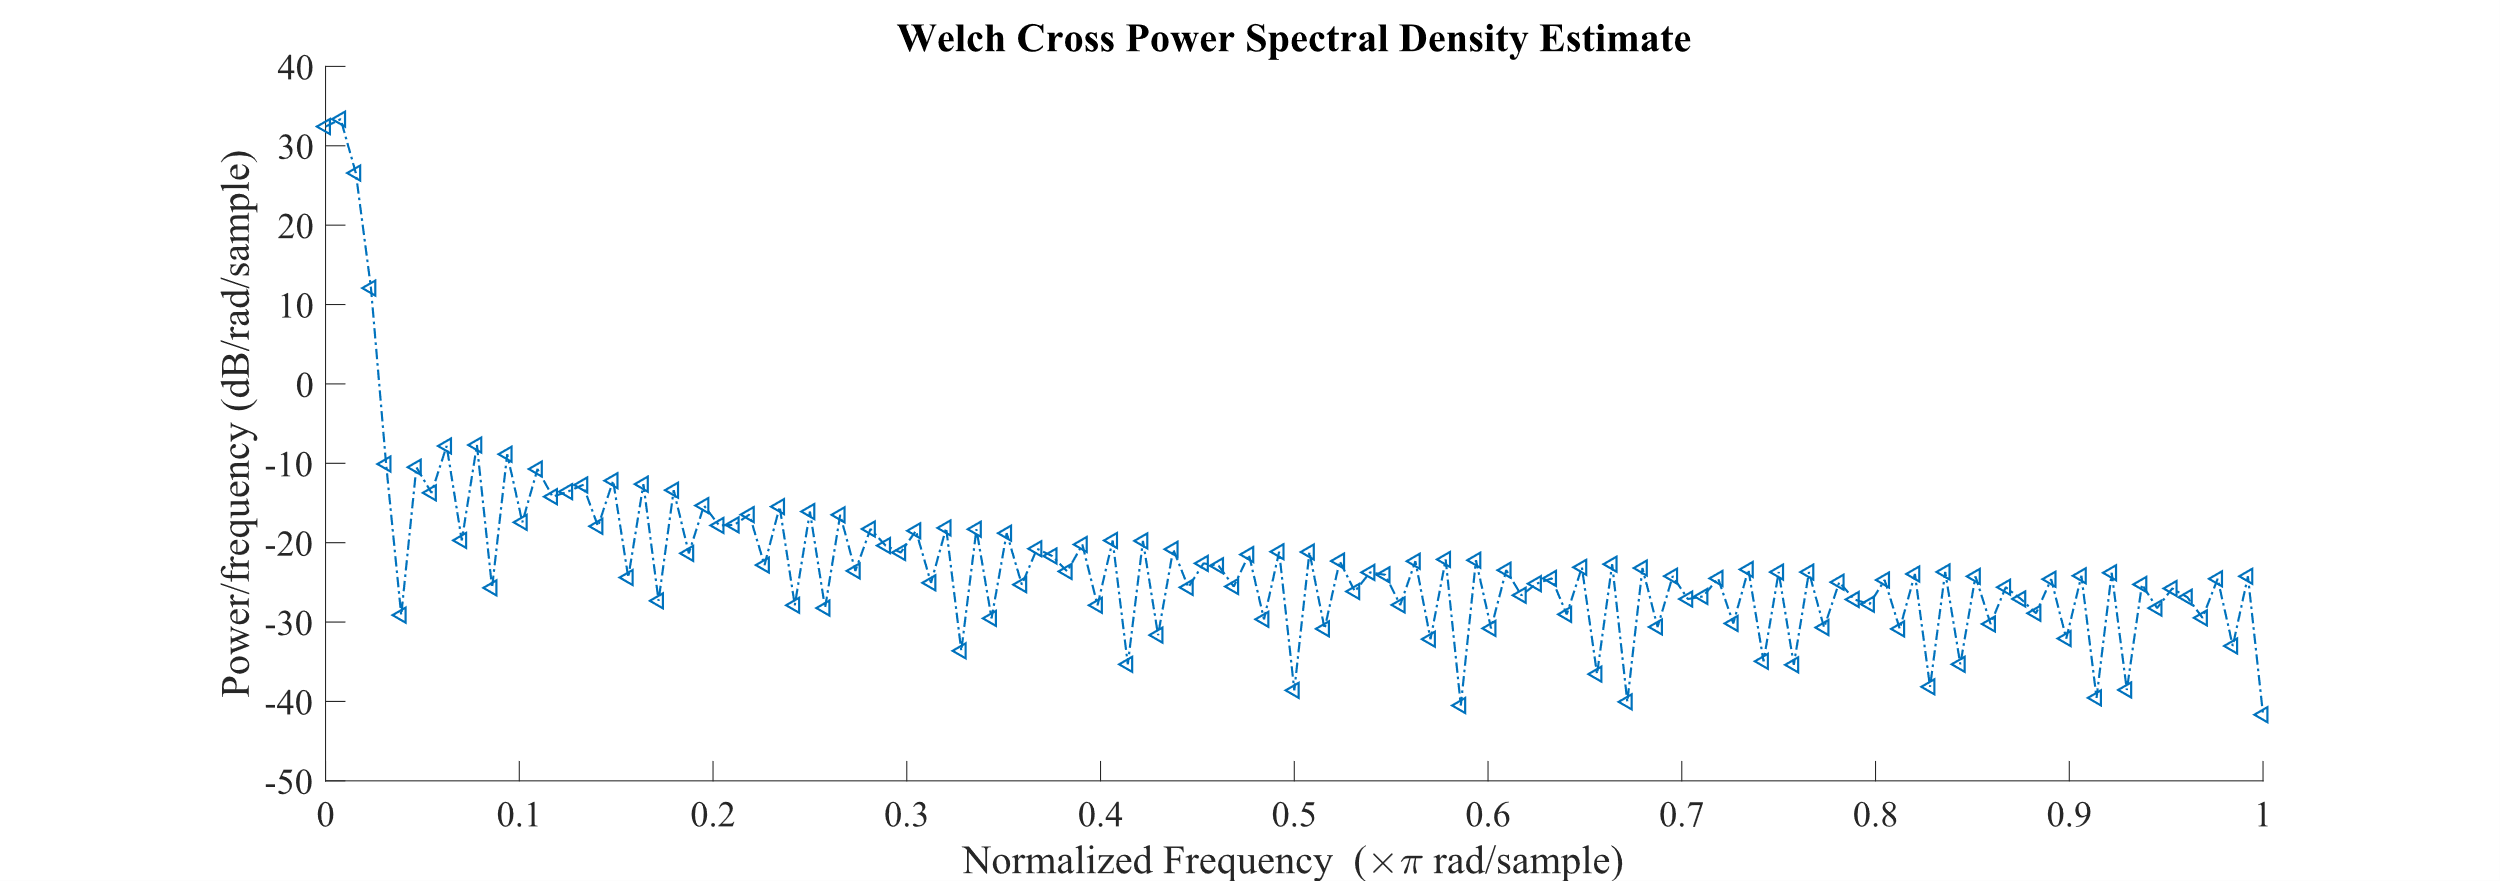
\includegraphics[width=6.52in,height=2.59in]{32}
	\end{Center}
\caption{Welch Cross power density estimate.}
\end{figure}


%%%%%%%%%%%%%%%%%%%% Figure/Image No: 41 Ends here %%%%%%%%%%%%%%%%%%%%

\par

\par
\end{enumerate}
\setlength{\parskip}{8.04pt}
\section{Feedback Control for the Controller }
\begin{justify}
In this system, the reference value is set at 2000 ppm of smoke concentrations. Whenever the controller gets a reading higher than 2000 ppm from the gas sensor then it automatically activates the actuators and the rise in concentration gets mitigated. Thus, the error in the system is eliminated very soon after it takes place in the plant. Fig. shows the schematic of the used feedback method of control for the proposed system.
\end{justify}\par



%%%%%%%%%%%%%%%%%%%% Figure/Image No: 42 starts here %%%%%%%%%%%%%%%%%%%%

\begin{figure}[H]
	\begin{Center}
		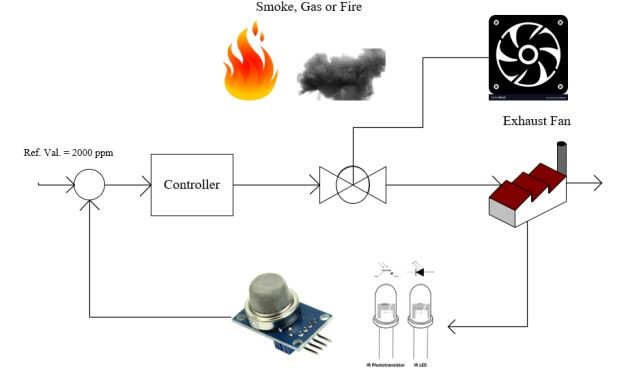
\includegraphics[width=4in,height=2in]{33}
		\caption{Schematic for feedback control system}
		\label{fig:_19_Schematic_for_feedback_control_system}
	\end{Center}
\end{figure}


%%%%%%%%%%%%%%%%%%%% Figure/Image No: 42 Ends here %%%%%%%%%%%%%%%%%%%%

\par

\par

\section{Feedforward Control for the Controller }
\begin{justify}
For the feedforward control, when any abruptions take place in any sensors, then it is very necessary to mitigate the error before it takes place in the plant. Thus, manual wireless switching is introduced here to control the abruptions. From the computer, the actuation signal buttons are pressed from the webpage which in regards sends a signal to the controller via\textit{ }a routing media (for this experiment a 300 mbps router is used). When the signal is received by the controller, a swift actuator switching takes place to mitigate the abruptions. Fig. shows the graphical representation of the proposed feedforward control system for the experimental setup.
\end{justify}\par



%%%%%%%%%%%%%%%%%%%% Figure/Image No: 43 starts here %%%%%%%%%%%%%%%%%%%%

\begin{figure}[H]
	\begin{Center}
		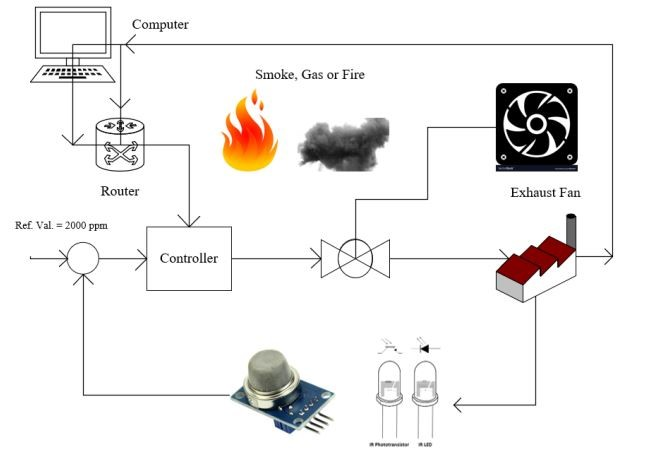
\includegraphics[width=4in,height=2in]{34}
		\caption{Schematic for feedforward control system}
		\label{fig:_20_Schematic_for_feedforward_control_system}
	\end{Center}
\end{figure}


%%%%%%%%%%%%%%%%%%%% Figure/Image No: 43 Ends here %%%%%%%%%%%%%%%%%%%%

\par

\par
\newpage

\vspace{\baselineskip}
\section{Data Security }
Data security refers to the process of protecting data from unauthorized access and data corruption throughout its lifecycle. Data security includes data encryption, tokenization, and key management practices that protect data across all applications and platforms.Cloud adoption is increasing risks of data breach, data loss, and non-compliance with data privacy regulations.
\subsection{Cryptographic nonce}
\begin{justify}
A nonce is a random or semi-random number that is generated for a specific use, typically related to cryptographic communication or information technology. The term itself stands for number used once  or number once  and is most commonly referred to specifically as a cryptographic nonce. Data was sent by adding an arbitrary value and when data was received by a controller it subtracted the arbitrary value by itself. The value was randomly selected by the user. If any attack will occur during data communication the attacker will get the data with the added arbitrary value.
\end{justify}\par
\section{Chapter Summery}
In this chapter all test result and data analysis was performed.Data analysis using different types of filtering method and algorithms was also performed in this chapter and data security of the system also explained here for the security purposes.Althouth system stability and performance of the system also be determined in this chapter. 
\chapter{\textbf{Conclusion}}
The fabricated system run successfully and 20 trials were performed to measure its performance. It showed no errors in those 20 trials which took almost 3 hours to execute. The control system took almost 1 seconds (approximately) to perform necessary commands when signals came from the host server. From analyzed signals the impulse period and the group delay period seemed quite perfect if the Baud Rate (Sampling Frequency) tuning ranges from 11 to 12.6 kHz. In this dissertation, 11.52 kHz Sampling Frequency was used and the power density spectrum of gas sensor was quite fine though the Signal to Noise ratio was a little high. This can be overcome by using a 20 pF ceramic disk capacitor as it can work as a low pass filter. The overall system efficiency was about 95$\%$ , which is quite good for a robust controlling operation.\\
Work With the continuous development in technology and availability of internet it is possible to develop a low-cost smart sensor node which enables things to be connected and monitored easily and corresponding information can be accessible globally. An integrated framework is
developed with the combination of WSN and Local IP. The promising issue of the proposed method is to provide a flexible low-cost solution for integrating Local IP  with home automation or Industrial automation systems. A real time application of WSN for the development of smart home or industry is designed and implemented. The smart environment is created by adapting different types of sensors and actuators which are used to communicate with things through webpage over the internet. The gathered sensor data from different sensor node are displayed in the user dashboard. User can monitor the environment and control the physical objects. Also, to give more intelligence to the home devices, a decision-making algorithm is designed based on http request.
\section{Future Research Directions}
This framework can be extended for the development of building and city automation and Industry 4.0. Also, the WSN based control scheme can be extended for controlling and monitoring of remote devices such as robots, different types of rovers etc. Though there are numerous future scopes of the project, some of this are listed below
The web page further can be developed to provide real time chart for better visualization of sensor node data in an android APK app for the Android users.\\
Voice commands technology can be implemented for controlling Actuators.\\
Adaptive fuzzy logic can be implemented for automatic controlling of AC, water pump and other equipment’s. It can also be used to pre-detect the probability of the fire.Fuzzy logic can be  implemented for the control of environment temperature. The decision-making system can provide 99:2\% accuracy with respect to the MATLAB simulation results.\\
The web page further can be developed to provide real time chart for better visualization of sensor node data. Power consumption of the equipment’s can also be presented in the webpage.\\
Image processing can be implemented to find out known and unknown faces. It can be used as security purposes by detecting faces.

%\include{appendix}



\bibliographystyle{IEEEtran}
\renewcommand{\bibname}{\textbf{References}}
\bibliography{acc}
\bibliographystyle{unsrt}%{adfathesis}%{IEEEtran}
\end{document} 